The following section seeks to outline the governing equations used within \emph{PowerCycle}, which was inspired by Lorenzo Galieti's codebase \emph{wopycle} \cite{Galieti2023}. 

\section{Architecture}
    At its core \emph{PowerCycle} is comprised of a fluid properties calculation engine and power plant equipment models, see Section~\ref{sec:prosim_fluid_props} and \ref{sec:prosim_components}, which form the building blocks of the power plant. The thermodynamic and techno-economic performance of the power plant can then be calculated for a given set of boundary conditions, and process parameters can be optimised to maximise the thermodynamic or techno-economic performance, see Figure~\ref{fig:powercycle}.

    \begin{figure}[H]
        \centering
        \resizebox{16cm}{!}{
            \begin{tikzpicture} [node distance=1.4cm]

    \definecolor{level1}{RGB}{218,227,243}
    \definecolor{level2}{RGB}{180,199,231}
    \definecolor{level3}{RGB}{143,170,227}
    \definecolor{level4}{RGB}{115,149,211}
    \definecolor{orchid227119194}{RGB}{227,119,194}
    \definecolor{sienna1408675}{RGB}{140,86,75}
    
    \node (BCs_bkg) [process, minimum height=5.8cm, text width=2.7cm, minimum width=2cm, fill=level2] {};
    \node (Ts)  [process, yshift=0.7cm, minimum height= 1.2cm, text width=2.3cm, minimum width=2cm, fill=level1] {Temperature};
    \node (BCs)  [process, above of=Ts, minimum height= 1.2cm, text width=2.3cm, minimum width=2cm, draw=none, fill=none] {\textbf{Boundary Conditions}};
    \node (Qs)  [process, yshift=-0.7cm, minimum height= 1.2cm, text width=2.3cm, , minimum width=2cm, fill=level1] {Vapour Quality};
    \node (Cs)  [process, below of=Qs, minimum height= 1.2cm, text width=2.3cm, minimum width=2cm, fill=level1] {CO\textsubscript{2} Content};


    \node (Opt_bkg) [process, right of=BCs_bkg, xshift=10.2cm, yshift=0.1cm, minimum height=14.2cm, minimum width=2cm, text width = 19.3cm, fill=level4] {};
    \node (Opt) [process, at=(Opt_bkg), yshift=6.1cm, minimum height=1.2cm, minimum width=2cm, text width = 3cm, draw=none, fill=none] {\textbf{Optimisation}};
    
    
    \node (Ctrls_bkg) [process, right of=BCs_bkg, xshift=2.1cm, minimum height=10cm, minimum width=2cm, text width=2.7cm, fill=level2] {};
    \node (Pmax)  [process, at=(Ctrls_bkg), minimum height= 1.2cm, text width=2.3cm, minimum width=2cm, fill=level1] {\(P_{max}\)};
    \node (Tcond)  [process, above of=Pmax, minimum height= 1.2cm, text width=2.3cm, minimum width=2cm, fill=level1] {\(T_{cond}\)};
    \node (Xflash)  [process, above of=Tcond, minimum height= 1.2cm, text width=2.3cm, minimum width=2cm, fill=level1] {\(X_{flash}\)};
    \node (Ctrls)  [process, above of=Xflash, minimum height= 1.2cm, text width=2.3cm, minimum width=2cm,  draw=none, fill=none] {\textbf{Controls}};
    \node (Tmax)  [process, below of=Pmax, minimum height= 1.2cm, text width=2.3cm, minimum width=2cm, fill=level1] {\(T_{max}\)};
    \node (Tmin)  [process, below of=Tmax, minimum height= 1.2cm, text width=2.3cm, minimum width=2cm, fill=level1] {\(T_{min}\)};
    \node (Ctrls_plus)  [process, below of=Tmin, minimum height= 1.2cm, text width=2.3cm, minimum width=2cm, fill=level1] {...};

    \node (PP_bkg) [process, right of=Ctrls_bkg, yshift=-0.2cm, xshift=6.6cm, minimum height=11cm, minimum width=2cm, text width = 12.1cm, fill=level3] {};
    \node (PP) [process, at=(PP_bkg), yshift=4.65cm, minimum height=1.2cm, minimum width=2cm, text width = 3cm, draw=none, fill=none] {\textbf{Power Plant}};

    \node (Fluids_bkg) [process, right of=Ctrls_bkg, xshift=2.1cm, minimum height=5.8cm, minimum width=2cm, text width=2.7cm,fill=level2] {};
    \node (Org)  [process, at=(Fluids_bkg), yshift=0.7cm, minimum height= 1.2cm, text width=2.3cm, minimum width=2cm, fill=level1] {Organic};
    \node (Fluids)  [process, above of=Org, minimum height= 1.2cm, text width=2.3cm, minimum width=2cm,  draw=none, fill=none] {\textbf{Fluids}};
    \node (Geo)  [process, at=(Fluids_bkg), yshift=-0.7cm, minimum height= 1.2cm, text width=2.3cm, minimum width=2cm, fill=level1] {Geofluid};
    \node (NCG)  [process, below of=Geo, minimum height= 1.2cm, text width=2.3cm, minimum width=2cm, fill=level1] {NCG};

    \node (Props)  [process, below of=NCG, yshift=-0.4cm, minimum height= 1.2cm, text width=2.3cm, minimum width=2cm, fill=level1] {Properties};


    \node (Comps_bkg) [process, right of=Fluids_bkg, xshift=3.45cm, minimum height=7.2cm, minimum width=2cm, text width=5.4cm, fill=level2] {};
    \node (HX)  [process, at=(Comps_bkg), xshift=-1.35cm, minimum height= 1.2cm, text width=2.1cm, minimum width=2.5cm, fill=level1] {Heat Exchanger};
    \node (Turb)  [process, above of=HX, minimum height= 1.2cm, text width=2.3cm, minimum width=2cm, fill=level1] {Turbine};
    \node (Comps)  [process, above of=Turb, xshift=1.3cm, minimum height= 1.2cm, text width=2.3cm, minimum width=2cm,  draw=none, fill=none] {\textbf{Components}};
    \node (Pump)  [process, below of=HX, minimum height= 1.2cm, text width=2.3cm, minimum width=2cm, fill=level1] {Pump};
    \node (Compr)  [process, below of=Pump, minimum height= 1.2cm, text width=2.3cm, minimum width=2cm, fill=level1] {Compressor};
    \node (Mix)  [process, right of=HX, xshift=1.3cm, minimum height= 1.2cm, text width=2.3cm, minimum width=2cm, fill=level1] {Mixer};
    \node (Sep)  [process, above of=Mix, minimum height= 1.2cm, text width=2.3cm, minimum width=2cm, fill=level1] {Separator};
    width=2cm] {Mixer};
    \node (Split)  [process, below of=Mix, minimum height= 1.2cm, text width=2.3cm, minimum width=2cm, fill=level1] {Splitter};
    \node (Comps_plus)  [process, below of=Split, minimum height= 1.2cm, text width=2.3cm, minimum width=2cm, fill=level1] {...};

    \node (Perf1)  [process, below of=Compr, yshift=-0.4cm, minimum height= 1.2cm, text width=2.3cm, minimum width=2cm, fill=level1] {Performance};
    \node (Cost1)  [process, below of=Comps_plus, yshift=-0.4cm, minimum height= 1.2cm, text width=2.3cm, minimum width=2cm, fill=level1] {Cost};


    \node (Solver)  [process, right of=Comps_plus, xshift=1.55cm, minimum height= 1.2cm, text width=2.3cm, minimum width=2cm, fill=level1] {\textbf{Cycle Solver}};
    \node (Cost2)  [process, above of=Solver, yshift=2.8cm, minimum height= 1.2cm, text width=2.3cm, minimum width=2cm, fill=level1] {Cost};
    \draw [arrow, ultra thick] ($(Solver) + (-0.5, 0.6)$) -- ($(Cost2) + (-0.5, -0.6)$);
    \node (Perf2)  [process, below of=Cost2, yshift=-0.2cm, minimum height= 1.2cm, text width=2.3cm, minimum width=2cm, fill=level1] {Performance};
    \draw [arrow, ultra thick] ($(Solver) + (0.5, 0.6)$) -- ($(Perf2) + (0.5, -0.6)$);


    \node (ObjFunc_bkg) [process, at=(Cost2), xshift=3.5cm, minimum height=5.8cm, minimum width=2cm, text width=2.7cm, fill=level2] {};
    \node (Perf3)  [process, at=(ObjFunc_bkg), yshift=0.7cm, minimum height= 1.2cm, text width=2.3cm, minimum width=2cm, fill=level1] {Performance};
    \node (ObjFunc)  [process, above of=Perf3, minimum height= 1.2cm, text width=2.3cm, minimum width=2cm,  draw=none, fill=none] {\textbf{Objective Function}};
    \node (Cost3)  [process, below of=Perf3, minimum height= 1.2cm, text width=2.3cm, minimum width=2cm, fill=level1] {Cost};
    \node (ObjFUnc_plus)  [process, below of=Cost3, minimum height= 1.2cm, text width=2.3cm, minimum width=2cm, fill=level1] {...};


    \node (Cons_bkg) [process, right of=Solver, xshift=2.1cm, yshift=-1.8cm, minimum height=4.4cm, minimum width=2cm, text width=2.7cm, fill=level2] {};
    \node (Pinch)  [process, at=(Cons_bkg), minimum height= 1.2cm, text width=2.3cm, minimum width=2cm, fill=level1] {\(\Delta T_{min}^{HX}\)};
    \node (Cons)  [process, above of =Pinch, minimum height= 1.2cm, text width=2.3cm, minimum width=2cm,  draw=none, fill=none] {\textbf{Constraints}};
    \node (Cons_plus)  [process, below of=Pinch, minimum height= 1.2cm, text width=2.3cm, minimum width=2cm, fill=level1] {...};

    \draw [arrow, ultra thick] (BCs_bkg) -- (Opt_bkg);
    \draw [arrow, ultra thick] (Ctrls_bkg) -- (PP_bkg);
    \draw [arrow, ultra thick] (Fluids_bkg) -- (Props);
    \draw [arrow, ultra thick] (Props) -| ++ (1.7, 1.55) |- (Comps_bkg);
    \draw [arrow, ultra thick] (Comps_bkg) -- (Perf1);
    \draw [arrow, ultra thick] (Comps_bkg) -- (Cost1);
    \draw [arrow, ultra thick] (Cost1) -| ($(Solver) + (-0.5, -0.6)$);
    \draw [arrow, ultra thick] (Perf1) |- ($(Cost1) + (0, -0.8)$) -| ($(Solver) + (0.5, -0.6)$);
    \draw [arrow, ultra thick] (PP_bkg) -- (ObjFunc_bkg);
    \draw [arrow, ultra thick] (PP_bkg) -- (Cons_bkg);

\end{tikzpicture}    
        }
        \caption{Component diagram of PowerCycle}
        \label{fig:powercycle}
    \end{figure}

\section{Fluid Properties}
    \label{sec:prosim_fluid_props}
    Underlying to all power plant component calculations are the thermophysical properties of the fluid(s) a given component is handling. However, as previously discussed in \nameref{ch:thermophysmodelling}, different fluids require different modelling approaches. 
    
    For example, pure fluids like idealised geofluids (i.e. water) or binary ORC working fluids (i.e. hydrocarbons and refrigerants) are best modelled with dedicated EOS, such as the \ac{WP} \ac{HEOS} for pure water. Such fluids can be modelled using calculation frameworks like \emph{CoolProp}, \emph{REFPROP}, \emph{FluidProp}, etc.  On the other hand, geofluids, which are complex mixtures of water, minerals and \ac{NCG}, require more flexible modelling approaches, such as \emph{GeoProp}.
    
    % or mixture specific models like the semi-empirical model for binary mixtures of water and carbon dioxide presented in Section \ref{sec:semiempirical_models}.

    From a modelling perspective, this poses a logistical problem because each calculation engine follows a unique syntax and workflow for obtaining and reporting thermophysical properties, and it is impractical to generate calculation engine specific component models. An alternative approach is the use of an unified fluid property modelling interface for the component models to interact with.

    The following section aims to provide details of the implementation of such a unified fluid property modelling interface and an overview of the calculation engines used in this work.

    \subsection{Architecture}
        The unified fluid property modelling interface is comprised of three key components: 1) the calculation engines, 2) the engine interfaces and 3) the front-end, which is accessible to the user.

        \begin{figure}[H]
            \centering
            \begin{tikzpicture} [node distance=1.5cm]

    \definecolor{blue_level1}{RGB}{218,227,243}
    \definecolor{blue_level2}{RGB}{143,170,227}
    \definecolor{green_level2}{RGB}{169,209,142}
    \definecolor{green_level1}{RGB}{226,240,217}
    \definecolor{gold_level1}{RGB}{255,242,205}
    \definecolor{gold_level2}{RGB}{255,217,102}
    \definecolor{red_level1}{RGB}{251,229,214}
    \definecolor{red_level2}{RGB}{244,177,131}

    \node (CP) [process, text width=1.8cm, minimum width=2cm, minimum height=1.2cm, fill=blue_level2] {CoolProp};
    \node (CP_inter) [process, right of=CP, xshift=2cm, text width=1.8cm, minimum width=2cm, minimum height=1.2cm, , fill=blue_level1] {Interface};

    \node (GP) [process, below of=CP, text width=1.8cm, minimum width=2cm, minimum height=1.2cm, fill=red_level2] {GeoProp};
    \node (GP_inter) [process, right of=GP, xshift=2cm, text width=1.8cm, minimum width=2cm, minimum height=1.2cm, fill=red_level1] {Interface};

    \node (other) [process, below of=GP, text width=1.8cm, minimum width=2cm, minimum height=1.2cm, fill=gold_level2] {...};
    \node (other_inter) [process, right of=other, xshift=2cm, text width=1.8cm, minimum width=2cm, minimum height=1.2cm, fill=gold_level1] {Interface};

    \node (fluid) [process, right of=GP_inter, yshift=0.2cm, xshift=3.7cm, text width=1.8cm, minimum width=4.5cm, minimum height=5.5cm, fill=green_level2] {};
    \node (fluid_label) [process, at=(fluid), xshift=-0.6cm, yshift=2.35cm, text width=1.8cm, draw=none, fill=none] {Fluid};
    \node (state) [process, right of=GP_inter, xshift=1.8cm, text width=1.4cm, minimum width=1.6cm, minimum height=4.2cm, fill=green_level1] {State};
    
    \node (update) [process, right of=state, xshift=1.8cm, text width=2.4cm, minimum width=2cm, minimum height=1.2cm, fill=green_level1] {Update( State Var1, State Var2)};
    \node (comp) [process, above of=update,yshift=0.2cm, text width=2.4cm, minimum width=2.2cm, minimum height=1.2cm, fill=green_level1] {Composition, Engine};
    \node (props) [process, below of=update,yshift=-0.2cm, text width=2.4cm, minimum width=2.2cm, minimum height=1.2cm, fill=green_level1] {Properties};

    \node [above of=CP, yshift=-0.5cm] {Engines};
    \node [above of=CP_inter, yshift=-0.5cm] {Interfaces};


    \draw [arrow, thick] (CP) to [out=10, in=170] (CP_inter);
    \draw [arrow, thick] (CP_inter) to [out=190, in=-10] (CP);
    \draw [arrow, thick] (CP_inter) to [out=10, in=170] ($(CP_inter)+(2.5,0.2)$);
    \draw [arrow, thick] ($(CP_inter)+(2.5,-0.2)$) to [out=190, in=-10] (CP_inter);
    
    
    \draw [arrow, thick] (GP) to [out=10, in=170] (GP_inter);
    \draw [arrow, thick] (GP_inter) to [out=190, in=-10] (GP);
    \draw [arrow, thick] (GP_inter) to [out=10, in=170] ($(GP_inter)+(2.5,0.2)$);
    \draw [arrow, thick] ($(GP_inter)+(2.5,-0.2)$) to [out=190, in=-10] (GP_inter);
    
    \draw [arrow, thick] (other) to [out=10, in=170] (other_inter);
    \draw [arrow, thick] (other_inter) to [out=190, in=-10] (other);
    \draw [arrow, thick] (other_inter) to [out=10, in=170] ($(other_inter)+(2.5,0.2)$);
    \draw [arrow, thick] ($(other_inter)+(2.5,-0.2)$) to [out=190, in=-10] (other_inter);  

    \draw [arrow, thick] (comp) to ($(comp)+(-2.5,0)$);
    \draw [arrow, thick] (update) to [out=180, in=90] ($0.5*(update)+0.5*(props)+(-2.45,0)$) to [out=-90, in=180] (props);

    \begin{scope}[on background layer]
        \draw [dashed] ($(fluid)+(1, 3.5)$) -- ($(fluid)+(1, -3.5)$);
        \node at ($(fluid)+(1, 3.5)$) [anchor=north west] {User};
        \node at ($(fluid)+(1, 3.5)$) [anchor=north east] {Backend};
    \end{scope}

\end{tikzpicture}
            \caption{Architecture of the fluid properties module}
            \label{fig:powercycle_fluidprops}
        \end{figure}

        The user creates a \emph{Fluid} by specifying the composition and the desired calculation engine to be used for the property calculations. Internally, this then creates a \emph{State}, which represents the thermodynamic state of the \emph{Fluid}. To obtain the properties of a given \emph{State}, the user provides the defining state variable pairs, e.g. pressure and specific enthalpy.

        The \emph{State} then sends a request to the corresponding engine \emph{interface}, which parses the instructions for updating the state to a format accepted by the underlying calculation \emph{engine}. The \emph{engine} then performs the required calculations and the \emph{interface} then aggregates the fluid properties and returns them to the \emph{State} and in turn to the \emph{Fluid}, where they can then be accessed by the user.

        In principle, this plug-in architecture, allows the collection of calculation engines to be extended to any number of models. The only requirement for adding additional \emph{engines}, is the creation of a corresponding \emph{interface} script.
        
    \subsection{Calculation Engines}
        To date, three calculation engines can be used:
        
        \begin{description}
            \item[CoolProp:] For modelling pure fluids, such as pure water geofluids and coolant, pure component hydrocarbons and refrigerants for use as working fluid in binary \ac{ORC}s and air as coolant.

            \begin{notes}{Note}
                \emph{CoolProp} supports most state variable pairs for updating the fluid state of single component fluids. However, for mixtures only three calculation modes are available: pressure-temperature, pressure-vapour quality and temperature-vapour quality, other calculation modes have to be performed by iteration using the base modes.
            \end{notes}
            
            \item[GeoProp:] For modelling geofluids, in particular mixtures of water and carbon dioxide. In its default configuration the \ac{SP2009} model is used for the partition and the thermophysical properties are determined using \emph{CoolProp} and \emph{ThermoFun}.

            \begin{notes}{Note}
                Natively, \emph{GeoProp} only supports pressure-temperature calculations, meaning that other calculation modes (e.g. pressure-enthalpy or pressure-entropy) are calculated by iteration.
            \end{notes}

            \begin{notes}{Note}
                The \ac{SP2009} model is only valid for pressures between \qty{1}{\bar} and \qty{600}{\bar}, and as such to handle expansions to sub-atmospheric conditions, \emph{CoolProp} is used for pressures below \qty{1}{\bar}, see Figure~\ref{fig:geoprop_calc_regions}.

                \begin{figure}[H]
                    \centering
                    \include{Content/PowerCycle/Plots/GeoProp_PhaseEnvelope}
                    \caption{The calculation regions when using GeoProp. The \emph{Trivial} region covers the temperature and pressure conditions for which the \ac{SP2009} is used, but because the natural state of water is gaseous, the fluid as a whole is considered gaseous.}
                    \label{fig:geoprop_calc_regions}
                \end{figure}
                
            \end{notes}
            
            \item[LookUpTables:] Allow the user to use pre-generated data tables of fluid properties in order to reduce calculation time.
        \end{description} 

    \subsection{Stream}
        The material stream is a collection of a mass rate \(\Dot{m}\) and a composition \(\mathbf{z}\), as well as the properties associated with a given state of the fluid. The state of fluid can be defined based on the state variable pairs shown in Table~\ref{table:StateVars}:

        \begin{table}[H]
            \caption{State variable pairs.}
            \centering
            \label{table:StateVars}
            \begin{tabular}{|c c l|}
    \hline
    \rowcolor{bluepoli!40} % comment this line to remove the color
    \textbf{Variable 1} & \textbf{Variable 2} & \textbf{Note} \T\B \\
    \hline \hline
    Pressure & Specific Enthalpy &  \T\B\\
    Pressure & Specific Entropy &  \T\B\\
    Pressure & Temperature & Only outside the two-phase region (pure fluids) \T\B\\
    Pressure & Quality & Only inside the two-phase region \T\B\\
    Temperature & Quality & Only inside the two-phase region \T\B\\
    \hline
\end{tabular}
            \\[10pt]
        \end{table}

\section{Base Components}
    \label{sec:prosim_components}
    The base components are the building blocks that make up any power plant, such as turbines, heat exchangers, pumps, compressors, etc. The following section sees to outline the different base components that can be modelled within PowerCycle, and how their performance, exergy loss and cost is calculated.

    The notation convention for the expressions of the exergetic losses follows that presented in \nameref{ch:appendix_c}.
    
    \subsection{Turbine}
        \label{sec:prosim_pwrcyc_turbines}
        The turbine component can be used to expand a stream from a high to a low pressure, thereby providing the rotational power to drive a generator and generate electrical power, see Figure~\ref{fig:turbine}.

        \begin{figure}[H]
            \centering
            \begin{tikzpicture}
    \pic (turb) at (0,0) {turbine};

    \node (inlet) [above] at ($(turb-inlet top)+(-2,1)$) {\(\Dot{m},\, P_1,\,h_1\)};
    \draw[main stream] ($(turb-inlet top)+(-2,0.9)$) -| (turb-inlet top);
    

    \draw[main stream] (turb-outlet bottom) |- ($(turb-outlet bottom)+(2,-1)$);
    \node[below] at ($(turb-outlet bottom)+(2,-1.1)$) {\(\Dot{m},\, P_2,\,h_2\)};
    
    \draw[utility stream] (turb-right) -- ($(turb-right)+(1.5,0)$);
    \node[right] at ($(turb-right)+(1.5,0)$) {\(\Dot{W}_i\)};
\end{tikzpicture}
            \caption{The process streams entering and exiting a turbine}
            \label{fig:turbine}
        \end{figure}

        Considering a stream of mass rate \(\Dot{m}\), pressure \(P_1\), and specific enthalpy \(h_1\), the work done by the fluid on the turbine, \(\Dot{W}_{turb}\), in lowering the stream pressure to, \(P_2\), where \(P_1 > P_2\), can be calculated using Equation~\eqref{eq:turb_work}. 

        \begin{notes}{Note}
            By convention the work done by the fluid is negative, while work done on the fluid is positive.
        \end{notes}
    
        \begin{align} 
            \Dot{W}_{turb} = \Dot{m} * (h_2-h_1) \label{eq:turb_work}
        \end{align}

        The specific enthalpy of the stream at the turbine outlet, \(h_2\), can be determined from the definition of the isentropic efficiency, \(\eta_{turb}^{isen}\), see Equation~\eqref{eq:turb_iseneff}, where \(h_{2, isen}\) corresponds to the outlet specific enthalpy assuming an isentropic expansion (i.e. the specific entropy at the inlet and outlet are equal, \(s_{2}=s_{1}\)). Combining Equations~\ref{eq:turb_work} and \ref{eq:turb_iseneff} yields an expression for the turbine work, Equation~\ref{eq:turb_work2}. The electrical power can then be determined by assuming an efficiency for the generator, \(\eta_{gen}\), see Equation~\ref{eq:turb_elec}. By default the isentropic efficiency of the turbine and the efficiency of the generator are assumed to be \qty{85}{\percent} and \qty{95}{\percent} respectively \cite{DiPippo2016}.

        \begin{align} 
            \eta_{turb}^{isen} = \frac{h_{2} - h_{1}}{h_{2, isen} - h_{1}} \label{eq:turb_iseneff}
        \end{align}
        \begin{align} 
            \Dot{W}_{turb} = \Dot{m} * \eta_{turb}^{isen} * (h_{2, isen} - h_{1}) \label{eq:turb_work2}
        \end{align}
        \begin{align} 
            \Dot{W}_{turb}^{elec} =\eta_{gen}*\Dot{W}_{turb} \label{eq:turb_elec}
        \end{align}

        In case of wet expansion, i.e. the expansion crosses the phase envelope, the Baumann rule is used to correct the isentropic efficiency for the vapour \emph{wetness}, Equation~\ref{eq:turb_Baumann}. Where \(\eta_{turb}^{isen, dry}\) is the isentropic efficiency of a dry expansion, and \(x_1\) and \(x_2\) are the vapour quality at the inlet and outlet of the turbine, defined on a mole basis.
        
        \begin{align} 
            \eta_{turb}^{isen} = \eta_{turb}^{isen, dry}*\frac{x_1 - x_2}{2} \label{eq:turb_Baumann}
        \end{align}

        \begin{notes}{Note}
            While the definition of the vapour quality on a mass or mole basis is irrelevant when dealing with pure working fluids, for mixtures, such as water and \ac{NCG}, a distinction has to be made. In this work, the mole-based vapour quality is used as it underestimates the isentropic turbine efficiency compared to a mass-based vapour quality, see Figure~\ref{fig:Baumann_comparison}. For outlet mole-based vapour qualities of \qty{0.7}{\mole\per\mole} the difference in isentropic turbine efficiency is at most \qty{10}{\percent}.

        \begin{figure}[H]
            \centering
            \resizebox{0.9\linewidth}{!}{% This file was created with tikzplotlib v0.10.1.
\begin{tikzpicture}

\definecolor{crimson2143940}{RGB}{214,39,40}
\definecolor{darkgray176}{RGB}{176,176,176}
\definecolor{darkorange25512714}{RGB}{255,127,14}
\definecolor{forestgreen4416044}{RGB}{44,160,44}
\definecolor{goldenrod18818934}{RGB}{188,189,34}
\definecolor{gray127}{RGB}{127,127,127}
\definecolor{lightgray204}{RGB}{204,204,204}
\definecolor{mediumpurple148103189}{RGB}{148,103,189}
\definecolor{orchid227119194}{RGB}{227,119,194}
\definecolor{sienna1408675}{RGB}{140,86,75}
\definecolor{steelblue31119180}{RGB}{31,119,180}

\begin{groupplot}[group style={group size=2 by 1}]
\nextgroupplot[
legend cell align={left},
legend style={
  fill opacity=0.8,
  draw opacity=1,
  text opacity=1,
  at={(0.97,0.03)},
  anchor=south east,
  draw=lightgray204
},
tick align=outside,
tick pos=left,
x grid style={darkgray176},
xlabel={Mole-based Vapour Quality/\unit{\mole\per\mole}},
xmin=-0.04999895000105, xmax=1.04999995000005,
xtick style={color=black},
y grid style={darkgray176},
ylabel={Mass-based Isentropic Efficiency/\unit{\percent}},
ymin=40.3750446249554, ymax=87.1249978750021,
ytick style={color=black}
]
\addplot [semithick, steelblue31119180]
table {%
9.99999000001e-07 42.5000424999575
0.02000097999902 43.3500416499583
0.04000095999904 44.2000407999592
0.06000093999906 45.0500399499601
0.08000091999908 45.9000390999609
0.1000008999991 46.7500382499617
0.12000087999912 47.6000373999626
0.14000085999914 48.4500365499634
0.16000083999916 49.3000356999643
0.18000081999918 50.1500348499652
0.2000007999992 51.000033999966
0.22000077999922 51.8500331499669
0.24000075999924 52.7000322999677
0.26000073999926 53.5500314499685
0.28000071999928 54.4000305999694
0.3000006999993 55.2500297499703
0.32000067999932 56.1000288999711
0.34000065999934 56.9500280499719
0.36000063999936 57.8000271999728
0.38000061999938 58.6500263499737
0.4000005999994 59.5000254999745
0.42000057999942 60.3500246499753
0.44000055999944 61.2000237999762
0.46000053999946 62.050022949977
0.48000051999948 62.9000220999779
0.5000004999995 63.7500212499788
0.52000047999952 64.6000203999796
0.54000045999954 65.4500195499805
0.56000043999956 66.3000186999813
0.58000041999958 67.1500178499821
0.6000003999996 68.000016999983
0.62000037999962 68.8500161499839
0.64000035999964 69.7000152999847
0.66000033999966 70.5500144499856
0.68000031999968 71.4000135999864
0.7000002999997 72.2500127499873
0.72000027999972 73.1000118999881
0.74000025999974 73.950011049989
0.76000023999976 74.8000101999898
0.78000021999978 75.6500093499907
0.8000001999998 76.5000084999915
0.82000017999982 77.3500076499924
0.84000015999984 78.2000067999932
0.86000013999986 79.050005949994
0.88000011999988 79.9000050999949
0.9000000999999 80.7500042499958
0.92000007999992 81.6000033999966
0.94000005999994 82.4500025499974
0.96000003999996 83.3000016999983
0.98000001999998 84.1500008499992
1 85
};
\addlegendentry{\qty{0}{\percent}}
\addplot [semithick, darkorange25512714]
table {%
9.99999000001e-07 42.5001038886349
0.02000097999902 44.5194789254455
0.04000095999904 45.3456120085997
0.06000093999906 46.1717450917538
0.08000091999908 46.997878174908
0.1000008999991 47.8240112580622
0.12000087999912 48.6501443412164
0.14000085999914 49.4762774243705
0.16000083999916 50.3024105075247
0.18000081999918 51.1285435906789
0.2000007999992 51.954676673833
0.22000077999922 52.7808097569872
0.24000075999924 53.6069428401414
0.26000073999926 54.4330759232956
0.28000071999928 55.2592090064497
0.3000006999993 56.0853420896039
0.32000067999932 56.9114751727581
0.34000065999934 57.7376082559123
0.36000063999936 58.5637413390664
0.38000061999938 59.3898744222206
0.4000005999994 60.2160075053748
0.42000057999942 61.042140588529
0.44000055999944 61.8682736716831
0.46000053999946 62.6944067548373
0.48000051999948 63.5205398379915
0.5000004999995 64.3466729211457
0.52000047999952 65.1728060042998
0.54000045999954 65.998939087454
0.56000043999956 66.8250721706082
0.58000041999958 67.6512052537624
0.6000003999996 68.4773383369165
0.62000037999962 69.3034714200707
0.64000035999964 70.1296045032249
0.66000033999966 70.955737586379
0.68000031999968 71.7818706695332
0.7000002999997 72.6080037526874
0.72000027999972 73.4341368358416
0.74000025999974 74.2602699189957
0.76000023999976 75.0864030021499
0.78000021999978 75.9125360853041
0.8000001999998 76.7386691684583
0.82000017999982 77.5648022516124
0.84000015999984 78.3909353347666
0.86000013999986 79.2170684179208
0.88000011999988 80.043201501075
0.9000000999999 80.8693345842291
0.92000007999992 81.6954676673833
0.94000005999994 82.5216007505375
0.96000003999996 83.3477338336917
0.98000001999998 84.1738669168458
1 85
};
\addlegendentry{\qty{2}{\percent}}
\addplot [semithick, forestgreen4416044]
table {%
9.99999000001e-07 42.5001038886349
0.02000097999902 44.5195346188162
0.04000095999904 46.4286605640197
0.06000093999906 47.7409699015171
0.08000091999908 48.5337152227615
0.1000008999991 49.3264605440058
0.12000087999912 50.1192058652501
0.14000085999914 50.9119511864944
0.16000083999916 51.7046965077387
0.18000081999918 52.497441828983
0.2000007999992 53.2901871502274
0.22000077999922 54.0829324714717
0.24000075999924 54.875677792716
0.26000073999926 55.6684231139603
0.28000071999928 56.4611684352046
0.3000006999993 57.2539137564489
0.32000067999932 58.0466590776933
0.34000065999934 58.8394043989376
0.36000063999936 59.6321497201819
0.38000061999938 60.4248950414262
0.4000005999994 61.2176403626705
0.42000057999942 62.0103856839148
0.44000055999944 62.8031310051592
0.46000053999946 63.5958763264035
0.48000051999948 64.3886216476478
0.5000004999995 65.1813669688921
0.52000047999952 65.9741122901364
0.54000045999954 66.7668576113807
0.56000043999956 67.5596029326251
0.58000041999958 68.3523482538694
0.6000003999996 69.1450935751137
0.62000037999962 69.937838896358
0.64000035999964 70.7305842176023
0.66000033999966 71.5233295388466
0.68000031999968 72.3160748600909
0.7000002999997 73.1088201813353
0.72000027999972 73.9015655025796
0.74000025999974 74.6943108238239
0.76000023999976 75.4870561450682
0.78000021999978 76.2798014663125
0.8000001999998 77.0725467875568
0.82000017999982 77.8652921088012
0.84000015999984 78.6580374300455
0.86000013999986 79.4507827512898
0.88000011999988 80.2435280725341
0.9000000999999 81.0362733937784
0.92000007999992 81.8290187150227
0.94000005999994 82.6217640362671
0.96000003999996 83.4145093575114
0.98000001999998 84.2072546787557
1 85
};
\addlegendentry{\qty{5}{\percent}}
\addplot [semithick, crimson2143940]
table {%
9.99999000001e-07 42.5001038886349
0.02000097999902 44.5195346188162
0.04000095999904 46.4286605640197
0.06000093999906 48.2362790185953
0.08000091999908 49.9502760053713
0.1000008999991 51.1504763273998
0.12000087999912 51.9026879645687
0.14000085999914 52.6548996017376
0.16000083999916 53.4071112389065
0.18000081999918 54.1593228760754
0.2000007999992 54.9115345132443
0.22000077999922 55.6637461504131
0.24000075999924 56.415957787582
0.26000073999926 57.1681694247509
0.28000071999928 57.9203810619198
0.3000006999993 58.6725926990887
0.32000067999932 59.4248043362576
0.34000065999934 60.1770159734265
0.36000063999936 60.9292276105954
0.38000061999938 61.6814392477643
0.4000005999994 62.4336508849332
0.42000057999942 63.1858625221021
0.44000055999944 63.938074159271
0.46000053999946 64.6902857964399
0.48000051999948 65.4424974336088
0.5000004999995 66.1947090707776
0.52000047999952 66.9469207079465
0.54000045999954 67.6991323451154
0.56000043999956 68.4513439822843
0.58000041999958 69.2035556194532
0.6000003999996 69.9557672566221
0.62000037999962 70.707978893791
0.64000035999964 71.4601905309599
0.66000033999966 72.2124021681288
0.68000031999968 72.9646138052977
0.7000002999997 73.7168254424666
0.72000027999972 74.4690370796355
0.74000025999974 75.2212487168044
0.76000023999976 75.9734603539733
0.78000021999978 76.7256719911422
0.8000001999998 77.4778836283111
0.82000017999982 78.23009526548
0.84000015999984 78.9823069026489
0.86000013999986 79.7345185398178
0.88000011999988 80.4867301769866
0.9000000999999 81.2389418141555
0.92000007999992 81.9911534513244
0.94000005999994 82.7433650884933
0.96000003999996 83.4955767256622
0.98000001999998 84.2477883628311
1 85
};
\addlegendentry{\qty{8}{\percent}}
\addplot [semithick, mediumpurple148103189]
table {%
9.99999000001e-07 42.5001038886349
0.02000097999902 44.5195346188162
0.04000095999904 46.4286605640197
0.06000093999906 48.2362790185953
0.08000091999908 49.9502760053713
0.1000008999991 51.5777412902613
0.12000087999912 53.1250664061117
0.14000085999914 54.5979971302838
0.16000083999916 55.3050204528354
0.18000081999918 56.0120437753869
0.2000007999992 56.7190670979384
0.22000077999922 57.42609042049
0.24000075999924 58.1331137430415
0.26000073999926 58.8401370655931
0.28000071999928 59.5471603881446
0.3000006999993 60.2541837106961
0.32000067999932 60.9612070332477
0.34000065999934 61.6682303557992
0.36000063999936 62.3752536783508
0.38000061999938 63.0822770009023
0.4000005999994 63.7893003234538
0.42000057999942 64.4963236460054
0.44000055999944 65.2033469685569
0.46000053999946 65.9103702911084
0.48000051999948 66.61739361366
0.5000004999995 67.3244169362115
0.52000047999952 68.0314402587631
0.54000045999954 68.7384635813146
0.56000043999956 69.4454869038662
0.58000041999958 70.1525102264177
0.6000003999996 70.8595335489692
0.62000037999962 71.5665568715208
0.64000035999964 72.2735801940723
0.66000033999966 72.9806035166238
0.68000031999968 73.6876268391754
0.7000002999997 74.3946501617269
0.72000027999972 75.1016734842785
0.74000025999974 75.80869680683
0.76000023999976 76.5157201293815
0.78000021999978 77.2227434519331
0.8000001999998 77.9297667744846
0.82000017999982 78.6367900970362
0.84000015999984 79.3438134195877
0.86000013999986 80.0508367421392
0.88000011999988 80.7578600646908
0.9000000999999 81.4648833872423
0.92000007999992 82.1719067097939
0.94000005999994 82.8789300323454
0.96000003999996 83.5859533548969
0.98000001999998 84.2929766774485
1 85
};
\addlegendentry{\qty{14}{\percent}}
\addplot [semithick, sienna1408675]
table {%
9.99999000001e-07 42.5001038886349
0.02000097999902 44.5195346188162
0.04000095999904 46.4286605640197
0.06000093999906 48.2362790185953
0.08000091999908 49.9502760053713
0.1000008999991 51.5777412902613
0.12000087999912 53.1250664061117
0.14000085999914 54.5980285437497
0.16000083999916 56.0018626316807
0.18000081999918 57.3413235000779
0.2000007999992 58.6207160344564
0.22000077999922 59.280198133595
0.24000075999924 59.9396802327336
0.26000073999926 60.5991623318721
0.28000071999928 61.2586444310107
0.3000006999993 61.9181265301493
0.32000067999932 62.5776086292879
0.34000065999934 63.2370907284265
0.36000063999936 63.8965728275651
0.38000061999938 64.5560549267037
0.4000005999994 65.2155370258423
0.42000057999942 65.8750191249809
0.44000055999944 66.5345012241195
0.46000053999946 67.1939833232581
0.48000051999948 67.8534654223967
0.5000004999995 68.5129475215352
0.52000047999952 69.1724296206738
0.54000045999954 69.8319117198124
0.56000043999956 70.491393818951
0.58000041999958 71.1508759180896
0.6000003999996 71.8103580172282
0.62000037999962 72.4698401163668
0.64000035999964 73.1293222155054
0.66000033999966 73.788804314644
0.68000031999968 74.4482864137826
0.7000002999997 75.1077685129211
0.72000027999972 75.7672506120597
0.74000025999974 76.4267327111983
0.76000023999976 77.0862148103369
0.78000021999978 77.7456969094755
0.8000001999998 78.4051790086141
0.82000017999982 79.0646611077527
0.84000015999984 79.7241432068913
0.86000013999986 80.3836253060299
0.88000011999988 81.0431074051685
0.9000000999999 81.7025895043071
0.92000007999992 82.3620716034456
0.94000005999994 83.0215537025842
0.96000003999996 83.6810358017228
0.98000001999998 84.3405179008614
1 85
};
\addlegendentry{\qty{19}{\percent}}
\addplot [semithick, orchid227119194]
table {%
9.99999000001e-07 42.5001038886349
0.02000097999902 44.5195346188162
0.04000095999904 46.4286605640197
0.06000093999906 48.2362790185953
0.08000091999908 49.9502760053713
0.1000008999991 51.5777412902613
0.12000087999912 53.1250664061117
0.14000085999914 54.5980285437497
0.16000083999916 56.0018626316807
0.18000081999918 57.3413235000779
0.2000007999992 58.620739684804
0.22000077999922 59.8440601543572
0.24000075999924 61.0148950224678
0.26000073999926 62.136551130523
0.28000071999928 63.2120632384975
0.3000006999993 64.2442068023048
0.32000067999932 64.8372294650961
0.34000065999934 65.4302521278874
0.36000063999936 66.0232747906787
0.38000061999938 66.61629745347
0.4000005999994 67.2093201162613
0.42000057999942 67.8023427790526
0.44000055999944 68.3953654418439
0.46000053999946 68.9883881046351
0.48000051999948 69.5814107674264
0.5000004999995 70.1744334302177
0.52000047999952 70.767456093009
0.54000045999954 71.3604787558003
0.56000043999956 71.9535014185916
0.58000041999958 72.5465240813829
0.6000003999996 73.1395467441742
0.62000037999962 73.7325694069655
0.64000035999964 74.3255920697568
0.66000033999966 74.9186147325481
0.68000031999968 75.5116373953393
0.7000002999997 76.1046600581306
0.72000027999972 76.6976827209219
0.74000025999974 77.2907053837132
0.76000023999976 77.8837280465045
0.78000021999978 78.4767507092958
0.8000001999998 79.0697733720871
0.82000017999982 79.6627960348784
0.84000015999984 80.2558186976697
0.86000013999986 80.848841360461
0.88000011999988 81.4418640232523
0.9000000999999 82.0348866860435
0.92000007999992 82.6279093488348
0.94000005999994 83.2209320116261
0.96000003999996 83.8139546744174
0.98000001999998 84.4069773372087
1 85
};
\addlegendentry{\qty{30}{\percent}}
\addplot [semithick, gray127]
table {%
9.99999000001e-07 42.5001038886349
0.02000097999902 44.5195346188162
0.04000095999904 46.4286605640197
0.06000093999906 48.2362790185953
0.08000091999908 49.9502760053713
0.1000008999991 51.5777412902613
0.12000087999912 53.1250664061117
0.14000085999914 54.5980285437497
0.16000083999916 56.0018626316807
0.18000081999918 57.3413235000779
0.2000007999992 58.620739684804
0.22000077999922 59.8440601543572
0.24000075999924 61.0148950224678
0.26000073999926 62.136551130523
0.28000071999928 63.2120632384975
0.3000006999993 64.2442214439634
0.32000067999932 65.2355953508284
0.34000065999934 66.1885554285977
0.36000063999936 67.105291935934
0.38000061999938 67.9878317265209
0.4000005999994 68.83805320865
0.42000057999942 69.6576996909133
0.44000055999944 70.4483913135456
0.46000053999946 71.2116357372506
0.48000051999948 71.9488377378983
0.5000004999995 72.661302661278
0.52000047999952 73.1548505548269
0.54000045999954 73.6483984483757
0.56000043999956 74.1419463419246
0.58000041999958 74.6354942354735
0.6000003999996 75.1290421290224
0.62000037999962 75.6225900225713
0.64000035999964 76.1161379161202
0.66000033999966 76.609685809669
0.68000031999968 77.1032337032179
0.7000002999997 77.5967815967668
0.72000027999972 78.0903294903157
0.74000025999974 78.5838773838645
0.76000023999976 79.0774252774134
0.78000021999978 79.5709731709623
0.8000001999998 80.0645210645112
0.82000017999982 80.5580689580601
0.84000015999984 81.051616851609
0.86000013999986 81.5451647451578
0.88000011999988 82.0387126387067
0.9000000999999 82.5322605322556
0.92000007999992 83.0258084258045
0.94000005999994 83.5193563193533
0.96000003999996 84.0129042129022
0.98000001999998 84.5064521064511
1 85
};
\addlegendentry{\qty{50}{\percent}}
\addplot [semithick, goldenrod18818934]
table {%
9.99999000001e-07 42.5001038886349
0.02000097999902 44.5195346188162
0.04000095999904 46.4286605640197
0.06000093999906 48.2362790185953
0.08000091999908 49.9502760053713
0.1000008999991 51.5777412902613
0.12000087999912 53.1250664061117
0.14000085999914 54.5980285437497
0.16000083999916 56.0018626316807
0.18000081999918 57.3413235000779
0.2000007999992 58.620739684804
0.22000077999922 59.8440601543572
0.24000075999924 61.0148950224678
0.26000073999926 62.136551130523
0.28000071999928 63.2120632384975
0.3000006999993 64.2442214439634
0.32000067999932 65.2355953508284
0.34000065999934 66.1885554285977
0.36000063999936 67.105291935934
0.38000061999938 67.9878317265209
0.4000005999994 68.83805320865
0.42000057999942 69.6576996909133
0.44000055999944 70.4483913135456
0.46000053999946 71.2116357372506
0.48000051999948 71.9488377378983
0.5000004999995 72.6613078355631
0.52000047999952 73.3502700694199
0.54000045999954 74.0168690155357
0.56000043999956 74.6621761321944
0.58000041999958 75.2871955067533
0.6000003999996 75.8928690688619
0.62000037999962 76.480081326976
0.64000035999964 77.0496636782563
0.66000033999966 77.6023983360203
0.68000031999968 78.1390219137622
0.7000002999997 78.6602287002745
0.72000027999972 79.1666736564913
0.74000025999974 79.6589751612538
0.76000023999976 80.137717530202
0.78000021999978 80.603453329364
0.8000001999998 81.0567055027051
0.82000017999982 81.4979693308583
0.84000015999984 81.9277142364602
0.86000013999986 82.3463854499267
0.88000011999988 82.7544055480958
0.9000000999999 83.1521758769145
0.92000007999992 83.5400778682389
0.94000005999994 83.9184742598288
0.96000003999996 84.28771022674
0.98000001999998 84.6481144273226
1 85
};
\addlegendentry{\qty{98}{\percent}}

\nextgroupplot[
legend cell align={left},
legend style={fill opacity=0.8, draw opacity=1, text opacity=1, draw=lightgray204},
tick align=outside,
tick pos=left,
x grid style={darkgray176},
xlabel={Mole-based Vapour Quality/\unit{\mole\per\mole}},
xmin=-0.04999895000105, xmax=1.04999995000005,
xtick style={color=black},
y grid style={darkgray176},
ylabel={Difference in Isentropic Efficiency/\unit{\percent}},
ymin=-0.814221189363955, ymax=17.0986449766431,
ytick style={color=black}
]
\addplot [semithick, steelblue31119180]
table {%
9.99999000001e-07 0
0.02000097999902 0
0.04000095999904 0
0.06000093999906 0
0.08000091999908 0
0.1000008999991 0
0.12000087999912 2.22044604925031e-14
0.14000085999914 0
0.16000083999916 0
0.18000081999918 0
0.2000007999992 0
0.22000077999922 0
0.24000075999924 0
0.26000073999926 0
0.28000071999928 0
0.3000006999993 0
0.32000067999932 0
0.34000065999934 0
0.36000063999936 0
0.38000061999938 0
0.4000005999994 0
0.42000057999942 0
0.44000055999944 0
0.46000053999946 0
0.48000051999948 2.22044604925031e-14
0.5000004999995 0
0.52000047999952 0
0.54000045999954 0
0.56000043999956 0
0.58000041999958 0
0.6000003999996 0
0.62000037999962 0
0.64000035999964 0
0.66000033999966 0
0.68000031999968 0
0.7000002999997 0
0.72000027999972 0
0.74000025999974 0
0.76000023999976 0
0.78000021999978 0
0.8000001999998 0
0.82000017999982 0
0.84000015999984 0
0.86000013999986 0
0.88000011999988 0
0.9000000999999 0
0.92000007999992 2.22044604925031e-14
0.94000005999994 0
0.96000003999996 0
0.98000001999998 0
1 0
};
\addlegendentry{\qty{0}{\percent}}
\addplot [semithick, darkorange25512714]
table {%
9.99999000001e-07 0.00014444380247447
0.02000097999902 2.69766125008615
0.04000095999904 2.5917876723804
0.06000093999906 2.4899093164839
0.08000091999908 2.39180422604046
0.1000008999991 2.29726658694511
0.12000087999912 2.20610528607397
0.14000085999914 2.11814262172698
0.16000083999916 2.03321314747269
0.18000081999918 1.95116263356776
0.2000007999992 1.87184713223463
0.22000077999922 1.79513213487879
0.24000075999924 1.72089181086563
0.26000073999926 1.64900831879446
0.28000071999928 1.57937118234051
0.3000006999993 1.51187672371185
0.32000067999932 1.44642754860935
0.34000065999934 1.38293207731037
0.36000063999936 1.32130411712679
0.38000061999938 1.2614624720408
0.4000005999994 1.20333058580049
0.42000057999942 1.14683621517608
0.44000055999944 1.09191113044498
0.46000053999946 1.03849084049452
0.48000051999948 0.986514340213263
0.5000004999995 0.935923878091427
0.52000047999952 0.886664742168408
0.54000045999954 0.838685062659694
0.56000043999956 0.791935629766294
0.58000041999958 0.746369725321427
0.6000003999996 0.701942967063718
0.62000037999962 0.658613164445798
0.64000035999964 0.616340184993125
0.66000033999966 0.575085830324129
0.68000031999968 0.534813721025507
0.7000002999997 0.49548918965443
0.72000027999972 0.457079181205344
0.74000025999974 0.41955216044125
0.76000023999976 0.382878025543576
0.78000021999978 0.347028027582752
0.8000001999998 0.311974695358064
0.82000017999982 0.277691765192878
0.84000015999984 0.244154115308137
0.86000013999986 0.211337704430314
0.88000011999988 0.179219514317741
0.9000000999999 0.147777495916834
0.92000007999992 0.116990518883608
0.94000005999994 0.0868383242276005
0.96000003999996 0.057301479855032
0.98000001999998 0.0283613388064374
1 0
};
\addlegendentry{\qty{2}{\percent}}
\addplot [semithick, forestgreen4416044]
table {%
9.99999000001e-07 0.00014444380247447
0.02000097999902 2.69778972371304
0.04000095999904 5.04212150877146
0.06000093999906 5.97320214265311
0.08000091999908 5.73785158889506
0.1000008999991 5.51105922153154
0.12000087999912 5.29236656711005
0.14000085999914 5.08134732569736
0.16000083999916 4.87760459730493
0.18000081999918 4.68076839037237
0.2000007999992 4.49049337940224
0.22000077999922 4.30645688315485
0.24000075999924 4.12835703850152
0.26000073999926 3.95591114819598
0.28000071999928 3.78885418354229
0.3000006999993 3.62693742527762
0.32000067999932 3.46992722801105
0.34000065999934 3.31760389530933
0.36000063999936 3.16976065403989
0.38000061999938 3.02620271790099
0.4000005999994 2.88674643122087
0.42000057999942 2.75121848511153
0.44000055999944 2.61945519894318
0.46000053999946 2.49130186087545
0.48000051999948 2.36661212185874
0.5000004999995 2.24524743811567
0.52000047999952 2.1270765576372
0.54000045999954 2.01197504669142
0.56000043999956 1.89982485275544
0.58000041999958 1.79051390064155
0.6000003999996 1.68393571891454
0.62000037999962 1.57998909398136
0.64000035999964 1.47857774949132
0.66000033999966 1.37961004891229
0.68000031999968 1.28299871935138
0.7000002999997 1.18866059487048
0.72000027999972 1.0965163777102
0.74000025999974 1.00649041598089
0.76000023999976 0.918510496511282
0.78000021999978 0.832507651662251
0.8000001999998 0.748415979019668
0.82000017999982 0.666172472975624
0.84000015999984 0.585716867293562
0.86000013999986 0.506991487830222
0.88000011999988 0.429941114658616
0.9000000999999 0.354512852898936
0.92000007999992 0.280656011622349
0.94000005999994 0.208321990245497
0.96000003999996 0.137464171880164
0.98000001999998 0.0680378231470158
1 0
};
\addlegendentry{\qty{5}{\percent}}
\addplot [semithick, crimson2143940]
table {%
9.99999000001e-07 0.00014444380247447
0.02000097999902 2.69778972371304
0.04000095999904 5.04212150877146
0.06000093999906 7.07266646638796
0.08000091999908 8.82403802879081
0.1000008999991 9.41269406863348
0.12000087999912 9.0391747562145
0.14000085999914 8.67876136158927
0.16000083999916 8.33077599362699
0.18000081999918 7.99458671983952
0.2000007999992 7.66960373650116
0.22000077999922 7.35527591547687
0.24000075999924 7.05108768522826
0.26000073999926 6.7565562088657
0.28000071999928 6.47122882675806
0.3000006999993 6.19468073520866
0.32000067999932 5.92651287616042
0.34000065999934 5.66635001588229
0.36000063999936 5.41383899318313
0.38000061999938 5.16864711995479
0.4000005999994 4.93046071881085
0.42000057999942 4.69898378430553
0.44000055999944 4.47393675571712
0.46000053999946 4.25505539069877
0.48000051999948 4.04208973025426
0.5000004999995 3.83480314651614
0.52000047999952 3.63297146569892
0.54000045999954 3.43638215939333
0.56000043999956 3.24483359806902
0.58000041999958 3.05813436127274
0.6000003999996 2.87610259956201
0.62000037999962 2.69856544370264
0.64000035999964 2.52535845709576
0.66000033999966 2.35632512778825
0.68000031999968 2.19131639676828
0.7000002999997 2.03019021955757
0.72000027999972 1.87281115838998
0.74000025999974 1.719050002516
0.76000023999976 1.56878341439537
0.78000021999978 1.42189359974172
0.8000001999998 1.27826799956454
0.82000017999982 1.13779900251592
0.84000015999984 1.000383675997
0.86000013999986 0.865923514612676
0.88000011999988 0.734324204682402
0.9000000999999 0.605495403623846
0.92000007999992 0.479350533124911
0.94000005999994 0.355806585109542
0.96000003999996 0.234783939582939
0.98000001999998 0.116206193516577
1 0
};
\addlegendentry{\qty{8}{\percent}}
\addplot [semithick, mediumpurple148103189]
table {%
9.99999000001e-07 0.00014444380247447
0.02000097999902 2.69778972371304
0.04000095999904 5.04212150877146
0.06000093999906 7.07266646638796
0.08000091999908 8.82403802879081
0.1000008999991 10.3266290703057
0.12000087999912 11.6071946745012
0.14000085999914 12.6892795508635
0.16000083999916 12.1804876357837
0.18000081999918 11.6889428750334
0.2000007999992 11.2137829123335
0.22000077999922 10.7542019392647
0.24000075999924 10.3094461349641
0.26000073999926 9.87880954013449
0.28000071999928 9.46163031786624
0.3000006999993 9.05728735961195
0.32000067999932 8.66519719970962
0.34000065999934 8.28481120621607
0.36000063999936 7.91561301960788
0.38000061999938 7.55711621420376
0.4000005999994 7.20886216003582
0.42000057999942 6.87041806540791
0.44000055999944 6.54137518257347
0.46000053999946 6.22134716089227
0.48000051999948 5.90996853351409
0.5000004999995 5.60689332512807
0.52000047999952 5.31179376962634
0.54000045999954 5.02435912768973
0.56000043999956 4.74429459532828
0.58000041999958 4.47132029531745
0.6000003999996 4.20517034427643
0.62000037999962 3.94559198885178
0.64000035999964 3.69234480510676
0.66000033999966 3.44519995578654
0.68000031999968 3.20393950063533
0.7000002999997 2.96835575539749
0.72000027999972 2.73825069553877
0.74000025999974 2.51343540109088
0.76000023999976 2.29372953934701
0.78000021999978 2.07896088243196
0.8000001999998 1.86896485703432
0.82000017999982 1.66358412382641
0.84000015999984 1.46266818431351
0.86000013999986 1.26607301304735
0.88000011999988 1.07366071331569
0.9000000999999 0.885299194577582
0.92000007999992 0.700861870058778
0.94000005999994 0.520227373052951
0.96000003999996 0.343279290591703
0.98000001999998 0.169905913256208
1 0
};
\addlegendentry{\qty{14}{\percent}}
\addplot [semithick, sienna1408675]
table {%
9.99999000001e-07 0.00014444380247447
0.02000097999902 2.69778972371304
0.04000095999904 5.04212150877146
0.06000093999906 7.07266646638796
0.08000091999908 8.82403802879081
0.1000008999991 10.3266290703057
0.12000087999912 11.6071946745012
0.14000085999914 12.6893443876894
0.16000083999916 13.5939595916383
0.18000081999918 14.3395486595912
0.2000007999992 14.9425038314591
0.22000077999922 14.3301065249808
0.24000075999924 13.7374639384619
0.26000073999926 13.1636353724452
0.28000071999928 12.6077389210976
0.3000006999993 12.0689469496307
0.32000067999932 11.5464819828643
0.34000065999934 11.0396129619776
0.36000063999936 10.5476518315465
0.38000061999938 10.0699504233602
0.4000005999994 9.60589760733839
0.42000057999942 9.15491668321593
0.44000055999944 8.71646298958684
0.46000053999946 8.29002170946485
0.48000051999948 7.87510585377122
0.5000004999995 7.47125440614356
0.52000047999952 7.07803061420651
0.54000045999954 6.69502041399048
0.56000043999956 6.32183097554828
0.58000041999958 5.95808935903137
0.6000003999996 5.60344127156049
0.62000037999962 5.25754991617933
0.64000035999964 4.92009492503143
0.66000033999966 4.59077136965644
0.68000031999968 4.26928884197961
0.7000002999997 3.9553706001725
0.72000027999972 3.64875277410461
0.74000025999974 3.34918362559153
0.76000023999976 3.05642285908061
0.78000021999978 2.77024097880711
0.8000001999998 2.49041868880682
0.82000017999982 2.2167463324879
0.84000015999984 1.94902336875271
0.86000013999986 1.68705788191774
0.88000011999988 1.43066612291574
0.9000000999999 1.17967207947405
0.92000007999992 0.933907073157147
0.94000005999994 0.693209381334081
0.96000003999996 0.457423882290886
0.98000001999998 0.226401721851266
1 0
};
\addlegendentry{\qty{19}{\percent}}
\addplot [semithick, orchid227119194]
table {%
9.99999000001e-07 0.00014444380247447
0.02000097999902 2.69778972371304
0.04000095999904 5.04212150877146
0.06000093999906 7.07266646638796
0.08000091999908 8.82403802879081
0.1000008999991 10.3266290703057
0.12000087999912 11.6071946745012
0.14000085999914 12.6893443876894
0.16000083999916 13.5939595916383
0.18000081999918 14.3395486595912
0.2000007999992 14.9425502046589
0.22000077999922 15.4175928514242
0.24000075999924 15.7777184559812
0.26000073999926 16.0345744868083
0.28000071999928 16.1985802973668
0.3000006999993 16.2790447227577
0.32000067999932 15.5743245350263
0.34000065999934 14.8906407394116
0.36000063999936 14.2270652611557
0.38000061999938 13.5827238268579
0.4000005999994 12.9567921215262
0.42000057999942 12.3484922703843
0.44000055999944 11.7570896138613
0.46000053999946 11.1818897476502
0.48000051999948 10.6222358027612
0.5000004999995 10.0775059431704
0.52000047999952 9.54711106102275
0.54000045999954 9.03049265142906
0.56000043999956 8.52712085073952
0.58000041999958 8.03649262380977
0.6000003999996 7.5581300872211
0.62000037999962 7.091578956707
0.64000035999964 6.63640710818194
0.66000033999966 6.19220324279239
0.68000031999968 5.75857564732134
0.7000002999997 5.33515104209317
0.72000027999972 4.92157350925742
0.74000025999974 4.51750349498397
0.76000023999976 4.12261687969013
0.78000021999978 3.73660411094912
0.8000001999998 3.35916939420455
0.82000017999982 2.99002993684416
0.84000015999984 2.62891524157343
0.86000013999986 2.27556644537743
0.88000011999988 1.92973570067703
0.9000000999999 1.59118559556963
0.92000007999992 1.25968861030499
0.94000005999994 0.935026607380873
0.96000003999996 0.616990352857494
0.98000001999998 0.305379066683109
1 0
};
\addlegendentry{\qty{30}{\percent}}
\addplot [semithick, gray127]
table {%
9.99999000001e-07 0.00014444380247447
0.02000097999902 2.69778972371304
0.04000095999904 5.04212150877146
0.06000093999906 7.07266646638796
0.08000091999908 8.82403802879081
0.1000008999991 10.3266290703057
0.12000087999912 11.6071946745012
0.14000085999914 12.6893443876894
0.16000083999916 13.5939595916383
0.18000081999918 14.3395486595912
0.2000007999992 14.9425502046589
0.22000077999922 15.4175928514242
0.24000075999924 15.7777184559812
0.26000073999926 16.0345744868083
0.28000071999928 16.1985802973668
0.3000006999993 16.279071223483
0.32000067999932 16.2844237872791
0.34000065999934 16.222164755598
0.36000063999936 16.0990663616255
0.38000061999938 15.9212296356479
0.4000005999994 15.6941574902005
0.42000057999942 15.4228189547919
0.44000055999944 15.1117057467108
0.46000053999946 14.7648821897445
0.48000051999948 14.3860293459636
0.5000004999995 13.9784759856879
0.52000047999952 13.2427669556122
0.54000045999954 12.5261672261757
0.56000043999956 11.8279418252193
0.58000041999958 11.1473929943168
0.6000003999996 10.4838578629196
0.62000037999962 9.83670629478712
0.64000035999964 9.20533889199429
0.66000033999966 8.58918514322815
0.68000031999968 7.98770170434895
0.7000002999997 7.40037080032276
0.72000027999972 6.82669873864736
0.74000025999974 6.2662145253003
0.76000023999976 5.71846857505405
0.78000021999978 5.18303150873587
0.8000001999998 4.65949303067081
0.82000017999982 4.14746088013871
0.84000015999984 3.64655985121476
0.86000013999986 3.15643087584612
0.88000011999988 2.6767301654552
0.9000000999999 2.20712840675785
0.92000007999992 1.74731000784238
0.94000005999994 1.29697239088313
0.96000003999996 0.855825328157178
0.98000001999998 0.423590318302369
1 0
};
\addlegendentry{\qty{50}{\percent}}
\addplot [semithick, goldenrod18818934]
table {%
9.99999000001e-07 0.00014444380247447
0.02000097999902 2.69778972371304
0.04000095999904 5.04212150877146
0.06000093999906 7.07266646638796
0.08000091999908 8.82403802879081
0.1000008999991 10.3266290703057
0.12000087999912 11.6071946745012
0.14000085999914 12.6893443876894
0.16000083999916 13.5939595916383
0.18000081999918 14.3395486595912
0.2000007999992 14.9425502046589
0.22000077999922 15.4175928514242
0.24000075999924 15.7777184559812
0.26000073999926 16.0345744868083
0.28000071999928 16.1985802973668
0.3000006999993 16.279071223483
0.32000067999932 16.2844237872791
0.34000065999934 16.222164755598
0.36000063999936 16.0990663616255
0.38000061999938 15.9212296356479
0.4000005999994 15.6941574902005
0.42000057999942 15.4228189547919
0.44000055999944 15.1117057467108
0.46000053999946 14.7648821897445
0.48000051999948 14.3860293459636
0.5000004999995 13.9784841022109
0.52000047999952 13.545273848618
0.54000045999954 13.0891472981352
0.56000043999956 12.6126019210542
0.58000041999958 12.1179084046562
0.6000003999996 11.60713249363
0.62000037999962 11.0821545202992
0.64000035999964 10.544686893739
0.66000033999966 9.99628978252631
0.68000031999968 9.43838519629792
0.7000002999997 8.87226964577714
0.72000027999972 8.2991255388621
0.74000025999974 7.72003145125388
0.76000023999976 7.13597139350788
0.78000021999978 6.54784318195718
0.8000001999998 5.95646600838495
0.82000017999982 5.36258729234449
0.84000015999984 4.76688889043333
0.86000013999986 4.16999272842289
0.88000011999988 3.57246591477511
0.9000000999999 2.97482538760225
0.92000007999992 2.37754214142882
0.94000005999994 1.78104507509365
0.96000003999996 1.18572449770036
0.98000001999998 0.591935320608372
1 0
};
\addlegendentry{\qty{98}{\percent}}
\end{groupplot}

\end{tikzpicture}
}
            \caption[Comparing the Baumann-corrected isentropic turbine efficiency as calculated from mole- or mass-based vapour quality for geofluids of different \ce{CO2} content.]{Comparing the Baumann-corrected isentropic turbine efficiency as calculated from mole- or mass-based vapour quality for geofluids of different \ce{CO2} content. The fluid was partitioned by assuming that \ce{CO2} only exists in the vapour phase, i.e. the liquid phase is pure water. The line corresponding to pure water is used as the reference, since for pure fluids mole- and mass-based vapour quality are equal.}
            \label{fig:Baumann_comparison}
        \end{figure}
            
        \end{notes}

        \begin{notes}{Note}
            The Baumann rule is a purely empirical correlation, but does not captures the underlying processes, see Section \nameref{sec:prosim_litrev_turbine}. In this respect, it is unclear whether the Baumann rule holds for water-\ac{NCG} mixtures, nevertheless, it is used in this work to capture the anticipated drying effect of \ac{NCG}.
        \end{notes}

        The exergetic loss, see Appendix~\ref{ch:appendix_c} for derivations, across the turbine is calculated from the difference in exergy between the turbine inlet and outlet and the work done by the fluid on the turbine, see Equation~\ref{eq:turb_exloss}. Similarly, the brute-force and functional efficiencies can be calculated as shown in Equations~\ref{eq:turb_exBF} and \ref{eq:turb_exFUNC}.

        \begin{align}
            \Delta\Dot{E}_{loss} = \Dot{m}*(e_1 - e_2) - \Dot{E}_W \label{eq:turb_exloss}
        \end{align}
        \begin{align}
            \eta_{bf}^{II}= \frac{\Dot{E}_W + \Dot{m}_2*e_2}{\Dot{m}_1*e_1} \label{eq:turb_exBF}
        \end{align}
        \begin{align}
            \eta_{func}^{II}= \frac{\Dot{E}_W}{\Dot{m}*(e_1 - e_2)} \label{eq:turb_exFUNC}
        \end{align}

        Depending on the power plant configuration two different cost models are used, one binary \acp{ORC} and another for \acp{DSC}. 
        
        For \ac{ORC} turbines, a cost correlation presented by \citeauthor{Astolfi2014B} \cite{Astolfi2014B} is used, Equation~\ref{eq:ORCturb_cost}, which correlates the turbine cost \(C_{turb, ORC}\) to the number of stages \(n_{stages}\), Equation~\ref{eq:turb_nstages} and the size parameter \(SP\), Equation~\ref{eq:turb_SP} of the turbine, which are analogous to the turbine length and diameter respectively. The cost of the accompanying generator, \(C_{gen, ORC}\), was taken from the same work, Equation~\ref{eq:ORCgen_cost}.

        \begin{align}
            C_{turb, ORC} = 1.23\cdot 10^6 *\left(\frac{n_{stages}}{2}\right)^{0.5} \left(\frac{SP}{0.18}\right)^{1.1} \quad  \textup{\euro}2013\label{eq:ORCturb_cost}
        \end{align}
        
        \begin{align}
            n_{stages}= \Biggl \lceil \max \left( \frac{\Delta h_{isen}^{tot}}{\Delta h_{stage}^{max}} , \quad \log_{V_{r, stage}^{max}} V_{r, isen}^{tot} \right) \Biggr \rceil \label{eq:turb_nstages}
        \end{align}
        
        \begin{align}
            SP = \frac{\sqrt{\Dot{V}_{isen}}}{\sqrt[4]{\frac{\Delta h_{isen}^{tot}}{n_{stages}}}} \label{eq:turb_SP}
        \end{align}
        
        \begin{align}
            C_{gen, ORC} = 0.2\cdot 10^6 *\left(\frac{\Dot{W}_{turb}^{elec}}{5\cdot 10^6}\right)^{0.67}  \quad \textup{\euro}2013 \label{eq:ORCgen_cost}
        \end{align}

        For \ac{DSC}s, the cost of the turbine and generator, \(C_{turb+gen, DSC}\) is calculated from a correlation based on cost data from \emph{THERMOFLEX v31} \cite{Thermoflex2021} for a steam turbine with wet expansion, see Equation~\ref{eq:DSCturbgen_cost}. 

        \begin{equation}
            \label{eq:DSCturbgen_cost}
            \begin{aligned}
                C_{turb+gen, DSC} = a_0*\exp \left(a_1\ln^2\frac{\Dot{W}_{elec}}{1000} + a_2\ln^2\frac{\Dot{W}_{elec}}{1000} + a_3\right)*f_{mix}*f_{mat} &  \quad \textup{\euro}2021 \\
                a_0=1000 \quad a_1=-0.0408229 \quad a_2=1.303859 \quad a_3=-0.158304 &
            \end{aligned}
        \end{equation}

        \(f_{mix}\) is a correction to account for the difference in volumetric flow rate of water-\ac{NCG} mixtures compared to pure water for the same turbine power. The correction is based on the turbine size parameter \(SP\) (analogous to the turbine width), assuming that the specific enthalpy change and number of stages are constant, as well as near ideal gas behaviour of outlet vapour, Equation~\ref{eq:DSC_mixtureCostCorrection}. 
        
        \begin{align}
            f_{mix} = \left(\frac{SP^{mix}}{SP^{H_2O}} \right) \Rightarrow  \left(\frac{\Dot{V}_{isen}^{H_2O+NCG}}{\Dot{V}_{isen}^{H_2O}} \right) ^{0.55} \Rightarrow \left(\frac{1}{1 - z_{NCG}} \right) ^{0.55}  \label{eq:DSC_mixtureCostCorrection}
        \end{align}
        
        \(f_{mat}\) is a material correction factor to account for more expensive non-corrosive materials and more durable turbine internals (e.g. blades).
        
    \subsection{Heat Exchanger}
        The heat exchanger component allows two streams to exchange heat along a temperature gradient, see Figure~\ref{fig:heat_exchanger}. Besides the cost calculations, no assumptions of the heat exchanger dimensions are made, other than the two streams being contacted indirectly, i.e. separated by an impermeable barrier.

        \begin{figure}[H]
            \centering
            \begin{tikzpicture}
    \pic (heatX) at (0,0) {tube bundle heat exchanger var};

    \draw[main stream] ($(heatX-head left)+(-2,0)$) -- (heatX-head left);
    \node[above] at ($(heatX-head left)+(-2,0.1)$) {\(\Dot{m}_1,\, P_1,\,h_1\)};
    \draw[main stream] (heatX-head right) -- ($(heatX-head right)+(2,0)$);
    \node[below] at ($(heatX-head right)+(2,-0.1)$) {\(\Dot{m}_2,\, P_2,\,h_2\)};

    \draw[main stream] ($(heatX-shell top right)+(0,2)$) -- (heatX-shell top right);
    \node[left] at ($(heatX-shell top right)+(-0.1,2)$) {\(\Dot{m}_A,\, P_A,\,h_A\)};
    \draw[main stream] (heatX-shell bottom left) -- ($(heatX-shell bottom left)+(0,-2)$);
    \node[right] at ($(heatX-shell bottom left)+(0.1,-2)$) {\(\Dot{m}_B,\, P_B,\,h_B\)};
    
\end{tikzpicture}
            
            \caption{The process streams entering and exiting a heat exchanger}
            \label{fig:heat_exchanger}
        \end{figure}

        Assuming negligible changes in kinetic and potential energy for each stream, the heat exchanger duty can be calculated from Equation~\eqref{eq:HX_energybal}, provided four out of five variables (i.e. \(R\) -the ratio of mass rate \(\frac{\Dot{m}_{cold}}{\Dot{m}_{hot}}\), \(h_{hot,\, in}\), \(h_{hot,\, out}\), \(h_{cold,\, in}\), \(h_{cold,\, out}\)) are known.
    
        \begin{align} 
            \Dot{m}_{1} * (h_{1} - h_{2}) = \Dot{m}_{A} * (h_{B} - h_{A}) \label{eq:HX_energybal}
        \end{align}
    
        It is also possible to determine the heat exchanger duty for cases where only three out of five variables are known by ensuring a pre-defined minimum approach temperature. 
        
        The minimum approach temperature is an important design parameter and, less the heat transfer area be infinite, must be strictly larger that zero (i.e. \(T_{hot}(z)>T_{cold}(z)\). The choice of minimum approach temperature difference is ultimately a compromise between cost and performance - a larger minimum approach temperature difference reduces heat transfer area require but increases the exergetic losses in the heat exchanger.
    
        % The values in Table~\ref{table:PinchDTs} can be used to calculate a first estimate of the minimum approach temperature difference based on the phases present on the hot and cold side of the heat exchanger. \todo{CITATION NEEDED}

        % \begin{table}[H]
        %     \caption{Minimum approach temperature difference contribution by phase.}
        %     \centering 
        %     \label{table:PinchDTs}
        %     \begin{tabular}{|c p{6cm}|}
    \hline
    \rowcolor{bluepoli!40} % comment this line to remove the color
    \textbf{Phase} & \textbf{Minimum Approach \newline Temperature Difference \newline Contribution, K} \T\B \\
    \hline \hline
    Liquid & \hfill2.5\hfill \T\B\\
    Liquid (evaporating) & \hfill3.75\hfill \T\B\\
    Vapour (condensing)  & \hfill3.75\hfill \T\B\\
    Vapour & \hfill5\hfill\T\B\\
    \hline
\end{tabular}
        %     \\[10pt]
        % \end{table}

        The exergetic loss across the heat exchanger is calculated from the difference in exergy between the inlet and outlet streams, see Equation~\ref{eq:HX_exloss}. Similarly, the brute-force and functional efficiencies can be calculated as shown in Equations~\ref{eq:HX_exBF}, \ref{eq:HX_exFUNC1}, and \ref{eq:heatX_exFUNC2}.

        \begin{align}
            \Delta\Dot{E}_{loss} = \Dot{m}_1*(e_1 - e_2) + \Dot{m}_A*(e_A - e_B) \label{eq:HX_exloss}
        \end{align}
        \begin{align}
            \eta_{bf}^{II}= \frac{\Dot{m}_2*e_2 + \Dot{m}_B*e_B}{\Dot{m}_1*e_1 + \Dot{m}_A*e_A} \label{eq:HX_exBF}
        \end{align}
        \begin{align}
            \eta_{func,\,1}^{II}= \frac{\Dot{m}_C*(e_4 - e_3)}{\Dot{m}*(e_1 - e_2)} \label{eq:HX_exFUNC1}
        \end{align}
        \begin{align}
            \eta_{func,\,2}^{II}= \frac{\Dot{m}_C*(e_4 - e_3)}{\Dot{m}*e_1} \label{eq:heatX_exFUNC2}
        \end{align}

        Depending on the type of heat exchanger different cost correlations are used.

        The cost of recuperators, \(C_{rec}\), is calculated from the \(UA\) of the recuperator,  Equation\ref{eq:HX_cost_rec} \cite{Astolfi2014B}, with a correction factor for the fluid pressure, to account for the increased wall thickness required to contain the fluids, Equation~\ref{eq:HX_cost_rec_Pcorr}. 

        \begin{align}
            C_{rec}= 2.60\cdot10^5 * \frac{UA}{6.5\cdot10^5}^{0.9}*10^{f_P} \quad  \textup{\euro}2013 \label{eq:HX_cost_rec}
        \end{align}
        \begin{align}
            f_P= a_1 + a_2\cdot \log_{10}\frac{P}{10^5} +a_3\cdot\log_{10}^2\frac{P}{10^5} \label{eq:HX_cost_rec_Pcorr}
        \end{align}

        \(UA\) is determined by discretising the heat exchanger into \(N+1\) points, yielding \(N\) segments of equal duty \(Q^i\), and the fluid temperature on the hot and cold side were calculated at each point – this allows the log-mean temperature, \(\Delta T_{lm}^i\), for each of the \(N\) intervals to be determined Equation~\ref{eq:HX_logmean}, where \(\Delta T_{in}^i\) and \(\Delta T_{out}^i\) are the differences in temperature between the hot and cold side at the inlet and outlet of interval \(i\) respectively. Subsequently, the \(UA\) is calculated using Equation~\ref{eq:HX_UA}, where \(Q^i\) is the heat transferred in interval \(i\).

        \begin{notes}{Note}
            Where \(\Delta T_{in}^i=\Delta T_{out}^i\), \(\Delta T_{lm}^i\) is assumed to be \(\Delta T_{in}^i\).
        \end{notes}

        \begin{align}
            \Delta T_{lm}^i= \frac{\Delta T_{in}^i - \Delta T_{out}^i}{\log \frac{\Delta T_{in}^i}{\Delta T_{out}^i}} \label{eq:HX_logmean}
        \end{align}
        \begin{align}
            UA = \sum_{i=0}^N UA^i = \sum_{i=0}^N \frac{Q^i}{\Delta T_{lm}^i} \label{eq:HX_UA}
        \end{align}

        For all other heat exchangers the cost is estimated from the heat transfer area \(A\). The cost of pre-heater, evaporators and superheaters \(C_{Pre-H, eva, SH}\), is evaluated using Equation~\ref{eq:HX_cost_PHE} \cite{Peters2003}. The cost of air-cooled condensers \(C_{cond}\) is calculated from Equation~\ref{eq:HX_cost_cond} \cite{GETEM2016}.

        \begin{align}
            C_{preh, evap, sh}= 239*A + 1.34\cdot 10^4 \quad  \textup{\unit{\USD}}2002 \label{eq:HX_cost_PHE}
        \end{align}
        \begin{align}
            C_{cond} = 768*A^{0.85} \quad  \textup{\unit{\USD}}2002 \label{eq:HX_cost_cond}
        \end{align}

        To calculate the heat exchange area \(A\), similarly to above, the heat exchanger was discretized into \(N+1\) points, yielding \(N\) segments of equal duty, and the temperature and vapor quality on the hot and cold side as well as the log-mean temperature difference, Equation~\ref{eq:HX_logmean} were calculated for each point. The vapor qualities, \(x_{in}^i\) and \(x_{out}^i\) at the inlet and outlet of interval \(i\), were used to detect any phase changes as well as determine the dominant phase on the hot and cold side of the heat exchanger, see Equation~\ref{eq:HX_fluid_type}, allowing the appropriate heat transfer coefficient, \(U^i\), to be selected from Table~\ref{table:HX_PHEUvals} and Table~\ref{table:HX_CondUvals}. The heat transfer area is then calculated using Equation~\ref{eq:HX_A}.

        \begin{equation}
            \label{eq:HX_fluid_type}
            Fluid\;Type = \left\{
            \begin{aligned}
                boiling \quad & \quad x_{out}^i - x_{in}^i > 0\\
                condensing \quad & \quad x_{out}^i - x_{in}^i < 0\\
                liquid \quad & \quad x_{in}^i \\
                vapour \quad & \quad x_{in}^i
            \end{aligned}
            \right.
        \end{equation}
        
        \begin{align}
            A = \sum_{i=0}^N A^i = \sum_{i=0}^N \frac{Q^i}{\Delta T_{lm}^i U^i} \label{eq:HX_A}
        \end{align}

        \begin{table}[H]
            \centering
            \caption[Estimated overall heat transfer coefficients in the \ac{PHE} and recuperator for different fluid combinations.]{Estimated overall heat transfer coefficients \(U\), \unit{\watt\per\square\m\per\K}, in the \ac{PHE} and recuperator for different combinations of fluids and states. The values were derived using values from Tables~\ref{table:FilmHeatTransferCoefficient} and \ref{table:FoulingResistances} and Equation~\ref{eq:litrev_U_overall_general}. \(R_m\) was assumed to be zero; \(A_r\) was assumed to be \num{0.87} for liquid and condensing water as well as LP organic vapour, \num{1} for liquid or boiling organic fluid and \num{3.7} for HP water vapour or HP organic vapour; \(\chi\) was assumed to be \num{1} for all fluids but condensing water, for which a value of \num{4} was used \cite{Astolfi2014C}.}
            \label{table:HX_PHEUvals}
            \begin{tabular}{|cc|ccc|}
    \hline
    \rowcolor{bluepoli!40}\multicolumn{2}{|l|}{\multirow{2}{*}{}} & \multicolumn{3}{c|}{Cold Side} \\
    \rowcolor{bluepoli!40}\multicolumn{2}{|l|}{\multirow{2}{*}{}} & \multicolumn{3}{c|}{Organic} \\
    \rowcolor{bluepoli!40}\multicolumn{2}{|c|}{Hot Side} & Liquid & Boiling & Vapor \\ 
    \hline\hline
    \multirow{3}{*}{Water} & Liquid & 1038 & 1038 & 1323 \\
     & Condensing & 1193 & 1193 & 1584 \\
     & Vapor & 936 & 936 & 1161 \\
     Organic & Vapour & 99 & - & - \\
     \hline
\end{tabular}
        \end{table}

        \begin{table}[H]
            \centering
            \caption[Estimated overall heat transfer coefficients in air-cooled condensers for different fluid combinations.]{Estimated overall heat transfer coefficients \(U\), \unit{\watt\per\square\m\per\K}, in air-cooled condensers for different combinations of fluids and states. The values were derived using values from Tables~\ref{table:FilmHeatTransferCoefficient} and \ref{table:FoulingResistances} and Equation~\ref{eq:litrev_U_overall_general}.  \(R_m\) was assumed to be zero; \(A_r\) was assumed to be \num{0.87} for water and organic fluids and \num{14} for air; \(\chi\) was assumed to be \num{4} for water and organic fluids and \num{1} for air \cite{Astolfi2014C}. }
            \label{table:HX_CondUvals}
            \begin{tabular}{|ll|ccc|ccc|}
    \hline
    \rowcolor{bluepoli!40}\multicolumn{2}{|l|}{} & \multicolumn{6}{c|}{Hot Side} \\
    \rowcolor{bluepoli!40}\multicolumn{2}{|l|}{} & \multicolumn{3}{c|}{Organic} & \multicolumn{3}{c|}{Water} \\
    \rowcolor{bluepoli!40}\multicolumn{2}{|c|}{Cold Side} & Liquid & Condensing & Vapor & Liquid & Condensing & Vapor \\ 
    \hline\hline
    Air & Vapor & 1048 & 1089 & 322 & 1355 & 1372 & 333 \\
    \hline
\end{tabular}        
        \end{table}
    
    \subsection{Pump \& Compressor}
        The turbine component can be used to expand a stream from a high to a low pressure, thereby providing the rotational power to drive a generator and generate electrical power, see Figure~\ref{fig:pump_comp}.
    
        The pump and compressor component can be used to compress a stream from a low to a high pressure. The performance calculations for pumps and compressors are identical, the only difference being the fluid phase they can handle - pumps are used for liquids, while compressors are used for gases. Two-phase compression is generally avoided as it can be damaging to the pump/compressor internals (e.g. bubbles causing cavitation or liquid droplets colliding with fast moving blades).

        \begin{figure}[H]
            \centering
            \subfloat[A pump.\label{fig:perf_pump}]{
    \begin{tikzpicture}
        \pic (pump) at (0,0) {centrifugal pump};
    
        \draw[main stream] ($(pump-anchor) +(-2, 0)$)-- (pump-anchor);
        \node[above] at ($(pump-anchor)+(-2, 0.1)$) {\(\Dot{m},\, P_1,\,h_1\)};

        \draw[main stream] (pump-top)-- ($(pump-top) +(2, 0)$);
        \node[below] at ($(pump-top) +(2, -0.1)$) {\(\Dot{m},\, P_2,\,h_2\)};
        
        \draw[utility stream] ($(pump-top) +(0, 1.5)$)-- (pump-top);
        \node[left] at ($(pump-top) +(-0.1, 1.5)$) {\(\Dot{W}\)};

        \node[above] at ($(pump-bottom)+(0, -1)$) {};
    \end{tikzpicture}
    }
\qquad
\subfloat[A compressor.\label{fig:perf_comp}]{
    \begin{tikzpicture}
        \pic (comp) at (1.9,0) {compressor};
    
        \draw[main stream] ($(comp-inlet top) + (-2, 1)$) -| (comp-inlet top);
        \node[above] at ($(comp-inlet top) + (-2, 1.1)$) {\(\Dot{m},\, P_1,\,h_1\)};

        \draw[main stream] (comp-outlet bottom) |- ($(comp-outlet bottom) + (2, -1)$) ;
        \node[below] at ($(comp-outlet bottom) + (2, -1.1)$) {\(\Dot{m},\, P_2,\,h_2\)};
        
        \draw[utility stream] ($(comp-left) + (-1.5, 0)$) -- (comp-left);
        \node[left] at ($(comp-left) + (-1.6, 0)$) {\(\Dot{W}\)};
    \end{tikzpicture}
    }
            \caption{The process streams entering and exiting a pump and compressor}
            \label{fig:pump_comp}
        \end{figure}
    
        Considering a stream of mass rate \(\Dot{m}\), pressure \(P_1\) and specific enthalpy \(h_1\), the work done by a pump/compressor in raising the pressure to \(P_2\), where \(P_2 > P_1\), can be calculated as follows, see Equation~\eqref{eq:pump_work}. 
        
        \begin{notes}{Note}
            By convention the work done by the fluid is negative, while work done on the fluid is positive.
        \end{notes}

        \begin{align} 
            \Dot{W}_{pump, comp} = \Dot{m} * (h_2-h_1) \label{eq:pump_work}
        \end{align}

        The specific enthalpy at the outlet \(h_2\) can be determined from the definition of the isentropic efficiency \(\eta_{isen}^{pump, comp}\), see Equation~\eqref{eq:pump_isen}, where \(h_{2, isen}\) corresponds to the outlet specific enthalpy assuming an isentropic compression (i.e. specific entropy at the inlet and outlet are equal, \(s_2=s_1\)). Combining Equations~\ref{eq:pump_work} and \ref{eq:pump_isen} yields an expression for the pump/compressor work, Equation~\ref{eq:pump_work2}. The electrical power can then be determined by assuming an efficiency of the motor, \(\eta_{motor}\), see Equation~\ref{eq:pump_elec}. By default the isentropic efficiency of pumps, compressors and fans are assumed to be \qty{75}{\percent}, \qty{70}{\percent} and \qty{60}{\percent} respectively and an efficiency of the motor of \qty{95}{\percent}.

        \begin{align} 
            \eta_{isen}^{pump, comp} = \frac{h_{2, isen} - h_{1}}{h_{2} - h_{1}} \label{eq:pump_isen}
        \end{align}
        \begin{align} 
            \Dot{W}_{pump, comp} = \Dot{m} * \frac{h_{2, isen} - h_{1}}{\eta_{isen}^{pump, comp}} \label{eq:pump_work2}
        \end{align}
        \begin{align} 
            \Dot{W}_{pump, comp}^{elec} = \frac{\Dot{W}_{pump, comp}}{\eta_{motor}} \label{eq:pump_elec}
        \end{align}

        The exergetic losses across the pump/compressor is calculated from the difference in exergy between the inlet and outlet streams, see Equation~\ref{eq:pump_exloss}. Similarly, the brute-force and functional efficiencies can be calculated as shown in Equation~\ref{eq:pump_exBF} and \ref{eq:pump_exFUNC}.

        \begin{align}
            \Delta\Dot{E}_{loss} = \Dot{m}*(e_1 - e_2) + \Dot{E}_W \label{eq:pump_exloss}
        \end{align}
        \begin{align}
            \eta_{bf}^{II}= \frac{\Dot{m}_2*e_2}{\Dot{m}_1*e_1 + \Dot{E}_W} \label{eq:pump_exBF}
        \end{align}
        \begin{align}
            \eta_{func}^{II}= \frac{\Dot{m}*(e_2 - e_1)}{\Dot{E}_W} \label{eq:pump_exFUNC}
        \end{align}

        The cost of pumps is calculated from the pump electrical power using Equations~\ref{eq:pump_cost} \cite{Astolfi2014B}. The cost of fans is calculated from the fan electrical power using Equation~\ref{eq:fan_cost} \cite{Smith2005}, where the total fan power is between \qty{20}{\kilo\watt} and  \qty{200}{\kilo\watt}, outside these limits the specific cost is kept constant. 

        \begin{align}
            C_{pump} = 14000* \left(\frac{\Dot{W}}{200000}\right)^{0.67} \textup{\euro}2013  \label{eq:pump_cost}
        \end{align}
        \begin{align}
            C_{fan} = 1.31\cdot10^4 * \left(\frac{\Dot{W}_{elec}}{50000}\right)^{0.76} \quad  \textup{\euro}2005  \label{eq:fan_cost}
        \end{align}

    \subsection{Multi-Stage Compressor}
        Compressing gases through large compression ratios can result in excessive heating (i.e. \(\frac{P_{out}}{P_{in}}\propto \frac{T_{out}}{T_{in}}\) from the ideal gas law). Compression work can be reduced by cooling the fluid, thus reducing its compressibility. This can be achieved by dividing the compression processes into multiple compression stages with cooling between each compression stage, see Figure~\ref{fig:multi_comp}.

        \begin{figure}[H]
            \centering
            \begin{tikzpicture}
    \pic (comp1) at (0,0) {compressor};
    \pic (cooler1) at ($(comp1-anchor) + (1.9, -1)$) {heat exchanger};
    
    \draw[main stream] ($(comp1-inlet top) + (-1.1, 1)$) -| (comp1-inlet top);
    \node[above right] at ($(comp1-inlet top) + (-1.1, 1.1)$) {\(\Dot{m}, P_{0},\,h_{0}\)};
    
    \draw[utility stream] ($(comp1-left) + (-0.4, 0)$)-- (comp1-left);
    \node[left] at ($(comp1-left) + (-0.4, 0)$) {\(\Dot{W}_1\)};
    
    \draw[main stream] (comp1-outlet bottom) |- (cooler1-pipes left);
    \node[below] at ($(comp1-outlet bottom) + (0, -0.9)$) {\(P_{1}^{'},\,h_{1}^{'}\)};
    
    \draw[utility stream] (cooler1-shell top)-- ++(0,1);
    \node[right] at ($(cooler1-shell top) + (0, 1.1)$) {\(\Dot{Q}_1\)};

    \draw[main stream] (cooler1-pipes right) -- ++(1.1, 0);
    \node[below] at ($(cooler1-pipes right) + (1.1,-0.2)$) {\(P_{1},\,h_{1}\)};



    \pic (compi) at ($(cooler1-pipes right) + (3.2,1)$) {compressor};
    \pic (cooleri) at ($(compi-anchor) + (1.9, -1)$) {heat exchanger};

    \draw[main stream, hidden stream] ($(cooler1-pipes right) + (1.3, 0)$) -| ($0.5*(cooler1-pipes right) + 0.5*(compi-inlet top)$) |- ($(compi-inlet top) + (-1.2, 1)$);
    
    \draw[main stream] ($(compi-inlet top) + (-1.1, 1)$) -| (compi-inlet top);
    \node[above right] at ($(compi-inlet top) + (-1.1, 1.1)$) {\(P_{i-1},\,h_{i-1}\)};
    
    \draw[utility stream] ($(compi-left) + (-0.4, 0)$)-- (compi-left);
    \node[left] at ($(compi-left) + (-0.4, 0)$) {\(\Dot{W}_i\)};
    
    \draw[main stream] (compi-outlet bottom) |- (cooleri-pipes left);
    \node[below] at ($(compi-outlet bottom) + (0, -0.9)$) {\(P_{i}^{'},\,h_{i}^{'}\)};
    
    \draw[utility stream] (cooleri-shell top)-- ++(0,1);
    \node[right] at ($(cooleri-shell top) + (0, 1.1)$) {\(\Dot{Q}_i\)};

    \draw[main stream] (cooleri-pipes right) -- ++(1.1, 0);
    \node[below] at ($(cooleri-pipes right) + (1.1,-0.2)$) {\(P_{i},\,h_{i}\)};

    % \draw[main stream, hidden stream] (5.6 + 6.2,-1.7) -| (5.8 + 6.2,-1) |- (6 + 6.2,0);

    \pic (compN) at ($(cooleri-pipes right) + (3.2,1)$) {compressor};

    \draw[main stream, hidden stream] ($(cooleri-pipes right) + (1.3, 0)$) -| ($0.5*(cooleri-pipes right) + 0.5*(compN-inlet top)$) |- ($(compN-inlet top) + (-1.2, 1)$);
    
    \draw[main stream] ($(compN-inlet top) + (-1.1, 1)$) -| (compN-inlet top);
    \node[above right] at ($(compN-inlet top) + (-1.1, 1.1)$) {\(P_{N-1},\,h_{N-1}\)};
    
    \draw[utility stream] ($(compN-left) + (-0.4, 0)$)-- (compN-left);
    \node[left] at ($(compN-left) + (-0.4, 0)$) {\(\Dot{W}_N\)};
    
    \draw[main stream] (compN-outlet bottom) |- ($(compN-anchor) + (1.5, -1)$) ;
    \node[below] at ($(compN-outlet bottom) + (0, -0.9)$) {\(\Dot{m}, P_{N},\,h_{N}\)};            
\end{tikzpicture}                
            \caption{The process streams entering and exiting a stage of a multi-stage compressor}
            \label{fig:multi_comp}
        \end{figure}

        Considering a stream of mass rate \(\Dot{m}\), pressure \(P_1\) and specific enthalpy \(h_1\), the compression is split into \(N\) stages of equal compression ratio. The work done by each compression stage is determined using Equation~\ref{eq:multi_work}, assuming an isentropic efficiency of \qty{70}{\percent}. The inter-stage cooling reduces the fluid temperature to a pre-defined temperature, by default \qty{298}{\K} (\qty{25}{\degreeCelsius}), the heat removed from the fluid is calculated via Equation~\ref{eq:multi_cooling}.
        
        The number of stages is determined iteratively to avoid outlet temperatures above \qty{473}{\K} (\qty{200}{\degreeCelsius}).
        
        \begin{align} 
            \Dot{W}_i = \Dot{m} * \frac{h_{i, isen}^{'} - h_{i-1}}{\eta_{isen}^{comp}} \label{eq:multi_work}
        \end{align}
        \begin{align} 
            \Dot{Q}_i = \Dot{m} * (h_i^{'} - h_{i}) \label{eq:multi_cooling}
        \end{align}
        \begin{align}
            h_{i} = \textrm{h}(P_i^{'},\, T_{ambient}) \label{eq:inter_hout}
        \end{align}

        The exergetic losses across the multi-stage compressor is calculated from the difference in exergy between the inlet and outlet streams, the work done on the fluid and the heat removed from the fluid, see Equation~\ref{eq:multi_exloss}. Similarly, the brute-force and functional efficiencies can be calculated as shown in Equation~\ref{eq:multi_exBF} and \ref{eq:multi_exFUNC}.

        \begin{align}
            \Delta\Dot{E}_{loss} = \Dot{m} * (e_{in} - e_{out}) + \sum_{i=1}^N \Dot{E}_{W_i} + \sum_{i=1}^{N-1} \left( 1 - \frac{T_0}{T_i} \right)*Q_i\label{eq:multi_exloss}
        \end{align}
        \begin{align}
            \eta_{bf}^{II}= \frac{\Dot{m} * e_{out} + \sum_{i=1}^{N-1} \left( 1 - \frac{T_0}{T_i} \right)*Q_i}{\Dot{m} * e_{in} + \sum_{i=1}^N \Dot{E}_{W_i}} \label{eq:multi_exBF}
        \end{align}
        \begin{align}
            \eta_{func}^{II}= \frac{\Dot{m}*(e_2 - e_1)}{\sum_{i=1}^N \Dot{E}_{W_i}} \label{eq:multi_exFUNC}
        \end{align}

        The cost of multi-stage compressors is calculated from the component's electrical power using Equations~\ref{eq:multi_cost} \cite{Duc2007}.

        \begin{align}
            C_{comp}= 6950*\left(\frac{1.34*\Dot{W}_{elec}}{1000}\right)^{0.82} \quad  \textup{\euro}2005 \label{eq:multi_cost}
        \end{align}
        
    \subsection{Mixer and Joint}
        Mixers and jonts can be used to combine various streams into a single outlet stream, see Figure~\ref{fig:mixer}. These do not have to represent explicit mixing units but can also be points in the system where two or more streams are joined.

        \begin{figure}[H]
            \centering
            \begin{tikzpicture}
    \pic (mixer) at (0,0) {valve quadruple = main};
    \draw[main stream] ($(mixer-top)+(-2.5, 1.5)$) -| (mixer-top);
    \node[above] at ($(mixer-top)+(-2.5, 1.5)$) {\(\Dot{m}_1,\, P_1,\,h_1\)};

    \draw[main stream] ($(mixer-left)+(-2.5, 0)$) -- (mixer-left);
    \node[above] at ($(mixer-left)+(-2.5, 0)$) {\(\Dot{m}_i,\, P_i,\,h_i\)};

    \draw[main stream] ($(mixer-bottom)+(-2.5, -1.5)$) -| (mixer-bottom);
    \node[above] at ($(mixer-bottom)+(-2.5, -1.5)$) {\(\Dot{m}_N,\, P_N,\,h_N\)};
    
    \draw[main stream] (mixer-right)-- ++(2.5,0);
    \node[above] at ($(mixer-right)+(2.5, 0)$) {\(\Dot{m}_{out},\, P_{out},\,h_{out}\)};
    
\end{tikzpicture}

% LEGACY
% \begin{tikzpicture}
%     \pic (mixer) at (0,0) {stirred reactor};
%     \draw[main stream] ($(mixer-top left)+(-2.5, 0.5)$) -- ($(mixer-top left)+(-0.5, 0.5)$) -- (mixer-top left);
%     \node[above] at ($(mixer-top left)+(-2.5, 0.6)$) {\(\Dot{m}_1,\, P_1,\,h_1\)};

%     \draw[main stream] ($(mixer-left)+(-2.5, 0)$) -- (mixer-left);
%     \node[above] at ($(mixer-left)+(-2.5, 0.1)$) {\(\Dot{m}_i,\, P_i,\,h_i\)};

%     \draw[main stream] ($(mixer-bottom left)+(-2.5, -0.5)$) -- ($(mixer-bottom left)+(-0.5, -0.5)$) -- (mixer-bottom left);
%     \node[above] at ($(mixer-bottom left)+(-2.5, -0.4)$) {\(\Dot{m}_N,\, P_N,\,h_N\)};
    
%     \draw[main stream] (mixer-right)-- ++(2,0);
%     \node[above] at ($(mixer-right)+(2.5, 0.1)$) {\(\Dot{m}_{out},\, P_{out},\,h_{out}\)};
% \end{tikzpicture}            
            \caption{The process streams entering and exiting a mixer}
            \label{fig:mixer}
        \end{figure}

        To calculate the mixer performance, the combined mass and enthalpy rates of the inlet streams must be conserved, see Equations~\eqref{eq:mix_massbal} and \eqref{eq:mix_enthalpbal}. The outlet pressure is assumed to be the minimum pressure of the mixed streams.

        \begin{align} 
            \Dot{m}_{out} = \sum_{i=1}^{N}\Dot{m}_{i} \label{eq:mix_massbal}
        \end{align}
        \begin{align}
            h_{out} = \frac{\sum_{i=1}^{N}\Dot{m}_{i} * h_{i}}{\sum_{i=1}^{N}\Dot{m}_{i}} \label{eq:mix_enthalpbal}
        \end{align}    

        The exergetic losses across the mixer are calculated from the difference in exergy between the inlet and outlet streams, see Equation~\ref{eq:mix_exloss}. The brute-force is using Equation~\ref{eq:mix_exBF}.
        
        \begin{align}
            \Delta\Dot{E}_{loss} = \sum_{i=1}^N\Dot{m}_i*e_i - \Dot{m}_{out}*e_{out} \label{eq:mix_exloss}
        \end{align}
        \begin{align}
            \eta_{bf}^{II}= \frac{\Dot{m}_{out}*e_{out}}{\sum_{i=1}^N\Dot{m}_i*e_i} \label{eq:mix_exBF}
        \end{align}

        As the mixers are mostly used for simply blending streams, their cost is assumed to be negligible when compared to the other power plant components.
    
    \subsection{Separator}
        Separators are used to split two-phase streams into their constituent phase streams. They have one inlet and two outlet streams, see Figure~\ref{fig:separator_schematic}.

        \begin{figure}[H]
            \centering
            \begin{tikzpicture}
    \pic (sep) at (0,0) {gas-liquid separator};

    \draw[main stream] ($(sep-inlet left)+(-2,0)$) -- (sep-inlet left);
    \node[above] at ($(sep-inlet left)+(-2,0.1)$) {\(\Dot{m}_{in},\, P_{in},\,h_{in}\)};
    
    \draw[main stream] (sep-gas outlet) |- ($(sep-gas outlet)+(2,1)$);
    \node[above] at ($(sep-gas outlet)+(2,1.1)$) {\(\Dot{m}_{vap},\, P_{vap},\,h_{vap}\)};

    \draw[main stream] (sep-liquid outlet) |-($(sep-liquid outlet)+(2,-1)$);
    \node[below] at ($(sep-liquid outlet)+(2,-1.1)$) {\(\Dot{m}_{liq},\, P_{liq},\,h_{liq}\)};
\end{tikzpicture}
            \caption{The process streams entering and exiting a separator}
            \label{fig:separator_schematic}
        \end{figure}

        The performance calculations ensure that the inlet stream is equilibrated and that the combined mass and enthalpy flows at the inlet and outlet are equal, see Equation~\ref{eq:sep_massbal} and \ref{eq:sep_enthalpbal}, although this is implicitly achieved as part of the equilibration and partitioning of the fluid. 
        
        \begin{align} 
            \Dot{m}_{in} = \Dot{m}_{vap} + \Dot{m}_{liq} \label{eq:sep_massbal}
        \end{align}
        \begin{align}
            h_{in} = \frac{\Dot{m}_{vap}*h_{vap} + \Dot{m}_{liq}*h_{liq}}{\Dot{m}_{vap} + \Dot{m}_{liq}} \label{eq:sep_enthalpbal}
        \end{align}

        The exergetic losses across the mixer are calculated from the difference in exergy between the inlet and outlet streams, see Equation~\ref{eq:sep_exloss}. The brute-force is using Equation~\ref{eq:sep_exBF}.
        
        \begin{align}
            \Delta\Dot{E}_{loss} = \Dot{m}_{in}*e_{in} - \Dot{m}_{vap}*e_{vap} + \Dot{m}_{liq}*e_{liq}\label{eq:sep_exloss}
        \end{align}
        \begin{align}
            \eta_{bf}^{II}= \frac{\Dot{m}_{vap}*e_{vap} + \Dot{m}_{liq}*e_{liq}}{\Dot{m}_{in}*e_{in}} \label{eq:sep_exBF}
        \end{align}

        The cost of the separator is assumed to be negligible compared to the other power plant components.

\section{Economic Model}
    \label{sec:prosim_Power_Cycle_economic_model}
    The total plant costs are split into three categories, the primary equipment cost (i.e., the main components of the direct and binary cycle), the secondary equipment (i.e., minor components like mixers and separators as well as piping, wiring, control system), and construction. The primary equipment costs are evaluated from equipment specific cost correlations. The secondary equipment is assumed to be \qty{40}{\percent} of the primary equipment cost, and construction costs are around \qty{70}{\percent} of the total equipment cost\cite{Astolfi2014B}. 
    
    The total plant construction cost is calculated using Equation~\ref{eq:total_cost}, where the secondary equipment and construction costs are determined from Equation~\ref{eq:secondary_cost} and Equation~\ref{eq:construction_cost}, with \(X_{sec}=\)\qty{40}{\percent} and \( X_{constr}=\)\qty{70}{\percent}.

    \begin{align}
        C_{total} = C_{primary} + C_{secondary} + C_{construction} \label{eq:total_cost}
    \end{align}
    \begin{align}
        C_{secondary} = X_{sec}*C_{primary} \label{eq:secondary_cost}
    \end{align}
    \begin{align}
        C_{constr} = X_{constr}*(C_{primary} + C_{secondary}) \label{eq:construction_cost}
    \end{align}

    The primary equipment cost is calculated as the sum of the primary equipment in the reference year (assumed to be 2023 in this study) and currency (assumed to be USD), see Equation~\ref{eq:primary_cost}. 
    
    \begin{align}
        C_{primary} = \sum_{i=1}^N f_{PPI}*f_{currency}*C_i \label{eq:primary_cost}
    \end{align}    
    
    As the individual cost correlations have been developed at different points in time and in currencies, the calculated cost must be corrected to the reference year and currency. By convention, the currency is converted to the reference currency in the year of publication of the correlation, Equation~\ref{eq:currency_correction} and then corrected for inflation using the ratio of the \ac{PPI} of the corresponding equipment in the reference and publication year, Equation~\ref{eq:PPI_correction}. The USD-EUR exchange rate and PPI values are shown in Figure~\ref{fig:USD_EUR_exchange_rate} and \ref{fig:PPI_correction}.

    \begin{align}
        f_{currency} = \frac{USD(year_{pub})}{EUR(year_{pub})} \label{eq:currency_correction}
    \end{align}
    \begin{align}
        f_{PPI} = \frac{PPI(year_{ref})}{PPI(year_{pub})} \label{eq:PPI_correction}
    \end{align}

    \begin{figure}[H]
        \centering
        % This file was created with tikzplotlib v0.10.1.
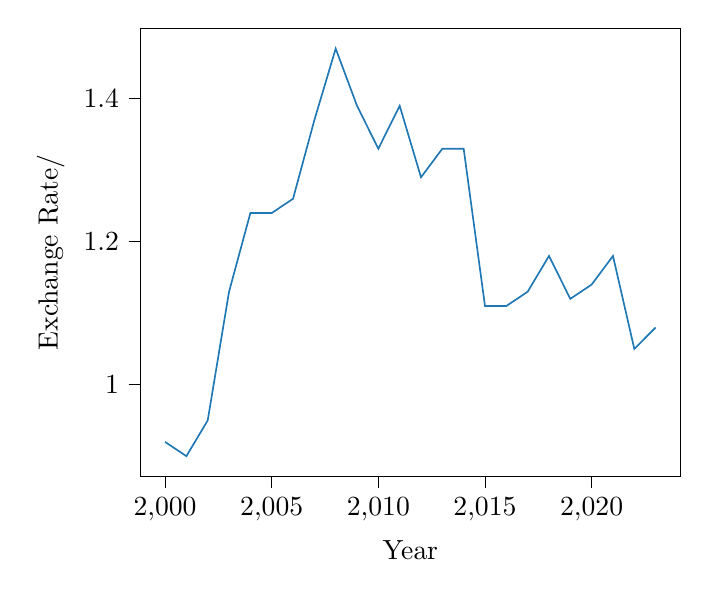
\begin{tikzpicture}

\definecolor{darkgray176}{RGB}{176,176,176}
\definecolor{steelblue31119180}{RGB}{31,119,180}

\begin{axis}[
tick align=outside,
tick pos=left,
x grid style={darkgray176},
xlabel={Year},
xmin=1998.85, xmax=2024.15,
xtick style={color=black},
y grid style={darkgray176},
ylabel={Exchange Rate/\unit{\USD\per\EUR}},
ymin=0.8715, ymax=1.4985,
ytick style={color=black}
]
\addplot [semithick, steelblue31119180]
table {%
2023 1.08
2022 1.05
2021 1.18
2020 1.14
2019 1.12
2018 1.18
2017 1.13
2016 1.11
2015 1.11
2014 1.33
2013 1.33
2012 1.29
2011 1.39
2010 1.33
2009 1.39
2008 1.47
2007 1.37
2006 1.26
2005 1.24
2004 1.24
2003 1.13
2002 0.95
2001 0.9
2000 0.92
};
\end{axis}

\end{tikzpicture}

        \caption{USD-EUR exchanger rate between 2002 and 2023 \cite{Macrotrends2024}}
        \label{fig:USD_EUR_exchange_rate}
    \end{figure}

    \begin{figure}[H]
        \centering
        % This file was created with tikzplotlib v0.10.1.
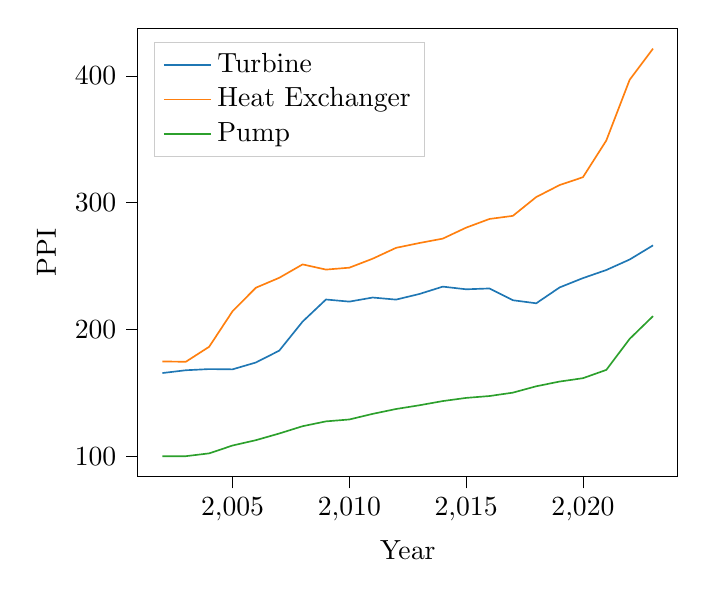
\begin{tikzpicture}

\definecolor{darkgray176}{RGB}{176,176,176}
\definecolor{darkorange25512714}{RGB}{255,127,14}
\definecolor{forestgreen4416044}{RGB}{44,160,44}
\definecolor{lightgray204}{RGB}{204,204,204}
\definecolor{steelblue31119180}{RGB}{31,119,180}

\begin{axis}[
legend cell align={left},
legend style={
  fill opacity=0.8,
  draw opacity=1,
  text opacity=1,
  at={(0.03,0.97)},
  anchor=north west,
  draw=lightgray204
},
tick align=outside,
tick pos=left,
x grid style={darkgray176},
xlabel={Year},
xmin=2000.95, xmax=2024.05,
xtick style={color=black},
y grid style={darkgray176},
ylabel={PPI},
ymin=83.92, ymax=437.68,
ytick style={color=black}
]
\addplot [semithick, steelblue31119180]
table {%
2002 165.6
2003 167.8
2004 168.72
2005 168.51
2006 173.92
2007 183.27
2008 206.19
2009 223.63
2010 221.96
2011 225.18
2012 223.54
2013 227.98
2014 233.78
2015 231.68
2016 232.34
2017 223.05
2018 220.63
2019 233.13
2020 240.5
2021 246.89
2022 255.18
2023 266.33
};
\addlegendentry{Turbine}
\addplot [semithick, darkorange25512714]
table {%
2002 174.75
2003 174.48
2004 186.33
2005 214.33
2006 232.92
2007 240.75
2008 251.32
2009 247.23
2010 248.73
2011 255.83
2012 264.39
2013 268.2
2014 271.66
2015 280.33
2016 287.18
2017 289.62
2018 304.47
2019 313.91
2020 320.12
2021 349.08
2022 397.02
2023 421.6
};
\addlegendentry{Heat Exchanger}
\addplot [semithick, forestgreen4416044]
table {%
2002 100
2003 100
2004 102.22
2005 108.41
2006 112.63
2007 117.89
2008 123.65
2009 127.46
2010 128.96
2011 133.39
2012 137.22
2013 140.17
2014 143.48
2015 145.98
2016 147.46
2017 150.13
2018 155.15
2019 158.88
2020 161.53
2021 168.08
2022 192.57
2023 210.51
};
\addlegendentry{Pump}
\end{axis}

\end{tikzpicture}

        \caption{PPI for turbines (WPU1197), heat exchangers (WPU1075) and pumps/compressors (PCU33391-33391) between 2002 and 2023 \cite{US_BLS2024}}
        \label{fig:PPI_correction}
    \end{figure}

    The \ac{NPV} can then be calculated using Equation~\ref{eq:economics_NPV}, where \(C_{rev_i}\) and \(C_{op_i}\) are the revenue and operating costs, calculated using Equations~\ref{eq:economics_revenue} and \ref{eq:economics_opcosts}, in year \(i\). \(f_{tax}\) is the tax rate, by default set at \qty{20}{\percent}, \(f_{disc\;rate}\) is the discount rate, by default set at \num{0.1}, \(f_{price}\) is the electricity price, by default set at \qty{0.4}{\USD\per\kWh}, and \(f_{inf}\) is the year on year rate of inflation, assumed to be \qty{3}{\percent}. \(C_{op_0}\) is the operating cost in year zero, which assumed to be \qty{5}{\percent} of the total plant cost \(C_{total}\).

    \begin{align}
        NPV = - C_{total} + \mathlarger{\sum}_{i=1}^N *\frac{(1-f_{tax})*(C_{rev_i} - C_{op_i})}{(1+f_{disc\;rate})^i}\label{eq:economics_NPV}
    \end{align}
    \begin{align}
        C_{rev_i} =  8.76*\Dot W_{elec}\cdot f_{price} \label{eq:economics_revenue}
    \end{align}
    \begin{align}
        C_{op_i} = C_{op_0} *(1+f_{inf})^i \label{eq:economics_opcosts}
    \end{align}

    Additional economic performance metrics are also calculated. The \ac{LCOE} is obtained by iteratively determining the price of electricity \(f_{price}\) for which the \ac{NPV} becomes zero. Similarly, the \ac{IRR} is found by determining the discount rate \(f_{disc\;rate}\) for which the \ac{NPV} becomes zero.

\section{Optimisation}
    The system performance can also be optimised. Here, a process metric (\emph{Objective Function}) is maximised/minimised, by adjusting process variables (\emph{Controls}), while ensuring that all process variables, parameters and metrics remain within their allowable range (\emph{Constraints}). In principle, any \emph{Objective Function}, \emph{Control} and \emph{Constraint} can be defined within \emph{PowerCycle}. 
    
    The optimisation is performed using \emph{pymoo} \cite{Blank2020}, an open-source framework for performing single and multi objective optimisation, and its \ac{GA}. While Newton and gradient-based optimisation algorithms, generally have a higher rate of convergence, requiring fewer iterations, obtaining derivatives can be computationally expensive, and require the \emph{Objective Function} to be calculable over the entire solution space, which may not be the case. \ac{GA}s on the other hand only require individual evaluations of the \emph{Objective Function}, allowing these to be parallelised, and non-calculable cases do not prevent the algorithm from proceeding.

\section{Validation}
    The following section provides a description of the validation of the various component models against their respective counterparts in \emph{Aspen Plus v11}. Validations for additional equipment is included in Appendix~\ref{ch:appendix_f}. 

    \subsection{Fluid Properties}
        \label{sec:PC_props_validation}
        The thermophysical properties calculations were validated by calculating relevant thermophysical properties (i.e. enthalpy, entropy and density) for a range of temperatures and pressures for several fluids. In \emph{Aspen Plus v11} this was achieved using an inlet stream, initialised to \qty{298}{K} and \qty{101325}{\Pa}, and a heater element to heat the fluid to the desired temperature and pressure, Figure~\ref{fig:Aspen_properties_validation}. \emph{REFPROP} was used as the property model for all fluids. A corresponding calculation was configured in \emph{PowerCycle}, see Listing~\ref{lst:PC_properties_validation}.

        \begin{figure}[H]
            \centering
            \includegraphics{Content/PowerCycle/Figures/AspenPlus_FluidPropertiesValidation.png}
            \caption{Process diagram of the \emph{Aspen Plus v11} simulation used to calculate the enthalpy, entropy and density of different fluids}
            \label{fig:Aspen_properties_validation}
        \end{figure}

        \begin{listing}[H]
            \caption{Configuration of a fluid properties calculation in \emph{PowerCycle} for water at a given temperature \(T\) and pressure \(P\)}
            \inputminted[bgcolor=bg,linenos, fontsize=\footnotesize]{python}{Content/PowerCycle/Code/FluidPropertiesComparison_snippet.py}
            \label{lst:PC_properties_validation}
            \vspace{-20pt}
        \end{listing}

        From Figure~\ref{fig:powercycle_val_water} it can be seen that the thermophysical properties calculated by \emph{Aspen Plus} and \emph{PowerCycle} are in close agreement, without any noticeable differences. Similar validation plots for n-butane and n-pentane, can be found in \nameref{ch:appendix_f}.   
        
        \begin{figure}[H]
            \centering
            % This file was created with tikzplotlib v0.10.1.
\begin{tikzpicture}

\definecolor{crimson2143940}{RGB}{214,39,40}
\definecolor{darkgray176}{RGB}{176,176,176}
\definecolor{darkorange25512714}{RGB}{255,127,14}
\definecolor{forestgreen4416044}{RGB}{44,160,44}
\definecolor{lightgray204}{RGB}{204,204,204}
\definecolor{mediumpurple148103189}{RGB}{148,103,189}
\definecolor{steelblue31119180}{RGB}{31,119,180}

\begin{groupplot}[group style={group size=1 by 3}]
\nextgroupplot[
tick align=outside,
tick pos=left,
x grid style={darkgray176},
xlabel={Temperature/K},
xmin=284.25, xmax=586.75,
xtick style={color=black},
y grid style={darkgray176},
ylabel={Enthalpy/J/kg},
ymin=-148498.207187226, ymax=3118435.34465385,
ytick style={color=black},
ytick={-2000000,0,2000000,4000000},
yticklabels={\ensuremath{-}2,0,2,4}
]
\addplot [semithick, steelblue31119180, mark=*, mark size=3, mark options={solid}, only marks]
table {%
298 -1.22755726
303.6122449 23460.4511
309.2244898 46916.2874
314.8367347 70371.8656
320.4489796 93831.4468
326.0612245 117298.454
331.6734694 140775.821
337.2857143 164266.246
342.8979592 187772.364
348.5102041 211296.875
354.122449 234842.625
359.7346939 258412.657
365.3469388 282010.25
370.9591837 305638.938
376.571429 2578551.65
382.183673 2590072.91
387.795918 2601503.9
393.408163 2612863.45
399.020408 2624165
404.632653 2635418.88
410.244898 2646633.45
415.857143 2657815.7
421.469388 2668971.57
427.081633 2680106.13
432.693878 2691223.8
438.306122 2702328.42
443.918367 2713423.34
449.530612 2724511.49
455.142857 2735595.46
460.755102 2746677.55
466.367347 2757759.78
471.979592 2768843.95
477.591837 2779931.67
483.204082 2791024.36
488.816327 2802123.32
494.428571 2813229.68
500.040816 2824344.5
505.653061 2835468.71
511.265306 2846603.15
516.877551 2857748.6
522.489796 2868905.76
528.102041 2880075.26
533.714286 2891257.69
539.326531 2902453.57
544.938776 2913663.4
550.55102 2924887.63
556.163265 2936126.68
561.77551 2947380.92
567.387755 2958650.71
573 2969936.39
};
\addplot [semithick, steelblue31119180]
table {%
298 -1.2275580863934
303.6122449 23460.4667807529
309.2244898 46916.3186999077
314.8367347 70371.912512831
320.4489796 93831.5093465216
326.0612245 117298.532017244
331.6734694 140775.914953586
337.2857143 164266.355050817
342.8979592 187772.488988366
348.5102041 211297.016069876
354.122449 234842.781157048
359.7346939 258412.828920894
365.3469388 282010.43804737
370.9591837 305639.14199851
376.571429 2578553.36879519
382.183673 2590074.63464815
387.795918 2601505.63122095
393.408163 2612865.19413648
399.020408 2624166.7475429
404.632653 2635420.63055021
410.244898 2646635.21239531
415.857143 2657817.47419529
421.469388 2668973.34502586
427.081633 2680107.91739338
432.693878 2691225.59839614
438.306122 2702330.22116953
443.918367 2713425.14185221
449.530612 2724513.29968866
455.142857 2735597.28418652
460.755102 2746679.38247807
466.367347 2757761.62074956
471.979592 2768845.79923413
477.591837 2779933.52190742
483.204082 2791026.22178783
488.816327 2802125.18256781
494.428571 2813231.55518854
500.040816 2824346.3817204
505.653061 2835470.59726347
511.265306 2846605.04977947
516.877551 2857750.50845271
522.489796 2868907.67268279
528.102041 2880077.17992583
533.714286 2891259.61254781
539.326531 2902455.50382836
544.938776 2913665.34323201
550.55102 2924889.57904469
556.163265 2936128.63046488
561.77551 2947382.87921564
567.387755 2958652.68073783
573 2969938.36502471
};
\addplot [semithick, darkorange25512714, mark=*, mark size=3, mark options={solid}, only marks]
table {%
298 199.080917
303.6122449 23657.3647
309.2244898 47110.0194
314.8367347 70562.5799
320.4489796 94019.2684
326.0612245 117483.476
331.6734694 140958.112
337.2857143 164445.852
342.8979592 187949.312
348.5102041 211471.176
354.122449 235014.273
359.7346939 258581.634
365.3469388 282176.523
370.9591837 305802.463
376.571429 329463.239
382.183673 353162.914
387.795918 376905.832
393.408163 400696.619
399.020408 424540.2
404.632653 448441.8
410.244898 2627015.65
415.857143 2639562.96
421.469388 2651903.54
427.081633 2664087.57
432.693878 2676146.34
438.306122 2688101.5
443.918367 2699969.35
449.530612 2711762.89
455.142857 2723492.89
460.755102 2735168.45
466.367347 2746797.41
471.979592 2758386.56
477.591837 2769941.84
483.204082 2781468.45
488.816327 2792970.98
494.428571 2804453.48
500.040816 2815919.56
505.653061 2827372.41
511.265306 2838814.9
516.877551 2850249.57
522.489796 2861678.73
528.102041 2873104.43
533.714286 2884528.54
539.326531 2895952.73
544.938776 2907378.53
550.55102 2918807.31
556.163265 2930240.34
561.77551 2941678.76
567.387755 2953123.63
573 2964575.89
};
\addplot [semithick, darkorange25512714]
table {%
298 198.870071259924
303.6122449 23657.1730435904
309.2244898 47109.8467849125
314.8367347 70562.426090556
320.4489796 94019.1332350799
326.0612245 117483.359771365
331.6734694 140958.014346615
337.2857143 164445.772074942
342.8979592 187949.250785155
348.5102041 211471.133064169
354.122449 235014.248591692
359.7346939 258581.627921156
365.3469388 282176.536309611
370.9591837 305802.494169545
376.571429 329463.29081899
382.183673 353162.981356334
387.795918 376905.918004399
393.408163 400696.725149054
399.020408 424540.325160014
404.632653 448441.944858426
410.244898 2627040.03026555
415.857143 2639585.39646113
421.469388 2651924.43201108
427.081633 2664107.16280619
432.693878 2676164.79769353
438.306122 2688118.95286543
443.918367 2699985.90696036
449.530612 2711778.63995856
455.142857 2723507.8993297
460.755102 2735182.78952239
466.367347 2746811.13483061
471.979592 2758399.7228564
477.591837 2769954.48070791
483.204082 2781480.60993522
488.816327 2792982.69395703
494.428571 2804464.78375153
500.040816 2815930.47889051
505.653061 2827382.97643571
511.265306 2838825.13088471
516.877551 2850259.49617096
522.489796 2861688.36331863
528.102041 2873113.79275495
533.714286 2884537.64213066
539.326531 2895961.5903454
544.938776 2907387.15835426
550.55102 2918815.72519743
556.163265 2930248.55187306
561.77551 2941686.78284252
567.387755 2953131.46617782
573 2964583.56204689
};
\addplot [semithick, forestgreen4416044, mark=*, mark size=3, mark options={solid}, only marks]
table {%
298 832.279824
303.6122449 24279.8621
309.2244898 47722.4864
314.8367347 71165.5317
320.4489796 94613.0978
326.0612245 118068.478
331.6734694 141534.5
337.2857143 165013.769
342.8979592 188508.846
348.5102041 212022.358
354.122449 235557.089
359.7346939 259116.025
365.3469388 282702.387
370.9591837 306319.657
376.571429 329971.58
382.183673 353662.178
387.795918 377395.752
393.408163 401176.886
399.020408 425010.456
404.632653 448901.64
410.244898 472855.931
415.857143 496879.156
421.469388 520977.501
427.081633 545157.538
432.693878 569426.266
438.306122 593791.153
443.918367 618260.191
449.530612 642841.962
455.142857 2678493.42
460.755102 2693129.84
466.367347 2707297.42
471.979592 2721122.31
477.591837 2734679.1
483.204082 2748016.33
488.816327 2761168.39
494.428571 2774161.48
500.040816 2787016.56
505.653061 2799750.99
511.265306 2812379.48
516.877551 2824914.7
522.489796 2837367.64
528.102041 2849747.93
533.714286 2862064.05
539.326531 2874323.48
544.938776 2886532.87
550.55102 2898698.16
556.163265 2910824.62
561.77551 2922917
567.387755 2934979.56
573 2947016.14
};
\addplot [semithick, forestgreen4416044]
table {%
298 832.280378689014
303.6122449 24279.8783191078
309.2244898 47722.5182373214
314.8367347 71165.5790841124
320.4489796 94613.1608375229
326.0612245 118068.55662703
331.6734694 141534.593929866
337.2857143 165013.879277051
342.8979592 188508.971137076
348.5102041 212022.499464626
354.122449 235557.24613719
359.7346939 259116.19726191
365.3469388 282702.575824454
370.9591837 306319.861167047
376.571429 329971.801907641
382.183673 353662.412083923
387.795918 377396.001811477
393.408163 401177.151686471
399.020408 425010.737954187
404.632653 448901.938311006
410.244898 472856.245835383
415.857143 496879.487603299
421.469388 520977.848697162
427.081633 545157.902326344
432.693878 569426.646852511
438.306122 593791.546302843
443.918367 618260.601597329
449.530612 642842.388760011
455.142857 2678495.20474186
460.755102 2693131.63765482
466.367347 2707299.2270643
471.979592 2721124.11950873
477.591837 2734680.92494883
483.204082 2748018.1579053
488.816327 2761170.23258511
494.428571 2774163.33077316
500.040816 2787018.41703466
505.653061 2799752.85401465
511.265306 2812381.35716423
516.877551 2824916.58409575
522.489796 2837369.53356684
528.102041 2849749.83279621
533.714286 2862065.95546553
539.326531 2874325.39362371
544.938776 2886534.79696356
550.55102 2898700.08563215
556.163265 2910826.5550527
561.77551 2922918.94409955
567.387755 2934981.51278961
573 2947018.09910582
};
\addplot [semithick, crimson2143940, mark=*, mark size=3, mark options={solid}, only marks]
table {%
298 2832.3173
303.6122449 26246.3992
309.2244898 49657.6063
314.8367347 73070.8345
320.4489796 96489.8045
326.0612245 119917.504
331.6734694 143356.508
337.2857143 166809.211
342.8979592 190277.987
348.5102041 213765.302
354.122449 237273.789
359.7346939 260806.297
365.3469388 284365.919
370.9591837 307956.004
376.571429 331580.176
382.183673 355242.327
387.795918 378946.628
393.408163 402697.528
399.020408 426499.761
404.632653 450358.354
410.244898 474278.637
415.857143 498266.26
421.469388 522327.216
427.081633 546467.868
432.693878 570694.978
438.306122 595015.755
443.918367 619437.898
449.530612 643969.658
455.142857 668619.906
460.755102 693398.217
466.367347 718314.967
471.979592 743381.451
477.591837 768610.021
483.204082 794014.258
488.816327 819609.178
494.428571 845411.478
500.040816 871439.851
505.653061 897715.374
511.265306 2703676.76
516.877551 2723240.53
522.489796 2741711.61
528.102041 2759375.53
533.714286 2776405.22
539.326531 2792915.01
544.938776 2808986.51
550.55102 2824681.55
556.163265 2840049.16
561.77551 2855129.45
567.387755 2869955.99
573 2884557.3
};
\addplot [semithick, crimson2143940]
table {%
298 2832.06258685984
303.6122449 26246.1643495965
309.2244898 49657.3910839368
314.8367347 73070.6387107605
320.4489796 96489.6279290683
326.0612245 119917.346478823
331.6734694 143356.369892557
337.2857143 166809.091798549
342.8979592 190277.886376128
348.5102041 213765.220180715
354.122449 237273.726713408
359.7346939 260806.254160866
365.3469388 284365.894392133
370.9591837 307955.999428457
376.571429 331580.191799612
382.183673 355242.358439164
387.795918 378946.679236845
393.408163 402697.599495583
399.020408 426499.853110855
404.632653 450358.46635252
410.244898 474278.769644677
415.857143 498266.413832947
421.469388 522327.391571718
427.081633 546468.064462032
432.693878 570695.196630643
438.306122 595015.99121672
443.918367 619438.156789783
449.530612 643969.939892881
455.142857 668620.211941404
460.755102 693398.54751944
466.367347 718315.32260127
471.979592 743381.831675647
477.591837 768610.428055804
483.204082 794014.692968891
488.816327 819609.640792846
494.428571 845411.965624531
500.040816 871440.370025011
505.653061 897715.924861783
511.265306 2703696.35004122
516.877551 2723258.41845852
522.489796 2741728.2006432
528.102041 2759391.06980465
533.714286 2776419.86881205
539.326531 2792928.8951716
544.938776 2808999.71178909
550.55102 2824694.14468704
556.163265 2840061.21211399
561.77551 2855141.01677188
567.387755 2869967.11258103
573 2884568.01651329
};
\addplot [semithick, mediumpurple148103189, mark=*, mark size=3, mark options={solid}, only marks]
table {%
298 9134.10495
303.6122449 32445.5819
309.2244898 55760.397
314.8367347 79082.0105
320.4489796 102413.013
326.0612245 125755.483
331.6734694 149111.242
337.2857143 172482.048
342.8979592 195869.726
348.5102041 219276.253
354.122449 242703.82
359.7346939 266154.864
365.3469388 289632.086
370.9591837 313138.458
376.571429 336677.228
382.183673 360251.912
387.795918 383866.296
393.408163 407524.431
399.020408 431230.632
404.632653 454989.483
410.244898 478805.84
415.857143 502684.842
421.469388 526631.924
427.081633 550652.839
432.693878 574753.681
438.306122 598940.912
443.918367 623221.405
449.530612 647602.48
455.142857 672091.963
460.755102 696698.242
466.367347 721430.343
471.979592 746298.01
477.591837 771311.812
483.204082 796483.258
488.816327 821824.941
494.428571 847350.71
500.040816 873075.876
505.653061 899017.466
511.265306 925194.537
516.877551 951628.558
522.489796 978343.903
528.102041 1005368.47
533.714286 1032734.49
539.326531 1060479.55
544.938776 1088648.05
550.55102 1117293.03
556.163265 1146478.91
561.77551 1176285.16
567.387755 1206811.93
573 1238188.48
};
\addplot [semithick, mediumpurple148103189]
table {%
298 9134.11103567471
303.6122449 32445.6034774607
309.2244898 55760.4341986775
314.8367347 79082.0632010597
320.4489796 102413.081579511
326.0612245 125755.566320415
331.6734694 149111.340895512
337.2857143 172482.163029961
342.8979592 195869.856323291
348.5102041 219276.39919069
354.122449 242703.982052125
359.7346939 266155.041553891
365.3469388 289632.278777777
370.9591837 313138.666856061
376.571429 336677.453819817
382.183673 360252.149952611
387.795918 383866.550255841
393.408163 407524.701347566
399.020408 431230.918999452
404.632653 454989.786254433
410.244898 478806.159233774
415.857143 502685.176949492
421.469388 526632.275553291
427.081633 550653.207429556
432.693878 574754.065563496
438.306122 598941.309366952
443.918367 623221.818462801
449.530612 647602.910512849
455.142857 672092.410252134
460.755102 696698.706367191
466.367347 721430.823625519
471.979592 746298.507973789
477.591837 771312.327189161
483.204082 796483.79040331
488.816327 821825.49078507
494.428571 847351.272386935
500.040816 873076.455809986
505.653061 899018.064039517
511.265306 925195.152309596
516.877551 951629.191330613
522.489796 978344.555060809
528.102041 1005369.14187235
533.714286 1032735.17642761
539.326531 1060480.26064784
544.938776 1088648.77480529
550.55102 1117293.77666525
556.163265 1146479.66824416
561.77551 1176285.93869443
567.387755 1206812.73239766
573 1238189.30636406
};

\nextgroupplot[
tick align=outside,
tick pos=left,
x grid style={darkgray176},
xlabel={Temperature/K},
xmin=284.25, xmax=586.75,
xtick style={color=black},
y grid style={darkgray176},
ylabel={Entropy/J/kg},
ymin=-395.294950179178, ymax=8244.23963920896,
ytick style={color=black}
]
\addplot [semithick, steelblue31119180, mark=*, mark size=3, mark options={solid}, only marks]
table {%
298 0.000339981509
303.6122449 77.9986647
309.2244898 154.54922
314.8367347 229.721997
320.4489796 303.579105
326.0612245 376.176826
331.6734694 447.56707
337.2857143 517.798427
342.8979592 586.9169
348.5102041 654.966433
354.122449 721.989278
359.7346939 788.026255
365.3469388 853.116931
370.9591837 917.299757
376.571429 7014.83099
382.183673 7045.20073
387.795918 7074.89317
393.408163 7103.97604
399.020408 7132.50049
404.632653 7160.50787
410.244898 7188.03297
415.857143 7215.1058
421.469388 7241.75265
427.081633 7267.99679
432.693878 7293.859
438.306122 7319.35793
443.918367 7344.51042
449.530612 7369.33176
455.142857 7393.8359
460.755102 7418.03561
466.367347 7441.94262
471.979592 7465.56779
477.591837 7488.92114
483.204082 7512.01203
488.816327 7534.84914
494.428571 7557.44062
500.040816 7579.79411
505.653061 7601.91677
511.265306 7623.81538
516.877551 7645.49632
522.489796 7666.96564
528.102041 7688.22907
533.714286 7709.29207
539.326531 7730.15982
544.938776 7750.83727
550.55102 7771.32913
556.163265 7791.63994
561.77551 7811.77399
567.387755 7831.73545
573 7851.52829
};
\addplot [semithick, steelblue31119180]
table {%
298 0.000339981943511702
303.6122449 77.9987166831037
309.2244898 154.549323218255
314.8367347 229.722149736493
320.4489796 303.579307351125
326.0612245 376.177076292281
331.6734694 447.567368653518
337.2857143 517.798772043611
342.8979592 586.917290762874
348.5102041 654.966869136519
354.122449 721.989759384547
359.7346939 788.026780161389
365.3469388 853.11749975097
370.9591837 917.300368756212
376.571429 7014.83566534461
382.183673 7045.20541731615
387.795918 7074.89788133581
393.408163 7103.98076831736
399.020408 7132.50524270301
404.632653 7160.51264235907
410.244898 7188.0377595118
415.857143 7215.11060604581
421.469388 7241.75747310588
427.081633 7268.00163610431
432.693878 7293.86386399493
438.306122 7319.36280450836
443.918367 7344.51531193975
449.530612 7369.33667186618
455.142857 7393.84082756409
460.755102 7418.04054923403
466.367347 7441.94758020618
471.979592 7465.5727606785
477.591837 7488.92613298071
483.204082 7512.01703153734
488.816327 7534.85416008529
494.428571 7557.44565421931
500.040816 7579.79915503111
505.653061 7601.92183497203
511.265306 7623.8204575979
516.877551 7645.5014116716
522.489796 7666.97074466137
528.102041 7688.23419225673
533.714286 7709.29720446331
539.326531 7730.16496874908
544.938776 7750.84243064078
550.55102 7771.33430847354
556.163265 7791.64512442277
561.77551 7811.77919737755
567.387755 7831.74067088689
573 7851.5335215095
};
\addplot [semithick, darkorange25512714, mark=*, mark size=3, mark options={solid}, only marks]
table {%
298 -0.0551653682
303.6122449 77.9318716
309.2244898 154.472043
314.8367347 229.635147
320.4489796 303.483148
326.0612245 376.072209
331.6734694 447.454148
337.2857143 517.677477
342.8979592 586.788134
348.5102041 654.830008
354.122449 721.845304
359.7346939 787.874796
365.3469388 852.958015
370.9591837 917.133374
376.571429 980.438273
382.183673 1042.90917
387.795918 1104.58167
393.408163 1165.49056
399.020408 1225.6699
404.632653 1285.15307
410.244898 6618.71758
415.857143 6649.09585
421.469388 6678.57292
427.081633 6707.29097
432.693878 6735.34262
438.306122 6762.7948
443.918367 6789.69974
449.530612 6816.10028
455.142857 6842.03275
460.755102 6867.52851
466.367347 6892.61505
471.979592 6917.31663
477.591837 6941.65486
483.204082 6965.64906
488.816327 6989.31662
494.428571 7012.67326
500.040816 7035.73322
505.653061 7058.5095
511.265306 7081.01398
516.877551 7103.25757
522.489796 7125.25033
528.102041 7147.00152
533.714286 7168.51977
539.326531 7189.81307
544.938776 7210.8889
550.55102 7231.75423
556.163265 7252.41562
561.77551 7272.87919
567.387755 7293.15076
573 7313.23578
};
\addplot [semithick, darkorange25512714]
table {%
298 -0.0551069125806976
303.6122449 77.9319939460611
309.2244898 154.472227245274
314.8367347 229.635391883431
320.4489796 303.483451470588
326.0612245 376.07256990565
331.6734694 447.454565586426
337.2857143 517.677949109243
342.8979592 586.788660192269
348.5102041 654.830587906524
354.122449 721.845936233544
359.7346939 787.87548084856
365.3469388 852.958750954651
370.9591837 917.134160892267
376.571429 980.439113886468
382.183673 1042.91005379744
387.795918 1104.58260233188
393.408163 1165.49154233567
399.020408 1225.67093067077
404.632653 1285.15415478295
410.244898 6619.09900527373
415.857143 6649.47257046048
421.469388 6678.94594117181
427.081633 6707.66091688682
432.693878 6735.70993428702
438.306122 6763.15981308538
443.918367 6790.06271454956
449.530612 6816.46144600256
455.142857 6842.39228380871
460.755102 6867.88658155745
466.367347 6892.9717916596
471.979592 6917.67217116107
477.591837 6942.0093040781
483.204082 6966.00250728305
488.816327 6989.66915632762
494.428571 7013.02494846353
500.040816 7036.08414137379
505.653061 7058.85971470946
511.265306 7081.36354448298
516.877551 7103.60653296032
522.489796 7125.59872319757
528.102041 7147.34939728594
533.714286 7168.867160941
539.326531 7190.16001659284
544.938776 7211.2354267539
550.55102 7232.10036543759
556.163265 7252.7613810855
561.77551 7273.22461635692
567.387755 7293.49585998988
573 7313.58057560176
};
\addplot [semithick, forestgreen4416044, mark=*, mark size=3, mark options={solid}, only marks]
table {%
298 -0.230999382
303.6122449 77.7204567
309.2244898 154.22789
314.8367347 229.360496
320.4489796 303.179776
326.0612245 375.741526
331.6734694 447.09727
337.2857143 517.295276
342.8979592 586.381279
348.5102041 654.398996
354.122449 721.390478
359.7346939 787.396365
365.3469388 852.456064
370.9591837 916.607875
376.571429 979.889087
382.183673 1042.33606
387.795918 1103.98429
393.408163 1164.86846
399.020408 1225.02254
404.632653 1284.47979
410.244898 1343.27291
415.857143 1401.43403
421.469388 1458.9949
427.081633 1515.98686
432.693878 1572.44107
438.306122 1628.38852
443.918367 1683.86024
449.530612 1738.88738
455.142857 6232.42397
460.755102 6264.38643
466.367347 6294.95013
471.979592 6324.41758
477.591837 6352.97192
483.204082 6380.73551
488.816327 6407.79744
494.428571 6434.22702
500.040816 6460.08067
505.653061 6485.40581
511.265306 6510.24303
516.877551 6534.62762
522.489796 6558.59053
528.102041 6582.15909
533.714286 6605.35761
539.326531 6628.20779
544.938776 6650.72911
550.55102 6672.93913
556.163265 6694.85372
561.77551 6716.4873
567.387755 6737.853
573 6758.96283
};
\addplot [semithick, forestgreen4416044]
table {%
298 -0.230999535999047
303.6122449 77.7205085376295
309.2244898 154.227992499774
314.8367347 229.360649265595
320.4489796 303.179978064888
326.0612245 375.741776494069
331.6734694 447.09756788891
337.2857143 517.29562030134
342.8979592 586.381670044973
348.5102041 654.399432160429
354.122449 721.390958699888
359.7346939 787.396889983761
365.3469388 852.456632149995
370.9591837 916.608485368707
376.571429 979.889744830807
382.183673 1042.33675020928
387.795918 1103.98502086375
393.408163 1164.86923739908
399.020408 1225.02335289067
404.632653 1284.48064788524
410.244898 1343.27380164064
415.857143 1401.43496986548
421.469388 1458.9958701296
427.081633 1515.9878760292
432.693878 1572.44212126571
438.306122 1628.38960508968
443.918367 1683.86136047358
449.530612 1738.88853793705
455.142857 6232.4281162405
460.755102 6264.39059878625
466.367347 6294.95432611553
471.979592 6324.42179663052
477.591837 6352.9761523741
483.204082 6380.73975870556
488.816327 6407.80171169259
494.428571 6434.23130183993
500.040816 6460.08497624649
505.653061 6485.4101262721
511.265306 6510.24736609397
516.877551 6534.63197561145
522.489796 6558.59489891929
528.102041 6582.16347674628
533.714286 6605.3620095617
539.326531 6628.21220527535
544.938776 6650.73354355882
550.55102 6672.94357319003
556.163265 6694.85817981296
561.77551 6716.49177472673
567.387755 6737.85749118105
573 6758.96733435048
};
\addplot [semithick, crimson2143940, mark=*, mark size=3, mark options={solid}, only marks]
table {%
298 -0.790130433
303.6122449 77.0499414
309.2244898 153.454832
314.8367347 228.491872
320.4489796 302.221118
326.0612245 374.697231
331.6734694 445.970818
337.2857143 516.089393
342.8979592 585.09806
348.5102041 653.039994
354.122449 719.956774
359.7346939 785.888621
365.3469388 850.874558
370.9591837 914.95253
376.571429 978.159494
382.183673 1040.53149
387.795918 1102.10368
393.408163 1162.91045
399.020408 1222.98544
404.632653 1282.36159
410.244898 1341.07124
415.857143 1399.14618
421.469388 1456.61774
427.081633 1513.51688
432.693878 1569.87428
438.306122 1625.72045
443.918367 1681.08586
449.530612 1736.00106
455.142857 1790.49683
460.755102 1844.60435
466.367347 1898.35542
471.979592 1951.78262
477.591837 2004.91964
483.204082 2057.80152
488.816327 2110.46505
494.428571 2162.94918
500.040816 2215.29554
505.653061 2267.54912
511.265306 5809.20269
516.877551 5847.26186
522.489796 5882.80673
528.102041 5916.43487
533.714286 5948.51263
539.326531 5979.28567
544.938776 6008.93152
550.55102 6037.58624
556.163265 6065.35854
561.77551 6092.33792
567.387755 6118.59959
573 6144.20773
};
\addplot [semithick, crimson2143940]
table {%
298 -0.790058860248507
303.6122449 77.0500790419415
309.2244898 153.455033772736
314.8367347 228.49213544922
320.4489796 302.221442281261
326.0612245 374.697614633208
331.6734694 445.971259447559
337.2857143 516.089891291404
342.8979592 585.098614484645
348.5102041 653.040603314956
354.122449 719.957437785131
359.7346939 785.889337746677
365.3469388 850.875327177987
370.9591837 914.953351888946
376.571429 978.160371980665
382.183673 1040.5324042378
387.795918 1102.10465115055
393.408163 1162.91147714642
399.020408 1222.98651475434
404.632653 1282.36271482265
410.244898 1341.0724129835
415.857143 1399.14740246478
421.469388 1456.61901425003
427.081633 1513.51820548963
432.693878 1569.87565712336
438.306122 1625.72187195137
443.918367 1681.08733412952
449.530612 1736.00258293959
455.142857 1790.49840226972
460.755102 1844.60597951249
466.367347 1898.35709788296
471.979592 1951.7843575175
477.591837 2004.92143233138
483.204082 2057.80337177002
488.816327 2110.4669595003
494.428571 2162.95113573506
500.040816 2215.29756081061
505.653061 2267.55120922828
511.265306 5809.27586634518
516.877551 5847.3317413483
522.489796 5882.87411438038
528.102041 5916.50023940157
533.714286 5948.57633143251
539.326531 5979.34792986842
544.938776 6008.99253620308
550.55102 6037.64614683878
556.163265 6065.41746587574
561.77551 6092.39596798305
567.387755 6118.65685699272
573 6144.26428020594
};
\addplot [semithick, mediumpurple148103189, mark=*, mark size=3, mark options={solid}, only marks]
table {%
298 -2.58883076
303.6122449 74.9100947
309.2244898 151.000373
314.8367347 225.743777
320.4489796 299.196064
326.0612245 371.408497
331.6734694 442.428944
337.2857143 512.302661
342.8979592 581.072862
348.5102041 648.781101
354.122449 715.467543
359.7346939 781.17115
365.3469388 845.929803
370.9591837 909.780389
376.571429 972.758864
382.183673 1034.9003
387.795918 1096.23895
393.408163 1156.80823
399.020408 1216.64085
404.632653 1275.76879
410.244898 1334.22337
415.857143 1392.03535
421.469388 1449.23492
427.081633 1505.85186
432.693878 1561.91555
438.306122 1617.45509
443.918367 1672.4994
449.530612 1727.07731
455.142857 1781.21768
460.755102 1834.94957
466.367347 1888.30233
471.979592 1941.3058
477.591837 1993.99051
483.204082 2046.38784
488.816327 2098.53036
494.428571 2150.45204
500.040816 2202.18866
505.653061 2253.77821
511.265306 2305.26142
516.877551 2356.68237
522.489796 2408.08929
528.102041 2459.5356
533.714286 2511.08116
539.326531 2562.79395
544.938776 2614.75238
550.55102 2667.04827
556.163265 2719.79112
561.77551 2773.11415
567.387755 2827.18318
573 2882.21015
};
\addplot [semithick, mediumpurple148103189]
table {%
298 -2.58883247971755
303.6122449 74.9101445860753
309.2244898 151.000473932854
314.8367347 225.743927050884
320.4489796 299.196263133424
326.0612245 371.408744888213
331.6734694 442.429238377762
337.2857143 512.303002736577
342.8979592 581.073249537403
348.5102041 648.781533221977
354.122449 715.468019912851
359.7346939 781.171670700911
365.3469388 845.930366550405
370.9591837 909.780994884571
376.571429 972.759516869029
382.183673 1034.90098903796
387.795918 1096.23967424766
393.408163 1156.80900249061
399.020408 1216.64166252366
404.632653 1275.7696385104
410.244898 1334.22426308897
415.857143 1392.03627653052
421.469388 1449.23589252933
427.081633 1505.85287105757
432.693878 1561.91659873577
438.306122 1617.45616743395
443.918367 1672.50051106532
449.530612 1727.07845342158
455.142857 1781.21886636541
460.755102 1834.95079160067
466.367347 1888.30358802864
471.979592 1941.3070979294
477.591837 1993.9918360745
483.204082 2046.38920707322
488.816327 2098.53175781247
494.428571 2150.45346468208
500.040816 2202.19012271264
505.653061 2253.77971342403
511.265306 2305.26295704922
516.877551 2356.68393823777
522.489796 2408.09089915156
528.102041 2459.53724407919
533.714286 2511.08283125163
539.326531 2562.7956612522
544.938776 2614.75412369033
550.55102 2667.05003784152
556.163265 2719.79292574755
561.77551 2773.11599543669
567.387755 2827.18505859505
573 2882.21207448056
};

\nextgroupplot[
legend cell align={left},
legend style={
  fill opacity=0.8,
  draw opacity=1,
  text opacity=1,
  at={(0.97,0.03)},
  anchor=south east,
  draw=lightgray204
},
tick align=outside,
tick pos=left,
unbounded coords=jump,
x grid style={darkgray176},
xlabel={Temperature/K},
xmin=284.25, xmax=586.75,
xtick style={color=black},
y grid style={darkgray176},
ylabel={Density/kg/m3},
ymin=-49.6773840421895, ymax=1051.56424781153,
ytick style={color=black}
]
\addplot [semithick, black, mark=*, mark size=3, mark options={solid}, only marks]
table {%
nan nan
nan nan
};
\addlegendentry{AspenPlus}
\addplot [semithick, black]
table {%
nan nan
nan nan
};
\addlegendentry{PowerCycle}
\addplot [semithick, steelblue31119180]
table {%
nan nan
nan nan
};
\addlegendentry{\qty{1.00}{\bar}}
\addplot [semithick, darkorange25512714]
table {%
nan nan
nan nan
};
\addlegendentry{\qty{3.16}{\bar}}
\addplot [semithick, forestgreen4416044]
table {%
nan nan
nan nan
};
\addlegendentry{\qty{10.00}{\bar}}
\addplot [semithick, crimson2143940]
table {%
nan nan
nan nan
};
\addlegendentry{\qty{31.62}{\bar}}
\addplot [semithick, mediumpurple148103189]
table {%
nan nan
nan nan
};
\addlegendentry{\qty{100.00}{\bar}}
\addplot [semithick, steelblue31119180, mark=*, mark size=3, mark options={solid}, only marks, forget plot]
table {%
298 997.086075
303.6122449 995.508975
309.2244898 993.659344
314.8367347 991.560774
320.4489796 989.23261
326.0612245 986.690894
331.6734694 983.949048
337.2857143 981.018372
342.8979592 977.908429
348.5102041 974.627332
354.122449 971.181963
359.7346939 967.578144
365.3469388 963.820775
370.9591837 959.913932
376.571429 0.583891623
382.183673 0.574700222
387.795918 0.565839995
393.408163 0.55728692
399.020408 0.549020594
404.632653 0.541023181
410.244898 0.533278823
415.857143 0.525773264
421.469388 0.518493595
427.081633 0.511428056
432.693878 0.504565882
438.306122 0.497897177
443.918367 0.491412811
449.530612 0.485104332
455.142857 0.478963891
460.755102 0.472984181
466.367347 0.467158381
471.979592 0.461480108
477.591837 0.455943378
483.204082 0.45054257
488.816327 0.445272393
494.428571 0.440127858
500.040816 0.435104255
505.653061 0.430197133
511.265306 0.425402273
516.877551 0.420715679
522.489796 0.416133558
528.102041 0.411652303
533.714286 0.407268486
539.326531 0.402978844
544.938776 0.398780264
550.55102 0.394669781
556.163265 0.390644561
561.77551 0.386701901
567.387755 0.382839212
573 0.379054022
};
\addplot [semithick, steelblue31119180, forget plot]
table {%
298 997.085410835717
303.6122449 995.508311906078
309.2244898 993.658682289052
314.8367347 991.560113156837
320.4489796 989.231950816091
326.0612245 986.690237209797
331.6734694 983.948392238154
337.2857143 981.017718085838
342.8979592 977.907777814422
348.5102041 974.626683248729
354.122449 971.181316206272
359.7346939 967.577499917741
365.3469388 963.82013264274
370.9591837 959.913292153242
376.571429 0.583891233208001
382.183673 0.574699839636566
387.795918 0.565839619147328
393.408163 0.557286549475379
399.020408 0.549020228732728
404.632653 0.541022821091274
410.244898 0.533278467362627
415.857143 0.525772913174118
421.469388 0.518493249048296
427.081633 0.511427714834872
432.693878 0.504565545364488
438.306122 0.497896846107139
443.918367 0.491412484415452
449.530612 0.485104009283203
455.142857 0.478963572480164
460.755102 0.472983866457594
466.367347 0.467158069900331
471.979592 0.461479800613977
477.591837 0.455943074535561
483.204082 0.450542269888973
488.816327 0.445272095687935
494.428571 0.440127564838369
500.040816 0.435103965844943
505.653061 0.43019684636694
511.265306 0.425401989920581
516.877551 0.420715399217547
522.489796 0.416133280333007
528.102041 0.411652028408294
533.714286 0.407268214699212
539.326531 0.402978574808796
544.938776 0.3987799979665
550.55102 0.394669517959907
556.163265 0.390644301253183
561.77551 0.386701643149802
567.387755 0.382838957276329
573 0.379053769343343
};
\addplot [semithick, darkorange25512714, mark=*, mark size=3, mark options={solid}, only marks, forget plot]
table {%
298 997.183639
303.6122449 995.605244
309.2244898 993.754687
314.8367347 991.65551
320.4489796 989.327023
326.0612245 986.785236
331.6734694 984.043548
337.2857143 981.113241
342.8979592 978.003865
348.5102041 974.723521
354.122449 971.279084
359.7346939 967.67637
365.3469388 963.920275
370.9591837 960.014875
376.571429 955.963511
382.183673 951.768847
387.795918 947.432925
393.408163 942.957198
399.020408 938.342558
404.632653 933.589351
410.244898 1.72567406
415.857143 1.69863
421.469388 1.67270861
427.081633 1.64779273
432.693878 1.62379392
438.306122 1.60064058
443.918367 1.57827217
449.530612 1.5566362
455.142857 1.53568635
460.755102 1.51538135
466.367347 1.49568412
471.979592 1.47656115
477.591837 1.45798197
483.204082 1.43991877
488.816327 1.42234607
494.428571 1.40524044
500.040816 1.38858022
505.653061 1.3723454
511.265306 1.35651738
516.877551 1.34107883
522.489796 1.32601359
528.102041 1.31130656
533.714286 1.29694356
539.326531 1.28291129
544.938776 1.26919722
550.55102 1.25578955
556.163265 1.24267715
561.77551 1.22984948
567.387755 1.21729656
573 1.20500895
};
\addplot [semithick, darkorange25512714, forget plot]
table {%
298 997.182871900019
303.6122449 995.604478976757
309.2244898 993.753924201489
314.8367347 991.65474981225
320.4489796 989.326264178803
326.0612245 986.784479598511
331.6734694 984.04279274061
337.2857143 981.112487637078
342.8979592 978.003113302513
348.5102041 974.722770901791
354.122449 971.278334443502
359.7346939 967.675621798931
365.3469388 963.91952801904
370.9591837 960.014129598699
376.571429 955.962765712742
382.183673 951.768103511306
387.795918 947.432182394185
393.408163 942.956456113212
399.020408 938.341816035328
404.632653 933.588609401369
410.244898 1.72438470791264
415.857143 1.69736449067032
421.469388 1.6714654132611
427.081633 1.64657062263568
432.693878 1.62259185684379
438.306122 1.59945764070986
443.918367 1.577107534333
449.530612 1.55548910662879
455.142857 1.53455611836226
460.755102 1.51426735092068
466.367347 1.49458577111536
471.979592 1.47547789959728
477.591837 1.45691331265222
483.204082 1.438864238172
488.816327 1.42130522192488
494.428571 1.4042128513621
500.040816 1.38756550772489
505.653061 1.37134318367421
511.265306 1.35552729922111
516.877551 1.34010055686237
522.489796 1.32504681351959
528.102041 1.31035096916265
533.714286 1.29599886950557
539.326531 1.28197722063139
544.938776 1.26827351377617
550.55102 1.25487596116452
556.163265 1.24177342745636
561.77551 1.22895539144812
567.387755 1.21641188942979
573 1.20413347540526
};
\addplot [semithick, forestgreen4416044, mark=*, mark size=3, mark options={solid}, only marks, forget plot]
table {%
298 997.491869
303.6122449 995.90938
309.2244898 994.055894
314.8367347 991.954799
320.4489796 989.625284
326.0612245 987.083267
331.6734694 984.342071
337.2857143 981.412923
342.8979592 978.305328
348.5102041 975.027352
354.122449 971.585846
359.7346939 967.98661
365.3469388 964.234528
370.9591837 960.333674
376.571429 956.287388
382.183673 952.098342
387.795918 947.76859
393.408163 943.299601
399.020408 938.692288
404.632653 933.947027
410.244898 929.063662
415.857143 924.041513
421.469388 918.879367
427.081633 913.57547
432.693878 908.127506
438.306122 902.532572
443.918367 896.787142
449.530612 890.887023
455.142857 5.11157713
460.755102 5.02647559
466.367347 4.94597392
471.979592 4.86938713
477.591837 4.79624062
483.204082 4.7261768
488.816327 4.65890986
494.428571 4.59420235
500.040816 4.53185191
505.653061 4.47168318
511.265306 4.41354241
516.877551 4.35729362
522.489796 4.30281567
528.102041 4.25000001
533.714286 4.1987489
539.326531 4.1489739
544.938776 4.10059466
550.55102 4.05353788
556.163265 4.00773649
561.77551 3.96312887
567.387755 3.91965827
573 3.87727224
};
\addplot [semithick, forestgreen4416044, forget plot]
table {%
298 997.491204743459
303.6122449 995.908716584422
309.2244898 994.055231879167
314.8367347 991.954138352954
320.4489796 989.624624529871
326.0612245 987.082609010957
331.6734694 984.341415008978
337.2857143 981.412269126171
342.8979592 978.3046759069
348.5102041 975.026702737382
354.122449 971.585198845593
359.7346939 967.985965051992
365.3469388 964.233886140571
370.9591837 960.33303442907
376.571429 956.286750513216
382.183673 952.097708234851
387.795918 947.767958780692
393.408163 943.298972724129
399.020408 938.691663358034
404.632653 933.94640513385
410.244898 929.06304348469
415.857143 924.040897345931
421.469388 918.878754662531
427.081633 913.574860909207
432.693878 908.126900396347
438.306122 902.531970885506
443.918367 896.786544711234
449.530612 890.88643033397
455.142857 5.11157372748583
460.755102 5.02647224272531
466.367347 4.94597062917312
471.979592 4.86938388475276
477.591837 4.79623742021247
483.204082 4.72617364258968
488.816327 4.65890675432384
494.428571 4.59419929704343
500.040816 4.53184889213317
505.653061 4.47168020009255
511.265306 4.41353947386765
516.877551 4.35729071923405
522.489796 4.30281279994365
528.102041 4.24999717822361
533.714286 4.19874610411213
539.326531 4.14897113740837
544.938776 4.100591924916
550.55102 4.05353518688691
556.163265 4.00773382290506
561.77551 3.96312623210466
567.387755 3.91965565657972
573 3.87726965573098
};
\addplot [semithick, crimson2143940, mark=*, mark size=3, mark options={solid}, only marks, forget plot]
table {%
298 998.463653
303.6122449 996.868243
309.2244898 995.005493
314.8367347 992.898307
320.4489796 990.565498
326.0612245 988.02269
331.6734694 985.282975
337.2857143 982.357399
342.8979592 979.255326
348.5102041 975.984716
354.122449 972.552339
359.7346939 968.963943
365.3469388 965.224377
370.9591837 961.3377
376.571429 957.307256
382.183673 953.135737
387.795918 948.82523
393.408163 944.377256
399.020408 939.792794
404.632653 935.072303
410.244898 930.215725
415.857143 925.2225
421.469388 920.091552
427.081633 914.821286
432.693878 909.409573
438.306122 903.853721
443.918367 898.150449
449.530612 892.295847
455.142857 886.285325
460.755102 880.113553
466.367347 873.774387
471.979592 867.260775
477.591837 860.56465
483.204082 853.676789
488.816327 846.586648
494.428571 839.282149
500.040816 831.749424
505.653061 823.972483
511.265306 15.7336043
516.877551 15.4026862
522.489796 15.0986992
528.102041 14.8164905
533.714286 14.5525657
539.326531 14.30437
544.938776 14.0699336
550.55102 13.8476796
556.163265 13.6363132
561.77551 13.4347506
567.387755 13.2420727
573 13.0574911
};
\addplot [semithick, crimson2143940, forget plot]
table {%
298 998.462863580588
303.6122449 996.867455912107
309.2244898 995.004708433794
314.8367347 992.897524918994
320.4489796 990.56471795097
326.0612245 988.021911795957
331.6734694 985.282198573025
337.2857143 982.356623911356
342.8979592 979.254551929575
348.5102041 975.983943042374
354.122449 972.551567653545
359.7346939 968.963171921611
365.3469388 965.223607150608
370.9591837 961.336931163563
376.571429 957.306487479551
382.183673 953.13496922518
387.795918 948.824462647091
393.408163 944.376488920922
399.020408 939.792027651654
404.632653 935.071535817578
410.244898 930.214958457912
415.857143 925.221732433449
421.469388 920.090783584029
427.081633 914.820517360917
432.693878 909.408802779918
438.306122 903.852950309397
443.918367 898.149677062424
449.530612 892.295073282206
455.142857 886.2845490659
460.755102 880.112774440826
466.367347 873.773604719357
471.979592 867.259989257685
477.591837 860.563859893032
483.204082 853.675994169534
488.816327 846.585846886976
494.428571 839.281342662785
500.040816 831.74860996944
505.653061 823.971660328153
511.265306 15.7319001709238
516.877551 15.4010473955903
522.489796 15.0971159603537
528.102041 14.814956000095
533.714286 14.5510746067404
539.326531 14.3029182629358
544.938776 14.0685176762777
550.55102 13.8462967152289
556.163265 13.6349607148212
561.77551 13.433426509401
567.387755 13.2407750990881
573 13.0562182668176
};
\addplot [semithick, mediumpurple148103189, mark=*, mark size=3, mark options={solid}, only marks, forget plot]
table {%
298 1001.50781
303.6122449 999.871809
309.2244898 997.979772
314.8367347 995.853115
320.4489796 993.50949
326.0612245 990.963611
331.6734694 988.227848
337.2857143 985.312681
342.8979592 982.227032
348.5102041 978.978522
354.122449 975.573667
359.7346939 972.018034
365.3469388 968.316359
370.9591837 964.472643
376.571429 960.490223
382.183673 956.371836
387.795918 952.11966
393.408163 947.735352
399.020408 943.220074
404.632653 938.574513
410.244898 933.798891
415.857143 928.892975
421.469388 923.856078
427.081633 918.687052
432.693878 913.384281
438.306122 907.945669
443.918367 902.368614
449.530612 896.649982
455.142857 890.786079
460.755102 884.772601
466.367347 878.604588
471.979592 872.276361
477.591837 865.781441
483.204082 859.112468
488.816327 852.261077
494.428571 845.217773
500.040816 837.971759
505.653061 830.510731
511.265306 822.820628
516.877551 814.885306
522.489796 806.686137
528.102041 798.20149
533.714286 789.406054
539.326531 780.269954
544.938776 770.75756
550.55102 760.825859
556.163265 750.422189
561.77551 739.480984
567.387755 727.918964
573 715.627759
};
\addplot [semithick, mediumpurple148103189, forget plot]
table {%
298 1001.50714350671
303.6122449 999.871143278598
309.2244898 997.979106874195
314.8367347 995.852451267508
320.4489796 993.508828597005
326.0612245 990.962950550455
331.6734694 988.227189523801
337.2857143 985.312024692735
342.8979592 982.226377916246
348.5102041 978.977869861562
354.122449 975.573017369897
359.7346939 972.01738687418
365.3469388 968.315714472532
370.9591837 964.472000349529
376.571429 960.489582897014
382.183673 956.371199099158
387.795918 952.119025917968
393.408163 947.734721009649
399.020408 943.219446295997
404.632653 938.57388793472
410.244898 933.798269036989
415.857143 928.892356484092
421.469388 923.855462239564
427.081633 918.686439352041
432.693878 913.383672662163
438.306122 907.945065033598
443.918367 902.368012907165
449.530612 896.649385245278
455.142857 890.785485744489
460.755102 884.772011794214
466.367347 878.604003113948
471.979592 872.275779341183
477.591837 865.780864398941
483.204082 859.111894843195
488.816327 852.260508565129
494.428571 845.217210398514
500.040816 837.971200831775
505.653061 830.510178510855
511.265306 822.820080423545
516.877551 814.884763548324
522.489796 806.68559994389
528.102041 798.20095778489
533.714286 789.405527497224
539.326531 780.26943377325
544.938776 770.757045676958
550.55102 760.825353146697
556.163265 750.421690048373
561.77551 739.480491619378
567.387755 727.918478902401
573 715.627282354213
};
\end{groupplot}

\end{tikzpicture}

            \caption[Comparison of the thermophysical properties of water calculated by \emph{Aspen Plus} and \emph{PowerCycle}.]{Comparison of the thermophysical properties of water calculated by \emph{Aspen Plus} and \emph{PowerCycle}. The enthalpy and entropy are reported relative to \qty{298}{\K} and \qty{101325}{\Pa}}
            \label{fig:powercycle_val_water}
        \end{figure}

    \subsection{Turbine}
        \label{sec:PC_dry_turbine_validation}
        A stream of saturated steam at a temperature of \qty{473}{\K} (\qty{200}{\degreeCelsius}) was expanded in a turbine to a discharge pressure of \qty{0.1}{\bar}. The expansion process is assumed to be dry (i.e. wetness effects are negligible), with the isentropic efficiency of the turbine being \qty{85}{\percent} and the efficiency of the generator being \qty{95}{\percent} respectively, see Table~\ref{table:turbine_dry_validation_inputs}.

        \begin{table}[H]
            \caption{The boundary conditions for the turbine performance validation calculations for a dry expansion}
            \centering 
            \label{table:turbine_dry_validation_inputs}
            \input{Content/PowerCycle/DataTables/TurbineValidation/Dry_inputs}        
        \end{table}

        Models for each scenario were then formulated in \emph{AspenPlus v11} and \emph{PowerCycle}, Figure~\ref{fig:Aspen_turb_dry_validation} and Listing~\ref{lst:PC_turbine_dry_validation} respectively.

        \begin{figure}[H]
            \centering
            \includegraphics{Content/PowerCycle/Figures/AspenPlus_TurbineDryValidation.png}
            \caption{Process diagram of the \emph{Aspen Plus v11} simulation used to calculate the performance of a turbine, assuming dry expansion}
            \label{fig:Aspen_turb_dry_validation}
        \end{figure}

        \begin{listing}[H]
            \caption{Configuration of a turbine performance calculation in \emph{PowerCycle} for saturated steam at temperature \(T\) assuming dry expansion}
            \inputminted[bgcolor=bg,linenos, fontsize=\footnotesize]{python}{Content/PowerCycle/Code/TurbineDryPerf_snippet.py}
            \label{lst:PC_turbine_dry_validation}
            \vspace{-20pt}
        \end{listing}

        The calculation results are in close agreement, with negligible differences, see Table~\ref{table:turbine_dry_validation_outputs}. A similar validation was also performed for a wet expansion process, however as this is not captured by the native functionality in \emph{Aspen Plus v11}, this has been moved to Appendix~\ref{ch:appendix_f}.

        \begin{table}[H]
            \caption{The turbine performance calculation results for Aspen Plus v11 and PowerCycle for a dry expansion process}
            \centering 
            \label{table:turbine_dry_validation_outputs}
            \begin{tabular}{|p{2.5cm} c c c c|}
    \hline
    \rowcolor{bluepoli!40} % comment this line to remove the color
    \textbf{Parameter} & \textbf{Units} & \textbf{Aspen Plus v11} & \textbf{Power Cycle} & \textbf{Difference/\unit{\percent}} \T\B \\
    \hline \hline
    \(T_{out}\) & \unit{\K} & 318.96 & 318.96 & 0.00 \T\B\\
    \(\Dot{W}\) & \unit{\kilo\watt} & -642.88 & -642.88 & -0.00 \T\B\\
    \(\Dot{W}_{elec}\) & \unit{\kilo\watt} & -610.73 & -610.73 & -0.00 \T\B\\
    \hline
\end{tabular}        
        \end{table}

    \subsection{Heat Exchanger}
        For validating the heat exchanger calculations, two calculation modes were considered: 1) fixed mass rate ratio of the hot and cold streams, known inlet conditions of the hot stream and known inlet and outlet conditions of the cold stream - here the outlet conditions of hot stream and the minimum temperature approach are to be determined; and 2) known inlet conditions of the hot stream, known inlet and outlet conditions of the cold stream, and fixed minimum temperature approach - here the outlet conditions of the hot stream and the mass rate ratio of the hot and cold stream are to be determined.

        \subsubsection{Fixed Mass Rate Ratio}
            The hot inlet stream, water, was initialised to a temperature of \qty{453}{\K} (\qty{180}{\degreeCelsius}) and vapour quality of \qty{5}{\percent}, the cold inlet stream, n-Butane, was initialised to a temperature of \qty{298}{\K} and is assumed to be super-heated by\qty{10}{\K} at the outlet. The validation was repeated for three different pressures of the cold stream, \qty{20}{\bar}, \qty{32}{\bar}, and \qty{45}{\bar}, Table~\ref{table:HX_validation_inputs}.

            Corresponding models were formulated in \emph{Aspen Plus v11} and \emph{PowerCycle}, see Figure~\ref{fig:Aspen_HX_validation} and Listing~\ref{lst:PC_HX_validation}.
            
            \begin{figure}[H]
                \centering
                \includegraphics{Content/PowerCycle/Figures/AspenPlus_HXValidation.png}
                \caption[Process diagram of the \emph{Aspen Plus} simulation used to calculate the performance of a heat exchanger.]{Process diagram of the \emph{Aspen Plus} simulation used to calculate the performance of a heat exchanger for a fixed mass rate ratio, and hot inlet, cold inlet and cold outlet stream conditions}
                \label{fig:Aspen_HX_validation}
            \end{figure}


            \begin{table}[H]
                \caption{The boundary conditions for the heat exchanger performance calculation validation for scenario 1}
                \centering 
                \label{table:HX_validation_inputs}
                \begin{tabular}{|p{2.5cm} c c|}
    \hline
    \rowcolor{bluepoli!40} % comment this line to remove the color
    \textbf{Parameter} & \textbf{Units} & \textbf{Value} \T\B \\
    \hline \hline
    Hot Fluid & - & Water \T\B\\
    \(\Dot{m}^{hot}\) & \unit{\kg\per\s} & \num{1} \T\B\\
    \(T_{in}^{hot}\) & \unit{\K} & \num{453} \T\B\\
    \(Q_{in}^{hot}\) & \unit{\percent} & \num{0.05} \T\B\\
    \hline
    Cold Fluid & - & n-Butane \T\B\\
    \(\Dot{m}^{cold}\) & \unit{\kg\per\s} & \num{1} \T\B\\
    \(T_{in}^{cold}\) & \unit{\K} & \num{298} \T\B\\
    \(T_{out}^{cold}\) & \unit{\K} & \num{397.5} \T\B\\
    \(P^{cold}\) & \unit{\bar} & \num{20}, \num{30}, \num{45} \T\B\\
    \hline
\end{tabular}
            \end{table}
        
            \begin{listing}[H]
                \caption{Configuration of a heat exchanger performance calculation in \emph{PowerCycle} for a fixed mass rate ratio, and hot inlet, cold inlet and cold outlet stream conditions}
                \inputminted[bgcolor=bg,linenos, fontsize=\footnotesize]{python}{Content/PowerCycle/Code/HeatExchangerPerf_snippet.py}
                \label{lst:PC_HX_validation}
                \vspace{-20pt}
            \end{listing}
    
            For the cases where the pressure of the cold fluid is \qty{20}{\bar} and \qty{45}{\bar}, \emph{PowerCycle} and \emph{Aspen Plus v11} are in close agreement, Figure~\ref{fig:Aspen_HX_validation_plot}. Minor discrepancies are observed near the bubble and dew-points, because unlike \emph{Aspen Plus v11} \emph{PowerCylce} does not add an additional point at saturation. Nevertheless,  with sufficient discretisation, differences can be minimised.

            For the case where the pressure of the cold fluid is \qty{32}{\bar}, near the critical pressure of n-Butane, some differences are observed, Figure~\ref{fig:Aspen_HX_validation_plot}: 
            \begin{itemize}
                \item The phase transition occurs at a higher temperature compared to \emph{Power Cycle}
                \item There is a discontinuity in the TQ profile (at \qty{45}{\kilo\watt}
            \end{itemize}

            \begin{figure}[H]
                \centering
                % This file was created with tikzplotlib v0.10.1.
\begin{tikzpicture}

\definecolor{darkgray176}{RGB}{176,176,176}
\definecolor{firebrick19200}{RGB}{192,0,0}
\definecolor{lightgray204}{RGB}{204,204,204}
\definecolor{midnightblue3256100}{RGB}{32,56,100}

\begin{groupplot}[
    group style={
        group size=2 by 2,
        horizontal sep=2.2cm, 
        vertical sep= 2.2cm,
        },
    width=7cm,
    height=6.5cm,
    legend cell align={left},
    unbounded coords=jump,
    ylabel={Temperature/\unit{\K}},
    xlabel={Heat Transferred/\unit{\kilo\watt}},
    ylabel near ticks,
    xlabel near ticks,
    xmin=0, ymin=298,
    ]
\nextgroupplot[
title={\(P^{cold}\)=\qty{20}{\bar}},
]
\addplot [semithick, black, dashed]
table {%
0 297
0 297
};
\addplot [semithick, black]
table {%
0 297
0 297
};
\addplot [semithick, red]
table {%
0 297
0 297
};
\addplot [semithick, blue]
table {%
0 297
0 297
};
\addplot [semithick, firebrick19200, dashed]
table {%
0 453.15
25.1947 453.15
28.6053 453.15
50.3894 453.15
75.5841 453.15
100.779 453.134
125.974 447.399
151.168 441.637
176.363 435.847
201.558 430.033
226.752 424.196
251.947 418.337
256.043 417.383
277.142 412.459
302.337 406.562
327.531 400.649
352.726 394.719
377.921 388.776
403.115 382.82
428.31 376.852
453.505 370.874
478.7 364.887
503.894 358.891
};
\addplot [semithick, midnightblue3256100, dashed]
table {%
0 397.521
25.1947 388.671
28.6053 387.521
50.3894 387.521
75.5841 387.521
100.779 387.521
125.974 387.521
151.168 387.521
176.363 387.521
201.558 387.521
226.752 387.521
251.947 387.521
256.043 387.521
277.142 381.118
302.337 373.081
327.531 364.688
352.726 355.981
377.921 346.988
403.115 337.725
428.31 328.204
453.505 318.432
478.7 308.413
503.894 298.15
};
\addplot [semithick, red]
table {%
504.270680950988 358.801269885171
477.730118795673 365.117248224792
451.189556640358 371.423975197858
424.648994485043 377.720231989299
398.108432329728 384.004717594419
371.567870174412 390.276051994791
345.027308019097 396.532779728388
318.486745863782 402.773373157999
291.946183708467 408.996234989478
265.405621553152 415.199699764447
238.865059397837 421.382034168452
212.324497242521 427.541436071922
185.783935087206 433.676032261393
159.243372931891 439.783874841941
132.702810776576 445.862936290425
106.162248621261 451.911103128535
79.6216864659455 453.149999999968
53.0811243106303 453.149999999958
26.5405621553152 453.149999999947
0 453.149999999937
};
\addplot [semithick, blue]
table {%
504.270680950988 298
477.730118795673 308.807940883588
451.189556640358 319.345075188201
424.648994485043 329.607787733528
398.108432329728 339.590557990125
371.567870174412 349.284578540941
345.027308019097 358.675758359757
318.486745863782 367.741498536252
291.946183708467 376.444892989731
265.405621553152 384.723018449649
238.865059397837 387.520468487059
212.324497242521 387.520468480395
185.783935087206 387.520468473732
159.243372931891 387.520468467069
132.702810776576 387.520468460406
106.162248621261 387.520468453743
79.6216864659455 387.520468447079
53.0811243106303 387.520468440416
26.5405621553152 388.216237775329
0 397.520999978011
};

\nextgroupplot[
title={\(P^{cold}\)=\qty{32}{\bar}},
]
\addplot [semithick, black, dashed]
table {%
0 297
0 297
};
\addplot [semithick, black]
table {%
0 297
0 297
};
\addplot [semithick, red]
table {%
0 297
0 297
};
\addplot [semithick, blue]
table {%
0 297
0 297
};
\addplot [semithick, firebrick19200, dashed]
table {%
0 453.15
26.4636 453.15
44.3597 453.15
52.9271 453.15
79.3907 453.15
105.854 451.981
132.318 445.951
158.781 439.89
181.715 434.614
185.245 433.8
211.709 427.684
238.172 421.543
264.636 415.379
291.099 409.194
317.563 402.99
344.026 396.768
370.49 390.53
396.954 384.278
423.417 378.012
449.881 371.735
476.344 365.447
502.808 359.15
529.271 352.844
};
\addplot [semithick, midnightblue3256100, dashed]
table {%
0 425.125
26.4636 425.125
44.3597 414.733
52.9271 425.125
79.3907 425.125
105.854 425.05
132.318 423.406
158.781 419.433
181.715 414.733
185.245 414.086
211.709 408.272
238.172 401.35
264.636 393.738
291.099 385.625
317.563 377.107
344.026 368.241
370.49 359.061
396.954 349.588
423.417 339.836
449.881 329.812
476.344 319.521
502.808 308.967
529.271 298.15
};
\addplot [semithick, red]
table {%
531.078208925593 352.413524768269
503.126724245298 359.073677690102
475.175239565004 365.724775053558
447.22375488471 372.365484337052
419.272270204415 378.994369911179
391.320785524121 385.609895571685
363.369300843827 392.210428798952
335.417816163532 398.794245341807
307.466331483238 405.359533213881
279.514846802944 411.904395534799
251.563362122649 418.426851882198
223.611877442355 424.924837973057
195.66039276206 431.396203584795
167.708908081766 437.838708674573
139.757423401472 444.250017670005
111.805938721177 450.62769189474
83.8544540408831 453.149999999949
55.9029693605887 453.149999999944
27.9514846802943 453.149999999941
0 453.149999999937
};
\addplot [semithick, blue]
table {%
531.078208925593 298.000000000001
503.126724245298 309.42061634374
475.175239565004 320.548725227908
447.22375488471 331.382254402853
419.272270204415 341.917619575517
391.320785524121 352.14844864849
363.369300843827 362.063870235712
335.417816163532 371.64592753536
307.466331483238 380.865221612122
279.514846802944 389.672794631002
251.563362122649 397.983351250519
223.611877442355 405.635818246058
195.66039276206 412.282888438755
167.708908081766 414.732936870246
139.757423401472 414.73293687025
111.805938721177 414.732936870253
83.8544540408831 414.732936870257
55.9029693605887 414.73293687026
27.9514846802943 418.154119276804
0 425.125
};

\nextgroupplot[
legend style={
        at={(1.65,0.5)},
        anchor=west
        },
title={\(P^{cold}\)=\qty{45}{\bar}},
]
\addplot [semithick, black, dashed]
table {%
0 297
0 297
};
\addlegendentry{Aspen Plus}
\addplot [semithick, black]
table {%
0 297
0 297
};
\addlegendentry{PowerCycle}
\addplot [semithick, red]
table {%
0 297
0 297
};
\addlegendentry{Hot}
\addplot [semithick, blue]
table {%
0 297
0 297
};
\addlegendentry{Cold}
\addplot [semithick, firebrick19200, dashed, forget plot]
table {%
0 453.15
26.1513 453.15
52.3026 453.15
78.4539 453.15
104.605 452.265
130.756 446.308
156.908 440.32
183.059 434.304
209.21 428.263
235.362 422.196
261.513 416.108
287.664 409.998
313.816 403.87
339.967 397.724
366.118 391.562
392.269 385.386
418.421 379.196
444.572 372.995
470.723 366.783
496.875 360.562
523.026 354.333
};
\addplot [semithick, midnightblue3256100, dashed, forget plot]
table {%
0 443.15
26.1513 439.454
52.3026 436.87
78.4539 434.712
104.605 432.095
130.756 428.178
156.908 422.87
183.059 416.541
209.21 409.501
235.362 401.935
261.513 393.949
287.664 385.608
313.816 376.954
339.967 368.011
366.118 358.795
392.269 349.318
418.421 339.586
444.572 329.602
470.723 319.367
496.875 308.883
523.026 298.15
};
\addplot [semithick, red, forget plot]
table {%
523.399192546192 354.244075788259
495.851866622708 360.805664676139
468.304540699224 367.358131032107
440.75721477574 373.900174259182
413.209888852257 380.43039681636
385.662562928773 386.947307116056
358.115237005289 393.449323653669
330.567911081805 399.934779217215
303.020585158321 406.401924429568
275.473259234838 412.84893015945
247.925933311354 419.273888529862
220.37860738787 425.674812377592
192.831281464386 432.049633092111
165.283955540903 438.396196799931
137.736629617419 444.71225887047
110.189303693935 450.995476708416
82.6419777704513 453.149999999768
55.0946518469675 453.149999999824
27.5473259234838 453.149999999881
0 453.149999999937
};
\addplot [semithick, blue, forget plot]
table {%
523.399192546192 298
495.851866622708 309.302710801606
468.304540699224 320.328635278798
440.75721477574 331.077660606848
413.209888852257 341.548976002376
385.662562928773 351.740246908059
358.115237005289 361.646645999738
330.567911081805 371.259578714963
303.020585158321 380.564817908508
275.473259234838 389.539525082115
247.925933311354 398.147166320342
220.37860738787 406.328319744664
192.831281464386 413.983163881351
165.283955540903 420.937406639855
137.736629617419 426.884713314558
110.189303693935 431.385104225567
82.6419777704513 434.349173776669
55.0946518469675 436.633929798851
27.5473259234838 439.292588369341
0 443.15
};
\end{groupplot}

\end{tikzpicture}

                \caption{Comparison of the temperature duty profiles calculated in \emph{Aspen Plus} and \emph{PowerCycle} for scenario 1.}
                \label{fig:Aspen_HX_validation_plot}
            \end{figure}

            The apparent saturation temperature of \qty{425}{\K} (compared to about \qty{415}{\K} calculated by \emph{PowerCycle}) is inconsistent with the validation of the fluid properties performed in Section~\ref{sec:PC_props_validation} (also see Appendix\ref{ch:appendix_f}). Recalculating the saturation temperature of n-Butane at a pressure of \qty{32}{\bar} using a heater element, it can be seen to be consistent with \emph{PowerCycle}, Figure~\ref{fig:Aspen_HX_Tsat}.
    
            Moreover, the \emph{Aspen Plus} results are also inconsistent with the boundary conditions imposed, as the cold fluid at the outlet of the heat exchanger is not super-heated by \qty{10}{\K}. That being said, no convergence issues, calculation warnings or errors were raised for this calculation in \emph{Aspen Plus}, and as such the cause of the observed behaviour remains unclear. 
    
            \begin{figure}[H]
                \centering
                \includegraphics{Content/PowerCycle/Figures/AspenPlus_HX_Tsat.png}
                \caption{The saturation temperature of n-butane at \qty{32}{\bar} in \emph{Aspen Plus} using a Heater element}
                \label{fig:Aspen_HX_Tsat}
            \end{figure}
    
            Despite the above, the calculated hot stream outlet temperature and the minimum temperature difference between the hot and cold stream are in good agreement, Table~\ref{table:HX_validation_outputs}.
            
            \begin{table}[H]
                \caption{The heat exchanger performance calculation results for \emph{Aspen Plus v11} and \emph{PowerCycle} for scenario 1}
                \centering 
                \label{table:HX_validation_outputs}
                \begin{tabular}{|p{2.5cm} c c c c|}
    \hline
    \rowcolor{bluepoli!40} % comment this line to remove the color
    \textbf{Parameter} & \textbf{Units} & \textbf{Aspen Plus v11} & \textbf{Power Cycle} & \textbf{Difference/\unit{\percent}} \T\B \\
    \hline \hline
    \(P^{cold}\) & \unit{\bar} & \multicolumn{2}{c}{\num{20}} & - \T\B\\
    \hline
    \(T_{out}^{hot}\) & \unit{\K} & 358.89 & 358.80 & 0.03 \T\B\\
    \(DT_{min}\) & \unit{\K} & 29.86 & 30.48 & -2.06 \T\B\\
    \hline \hline
    \(P^{cold}\) & \unit{\bar} & \multicolumn{2}{c}{\num{32}} & - \T\B\\
    \hline
    \(T_{out}^{hot}\) & \unit{\K} & 352.84 & 352.41 & 0.12 \T\B\\
    \(DT_{min}\) & \unit{\K} & 19.41 & 19.11 & 1.54 \T\B\\
    \hline \hline
    \(P^{cold}\) & \unit{\bar} & \multicolumn{2}{c}{\num{45}} & - \T\B\\
    \hline
    \(T_{out}^{hot}\) & \unit{\K} & 354.33 & 354.24 & 0.03 \T\B\\
    \(DT_{min}\) & \unit{\K} & 10.0 & 10.0 & 0.00 \T\B\\
    \hline
\end{tabular}
            \end{table}
    
        \subsubsection{Fixed Minimum Approach Temperature Difference}

            The hot inlet stream, water, was initialised to a temperature of \qty{453}{\K} (\qty{180}{\degreeCelsius}), the cold inlet stream, n-butane, was initialised to a temperature of \qty{298}{\K}, a pressure of \qty{20}{\bar} at the outlet the cold stream is to be super-heated by \qty{10}{\K}, corresponding to an outlet temperature of \qty{397.5}{\K}. Three vapour qualities were considered: \qty{0}{\percent}, \qty{5}{\percent} and \qty{15}{\percent}, see Table~\ref{table:HXPinch_validation_inputs}.
    
            \begin{table}[H]
                \caption{The boundary conditions for the heat exchanger performance calculation validation for scenario 2}
                \centering 
                \label{table:HXPinch_validation_inputs}
                \begin{tabular}{|p{2.5cm} c c|}
    \hline
    \rowcolor{bluepoli!40} % comment this line to remove the color
    \textbf{Parameter} & \textbf{Units} & \textbf{Value} \T\B \\
    \hline \hline
    Hot Fluid & - & Water \T\B\\
    \(\Dot{m}^{hot}\) & \unit{\kg\per\s} & \num{1}\T\B\\
    \(T_{in}^{hot}\) & \unit{\K} & \num{453} \T\B\\
    \(Q_{in}^{hot}\) & \unit{\percent} & \num{0}, \num{5}, \num{15} \T\B\\
    \hline
    Cold Fluid & - & n-Butane \T\B\\
    \(P^{cold}\) & \unit{\bar} & \num{20} \T\B\\
    \(T_{in}^{cold}\) & \unit{\K} & \num{298} \T\B\\
    \(T_{out}^{cold}\) & \unit{\K} & \num{397.5} \T\B\\
    \hline
\end{tabular}
            \end{table}
    
            Corresponding models were formulated, in \emph{Aspen Plus v11} this was achieved using a \emph{Design Spec} to iterate on the mass rate of the cold stream to achieve the desired minimum approach temperature, in this case \qty{5}{\K}, Figure~\ref{fig:Aspen_HXpinch_validation}. The corresponding \emph{PowerCycle} model can be seen in Listing~\ref{lst:PC_HXpinch_validation}.

        \begin{figure}[H]
            \centering
            \includegraphics{Content/PowerCycle/Figures/AspenPLus_HXpinchValidation.png}
            \caption{Process flow diagram of the \emph{Aspen Plus v11} simulation used to calculate the performance of a heat exchanger}
            \label{fig:Aspen_HXpinch_validation}
        \end{figure}

        The calculated hot stream outlet temperatures and mass rate ratios can be seen to be in close agreement, Table~\ref{table:HXPinch_validation_outputs}. The location of the minimum temperature approach within the heat exchanger (by cumulative heat transferred) correlate well, Figure~\ref{fig:Aspen_HXpinch_validation_plot}, and the observed differences can explained by differences in the discretisation of the heat exchanger when calculating the approach temperature differences.

        \begin{listing}[H]
            \caption{Configuration of a heat exchanger performance calculation in \emph{PowerCycle} for a fixed mass rate ratio, and hot inlet, cold inlet and cold outlet stream conditions}
            \inputminted[bgcolor=bg,linenos, fontsize=\footnotesize]{python}{Content/PowerCycle/Code/HeatExchangerPerf_Pinch_snippet.py}
            \label{lst:PC_HXpinch_validation}
            \vspace{-20pt}
        \end{listing}  

        \begin{table}[H]
            \caption{The heat exchanger performance calculation results for \emph{Aspen Plus v11} and \emph{PowerCycle} for scenario 2}
            \centering 
            \label{table:HXPinch_validation_outputs}
            \begin{tabular}{|p{2.5cm} c c c c|}
    \hline
    \rowcolor{bluepoli!40} % comment this line to remove the color
    \textbf{Parameter} & \textbf{Units} & \textbf{Aspen Plus v11} & \textbf{Power Cycle} & \textbf{Difference/\unit{\percent}} \T\B \\
    \hline\hline
    \(Q_{in}^{hot}\) & \unit{\percent} & \multicolumn{2}{c}{\num{0}} & - \T\B\\
    \hline
    \(T_{out}^{hot}\) & \unit{\K} & 332.37 & 331.16 & 0.36 \T\B\\
    \(R\) & \unit{\kg\per\kg} & 1.021 & 1.030 & -0.90 \T\B\\
    \hline \hline
    \(Q_{in}^{hot}\) & \unit{\percent} & \multicolumn{2}{c}{\num{5}} & - \T\B\\
    \hline
    \(T_{out}^{hot}\) & \unit{\K} & 310.79 & 310.64 & 0.05 \T\B\\
    \(R\) & \unit{\kg\per\kg} & 1.400 & 1.400 & -0.01 \T\B\\
    \hline \hline
    \(Q_{in}^{hot}\) & \unit{\percent} & \multicolumn{2}{c}{\num{15}} & - \T\B\\
    \hline
    \(T_{out}^{hot}\) & \unit{\K} & 303.15 & 302.96 & 0.06 \T\B\\
    \(R\) & \unit{\kg\per\kg} & 1.863 & 1.863 & -0.01 \T\B\\
    \hline
\end{tabular}
        \end{table}
        
        \begin{figure}[H]
            \centering
            % This file was created with tikzplotlib v0.10.1.
\begin{tikzpicture}

\definecolor{darkgray176}{RGB}{176,176,176}
\definecolor{firebrick19200}{RGB}{192,0,0}
\definecolor{green}{RGB}{0,128,0}
\definecolor{lightgray204}{RGB}{204,204,204}
\definecolor{midnightblue3256100}{RGB}{32,56,100}

\begin{groupplot}[
    group style={
        group size=2 by 2,
        horizontal sep=2.2cm, 
        vertical sep= 2.2cm,
        },
    width=7cm,
    height=6.5cm,
    legend cell align={left},
    unbounded coords=jump,
    ylabel={Temperature/\unit{\K}},
    xlabel={Heat Transferred/\unit{\kilo\watt}},
    ylabel near ticks,
    xlabel near ticks,
    xmin=0, ymin=298,
    ]
\nextgroupplot[
title={Vapour Quality=\qty{0}{\percent}},
]
\addplot [semithick, black, dashed]
table {%
0 297
0 297
};
\addplot [semithick, black]
table {%
0 297
0 297
};
\addplot [semithick, red]
table {%
0 297
0 297
};
\addplot [semithick, blue]
table {%
0 297
0 297
};
\addplot [semithick, green]
table {%
0 297
0 297
};
\addplot [semithick, red]
table {%
519.357730897193 331.173307669562
492.023113481551 337.706480994822
464.688496065909 344.234592352186
437.353878650267 350.756900001515
410.019261234626 357.272621026084
382.684643818984 363.780149923435
355.350026403342 370.276265893672
328.015408987701 376.762003140532
300.680791572059 383.236289897458
273.346174156417 389.698018449651
246.011556740775 396.14315410439
218.676939325134 402.56934167486
191.342321909492 408.977818767732
164.00770449385 415.367214821064
136.673087078209 421.736128135393
109.338469662567 428.076323202115
82.0038522469251 434.389231489457
54.6692348312834 440.675289664912
27.3346174156417 446.932825384363
0 453.160128232194
};
\addplot [semithick, blue]
table {%
519.357730897193 298
492.023113481551 308.807940883588
464.688496065909 319.345075188201
437.353878650267 329.607787733528
410.019261234626 339.590557990125
382.684643818984 349.284578540941
355.350026403342 358.675758359757
328.015408987701 367.741498536252
300.680791572059 376.444892989731
273.346174156417 384.723018449649
246.011556740775 387.520468487059
218.676939325134 387.520468480395
191.342321909492 387.520468473732
164.00770449385 387.520468467069
136.673087078209 387.520468460406
109.338469662567 387.520468453743
82.0038522469251 387.520468447079
54.6692348312834 387.520468440416
27.3346174156417 388.216237775329
0 397.520999978011
};
\addplot [semithick, firebrick19200, dashed]
table {%
0 453.15
25.7166 447.297
29.1978 446.502
51.4331 441.414
77.1497 435.503
102.866 429.567
128.583 423.607
154.299 417.624
180.016 411.622
205.732 405.6
231.449 399.561
257.166 393.506
261.346 392.52
282.882 387.437
308.599 381.354
334.315 375.26
360.032 369.156
385.748 363.042
411.465 356.919
437.181 350.789
462.898 344.653
488.614 338.511
514.331 332.365
};
\addplot [semithick, midnightblue3256100, dashed]
table {%
0 397.521
25.7166 388.671
29.1978 387.521
51.4331 387.521
77.1497 387.521
102.866 387.521
128.583 387.521
154.299 387.521
180.016 387.521
205.732 387.521
231.449 387.521
257.166 387.521
261.346 387.521
282.882 381.118
308.599 373.081
334.315 364.688
360.032 355.981
385.748 346.988
411.465 337.725
437.181 328.204
462.898 318.432
488.614 308.413
514.331 298.15
};
\addplot [semithick, green, dashed]
table {%
261.346 298.15
261.346 453.15
};
\addplot [semithick, green]
table {%
273.346174156417 298.15
273.346174156417 453.15
};

\nextgroupplot[
title={Vapour Quality=\qty{5}{\percent}},
]
\addplot [semithick, black, dashed]
table {%
0 297
0 297
};
\addplot [semithick, black]
table {%
0 297
0 297
};
\addplot [semithick, red]
table {%
0 297
0 297
};
\addplot [semithick, blue]
table {%
0 297
0 297
};
\addplot [semithick, green]
table {%
0 297
0 297
};
\addplot [semithick, red]
table {%
705.819341432575 310.652735291731
668.670955041387 319.544838986769
631.522568650199 328.432816114295
594.37418225901 337.313948104079
557.225795867822 346.18583230289
520.077409476634 355.045609385794
482.929023085446 363.889965534728
445.780636694258 372.716498536253
408.63225030307 381.521892264606
371.483863911881 390.302532098204
334.335477520693 399.054521349796
297.187091129505 407.77369673107
260.038704738317 416.455638806029
222.890318347129 425.095675227554
185.741931955941 433.688875666433
148.593545564753 442.230037940081
111.445159173564 449.727210109893
74.2967727823763 453.160118422136
37.1483863911882 453.160123318742
0 453.160128215349
};
\addplot [semithick, blue]
table {%
705.819341432575 298
668.670955041387 308.807940883588
631.522568650199 319.345075188201
594.37418225901 329.607787733528
557.225795867822 339.590557990125
520.077409476634 349.284578540941
482.929023085446 358.675758359757
445.780636694258 367.741498536252
408.63225030307 376.444892989731
371.483863911881 384.723018449649
334.335477520693 387.520468487059
297.187091129505 387.520468480395
260.038704738317 387.520468473732
222.890318347129 387.520468467069
185.741931955941 387.520468460406
148.593545564753 387.520468453743
111.445159173564 387.520468447079
74.2967727823763 387.520468440416
37.1483863911882 388.216237775329
0 397.520999978011
};
\addplot [semithick, firebrick19200, dashed]
table {%
0 453.15
35.2604 453.15
40.0336 453.15
70.5208 453.15
105.781 451.998
141.042 443.956
176.302 435.861
211.562 427.718
246.823 419.531
282.083 411.304
317.344 403.042
352.604 394.748
358.336 393.397
387.864 386.427
423.125 378.081
458.385 369.715
493.645 361.331
528.906 352.931
564.166 344.519
599.427 336.097
634.687 327.666
669.947 319.23
705.208 310.789
};
\addplot [semithick, midnightblue3256100, dashed]
table {%
0 397.521
35.2604 388.671
40.0336 387.521
70.5208 387.521
105.781 387.521
141.042 387.521
176.302 387.521
211.562 387.521
246.823 387.521
282.083 387.521
317.344 387.521
352.604 387.521
358.336 387.521
387.864 381.118
423.125 373.081
458.385 364.688
493.645 355.981
528.906 346.988
564.166 337.725
599.427 328.204
634.687 318.432
669.947 308.413
705.208 298.15
};
\addplot [semithick, green, dashed]
table {%
423.125 298.15
423.125 453.15
};
\addplot [semithick, green]
table {%
445.780636694258 298.15
445.780636694258 453.15
};

\nextgroupplot[
legend cell align={left},
legend style={
  at={(1.65,0.5)},
  anchor=west,
},
title={Vapour Quality=\qty{15}{\percent}},
]
\addplot [semithick, black, dashed]
table {%
0 297
0 297
};
\addlegendentry{Aspen Plus}
\addplot [semithick, black]
table {%
0 297
0 297
};
\addlegendentry{PowerCycle}
\addplot [semithick, red]
table {%
0 297
0 297
};
\addlegendentry{Hot}
\addplot [semithick, blue]
table {%
0 297
0 297
};
\addlegendentry{Cold}
\addplot [semithick, green]
table {%
0 297
0 297
};
\addlegendentry{Pinch Point}
\addplot [semithick, red, forget plot]
table {%
939.309287989206 302.975
889.871957042406 314.809011836903
840.434626095606 326.639010377299
790.997295148805 338.45764303271
741.559964202005 350.258964711304
692.122633255205 362.036902933038
642.685302308404 373.784612964503
593.247971361604 385.494282183417
543.810640414804 397.157132464433
494.373309468003 408.76348436666
444.935978521203 420.302814405802
395.498647574403 431.763774103029
346.061316627602 443.134158517823
296.623985680802 452.952688379607
247.186654734002 453.160102444997
197.749323787201 453.160107594449
148.311992840401 453.160112743902
98.8746618936006 453.160117893355
49.4373309468004 453.160123042808
0 453.16012819226
};
\addplot [semithick, blue, forget plot]
table {%
939.309287989206 298
889.871957042406 308.807940883588
840.434626095606 319.345075188201
790.997295148805 329.607787733528
741.559964202005 339.590557990125
692.122633255205 349.284578540941
642.685302308404 358.675758359757
593.247971361604 367.741498536252
543.810640414804 376.444892989731
494.373309468003 384.723018449649
444.935978521203 387.520468487059
395.498647574403 387.520468480395
346.061316627602 387.520468473732
296.623985680802 387.520468467069
247.186654734002 387.520468460406
197.749323787201 387.520468453743
148.311992840401 387.520468447079
98.8746618936006 387.520468440416
49.4373309468004 388.216237775329
0 397.520999978011
};
\addplot [semithick, firebrick19200, dashed, forget plot]
table {%
0 453.15
46.9266 453.15
53.2791 453.15
93.8533 453.15
140.78 453.15
187.707 453.15
234.633 453.15
281.56 453.15
328.487 447.149
375.413 436.392
422.34 425.548
469.266 414.629
476.896 412.847
516.193 403.644
563.12 392.603
610.046 381.515
656.973 370.387
703.9 359.227
750.826 348.041
797.753 336.835
844.68 325.615
891.606 314.384
938.533 303.15
};
\addplot [semithick, midnightblue3256100, dashed, forget plot]
table {%
0 397.521
46.9266 388.671
53.2791 387.521
93.8533 387.521
140.78 387.521
187.707 387.521
234.633 387.521
281.56 387.521
328.487 387.521
375.413 387.521
422.34 387.521
469.266 387.521
476.896 387.521
516.193 381.118
563.12 373.081
610.046 364.688
656.973 355.981
703.9 346.988
750.826 337.725
797.753 328.204
844.68 318.432
891.606 308.413
938.533 298.15
};
\addplot [semithick, green, dashed, forget plot]
table {%
938.533 298.15
938.533 453.15
};
\addplot [semithick, green, forget plot]
table {%
939.309287989206 298.15
939.309287989206 453.15
};
\end{groupplot}

\end{tikzpicture}

            \caption{Comparing the heat exchanger performance calculations between PowerCycle and Aspen Plus v11}
            \label{fig:Aspen_HXpinch_validation_plot}
        \end{figure}
        
    \subsection{Direct Steam Cycle}

        The geofluid stream, water, was initialised to a temperature of \qty{453}{\K} (\qty{180}{\degreeCelsius}) and a vapour qualitiy of \qty{10}{\percent}, and is assumed to be expanded to \qty{0.1}{\bar} in a dry expansion process. The coolant, water, was initialised to a temperature of \qty{298}{\K} and a pressure of \qty{1.0325}{\bar}. Following expansion and condensation, the condensate is re-pressurised to the inlet pressure and then returned to the reservoir. The inputs are summarised in Table~\ref{table:DSC_validation_inputs}.

        \begin{table}[H]
            \caption{The boundary conditions for the direct steam cycle performance calculation validation}
            \centering 
            \label{table:DSC_validation_inputs}
            \begin{tabular}{|p{3cm} c c|}
    \hline
    \rowcolor{bluepoli!40} % comment this line to remove the color
    \textbf{Parameter} & \textbf{Units} & \textbf{Value} \T\B \\
    \hline \hline
    Geofluid & - & Water \T\B\\
    \(\Dot{m}^{geo}\)  & \unit{\kg\per\s} & \num{1} \T\B\\
    \(T_{in}^{geo}\) & \unit{\K} & \num{473} \T\B\\
    \(Q_{in}^{geo}\) & \unit{\kg\per\kg} & \num{0} \T\B\\
    \hline
    Coolant & - & Water \T\B\\
    \(\Dot{m}^{cool}\)  & \unit{\kg\per\s} & \num{100} \T\B\\
    \(P_{in}^{cool}\) & \unit{\bar} & \num{1.01325} \T\B\\
    \(T_{in}^{cool}\) & \unit{\K} & \num{298} \T\B\\
    \hline
    Working Fluid & - & n-Butane \T\B\\
    \(\Dot{m}^{wf}\)  & \unit{\kg\per\s} & \num{1} \T\B\\
    \(P_{evap}^{wf}\) & \unit{\bar} & \num{20} \T\B\\
    \(Q_{evap}^{wf}\) & \unit{\kg\per\kg} & \num{1} \T\B\\
    \(P_{cond}^{wf}\) & \unit{\bar} & \num{3} \T\B\\
    \(Q_{cond}^{wf}\) & \unit{\kg\per\kg} & \num{0} \T\B\\
    \hline
\end{tabular}
        \end{table}

        Corresponding models were formulated in \emph{Aspen Plus v11} and \emph{PowerCycle}, Figure~\ref{fig:Aspen_flash_validation} and Listing~\ref{lst:PC_flash_validation}. The performance calculation results were found to be in good agreement, Table~\ref{table:DSC_validation_outputs}.

        \begin{figure}[H]
            \centering
            \includegraphics{Content/PowerCycle/Figures/AspenPLus_FlashValidation.png}
            \caption{Process diagram of the \emph{Aspen Plus} simulation used to calculate the performance of a direct steam cycle}
            \label{fig:Aspen_flash_validation}
        \end{figure}

        \begin{listing}[H]
            \caption{Configuration of a direct steam cycle performance calculation in \emph{PowerCycle}}
            \inputminted[bgcolor=bg,linenos, fontsize=\footnotesize]{python}{Content/PowerCycle/Code/FlashPerf_snippet.py}
            \label{lst:PC_flash_validation}
            \vspace{-20pt}
        \end{listing}

        \begin{table}[H]
            \caption{The single flash \ac{DSC} performance calculation results for \emph{Aspen Plus v11} and \emph{PowerCycle}}
            \centering 
            \label{table:DSC_validation_outputs}
            \begin{tabular}{|p{2.5cm} c c c c|}
    \hline
    \rowcolor{bluepoli!40} % comment this line to remove the color
    \textbf{Parameter} & \textbf{Units} & \textbf{Aspen Plus v11} & \textbf{Power Cycle} & \textbf{Difference/\unit{\percent}} \T\B \\
    \hline \hline
    \(T_{out}\) & \unit{\K} & 298.05 & 298.05 & 0.00 \T\B\\
    \(\Dot{W}\) & \unit{\kilo\watt} & 1.06 & 1.06 & 0.02 \T\B\\
    \(\Dot{W}_{elec}\) & \unit{\kilo\watt} & 1.12 & 1.12 & 0.02 \T\B\\
    \hline
\end{tabular}
        \end{table}

    \subsection{Binary ORC}
        The geofluid stream, water, was initialised to a temperature of \qty{473}{\K} (\qty{180}{\degreeCelsius}) and a vapour quality of \qty{0}{\percent}. The working fluid, n-Butane, is to be evaporated at a pressure of \qty{20}{\bar} and condensed at a pressure of \qty{3}{\bar}. The coolant, water, was initialised to a temperature of \qty{298}{\K} and a pressure of \qty{1.0325}{\bar}. The boundary conditions are summarised in Table~\ref{table:ORC_validation_inputs}.

        \begin{table}[H]
            \caption{The boundary conditions for the direct steam cycle performance calculation validation}
            \centering 
            \label{table:ORC_validation_inputs}
            \begin{tabular}{|p{3cm} c c|}
    \hline
    \rowcolor{bluepoli!40} % comment this line to remove the color
    \textbf{Parameter} & \textbf{Units} & \textbf{Value} \T\B \\
    \hline \hline
    Geofluid & - & Water \T\B\\
    \(\Dot{m}^{geo}\)  & \unit{\kg\per\s} & \num{1} \T\B\\
    \(T_{in}^{geo}\) & \unit{\K} & \num{473} \T\B\\
    \(Q_{in}^{geo}\) & \unit{\kg\per\kg} & \num{0} \T\B\\
    \hline
    Coolant & - & Water \T\B\\
    \(\Dot{m}^{cool}\)  & \unit{\kg\per\s} & \num{100} \T\B\\
    \(P_{in}^{cool}\) & \unit{\bar} & \num{1.01325} \T\B\\
    \(T_{in}^{cool}\) & \unit{\K} & \num{298} \T\B\\
    \hline
    Working Fluid & - & n-Butane \T\B\\
    \(\Dot{m}^{wf}\)  & \unit{\kg\per\s} & \num{1} \T\B\\
    \(P_{evap}^{wf}\) & \unit{\bar} & \num{20} \T\B\\
    \(Q_{evap}^{wf}\) & \unit{\kg\per\kg} & \num{1} \T\B\\
    \(P_{cond}^{wf}\) & \unit{\bar} & \num{3} \T\B\\
    \(Q_{cond}^{wf}\) & \unit{\kg\per\kg} & \num{0} \T\B\\
    \hline
\end{tabular}
        \end{table}

        Corresponding models were formulated in \emph{Aspen Plus v11} and \emph{PowerCycle}, Figure~\ref{fig:Aspen_ORC_validation} and Listing~\ref{lst:PC_ORC_validation}. The performance calculation results were found to be in good agreement, Table~\ref{table:ORC_validation_outputs}.

        \begin{figure}[H]
            \centering
            \includegraphics{Content/PowerCycle/Figures/AspenPLus_ORCValidation.png}
            \caption{Process diagram of the \emph{Aspen Plus} simulation used to calculate the performance of a binary ORC}
            \label{fig:Aspen_ORC_validation}
        \end{figure}

        \begin{table}[H]
            \caption{The binary \ac{ORC} performance calculation results for \emph{Aspen Plus v11} and \emph{PowerCycle}}
            \centering 
            \label{table:ORC_validation_outputs}
            \begin{tabular}{|p{2.5cm} c c c c|}
    \hline
    \rowcolor{bluepoli!40} % comment this line to remove the color
    \textbf{Parameter} & \textbf{Units} & \textbf{Aspen Plus v11} & \textbf{Power Cycle} & \textbf{Difference/\unit{\percent}} \T\B \\
    \hline \hline
    \(T_{out}\) & \unit{\K} & 298.05 & 298.05 & 0.00 \T\B\\
    \(\Dot{W}\) & \unit{\kilo\watt} & 1.06 & 1.06 & 0.02 \T\B\\
    \(\Dot{W}_{elec}\) & \unit{\kilo\watt} & 1.12 & 1.12 & 0.02 \T\B\\
    \hline
\end{tabular}
        \end{table}

        \begin{listing}[H]
            \caption{Configuration of a binary ORC performance calculation in \emph{PowerCycle}}
            \inputminted[bgcolor=bg,linenos, fontsize=\footnotesize]{python}{Content/PowerCycle/Code/ORCPerf_snippet.py}
            \label{lst:PC_ORC_validation}
            \vspace{-20pt}
        \end{listing}
        